\documentclass{beamer}
%
% Choose how your presentation looks.
%
% For more themes, color themes and font themes, see:
% http://deic.uab.es/~iblanes/beamer_gallery/index_by_theme.html
%
\mode<presentation>
{
  \usetheme{default}      % or try Darmstadt, Madrid, Warsaw, ...
  \usecolortheme{whale} % or try albatross, beaver, crane, ...
  \usefonttheme{serif}  % or try serif, structurebold, ...
  \setbeamertemplate{navigation symbols}{}
  \setbeamertemplate{caption}[numbered]
  \setbeamertemplate{footline}[frame number]

} 




\AtBeginSection[]{
  \begin{frame}
  \vfill
  \centering
  \begin{beamercolorbox}[sep=8pt,center,shadow=true,rounded=true]{title}
    \usebeamerfont{title}\insertsectionhead\par%
  \end{beamercolorbox}
  \vfill
  \end{frame}
}

\usepackage[english]{babel}
\usepackage[utf8x]{inputenc}
\usepackage{multicol}
\usepackage{multirow}
\usepackage{graphicx}
\usepackage{rotating}
\usepackage{movie15}
\usepackage{colortbl}
\usepackage{hhline}
\usepackage{verbatim}

\setcounter{tocdepth}{3}
\setcounter{secnumdepth}{4}

\title[LaTeX Workshop]{BUAD 2060-004 Business Statistics}
\author{Instructor: \linebreak Zhezhu Wen}
\institute{The University of Toledo}
\date{Fall 2020}

\titlegraphic{
\includegraphics[width=2cm]{logo.png} }


%Quotation 
\usepackage{ifxetex,ifluatex}
\usepackage{etoolbox}
%\usepackage[svgnames]{xcolor}


\usepackage{tikz}

\usepackage{framed}

% conditional for xetex or luatex
\newif\ifxetexorluatex
\ifxetex
  \xetexorluatextrue
\else
  \ifluatex
    \xetexorluatextrue
  \else
    \xetexorluatexfalse
  \fi
\fi
%
\ifxetexorluatex%
  \usepackage{fontspec}
  \usepackage{libertine} % or use \setmainfont to choose any font on your system
  \newfontfamily\quotefont[Ligatures=TeX]{Linux Libertine O} % selects Libertine as the quote font
\else
 % \usepackage[utf8]{inputenc}
  \usepackage[T1]{fontenc}
  \usepackage{libertine} % or any other font package
  \newcommand*\quotefont{\fontfamily{LinuxLibertineT-LF}} % selects Libertine as the quote font
\fi

\newcommand*\quotesize{60} % if quote size changes, need a way to make shifts relative
% Make commands for the quotes
\newcommand*{\openquote}
   {\tikz[remember picture,overlay,xshift=-4ex,yshift=-2.5ex]
   \node (OQ) {\quotefont\fontsize{\quotesize}{\quotesize}\selectfont``};\kern0pt}

\newcommand*{\closequote}[1]
  {\tikz[remember picture,overlay,xshift=4ex,yshift={#1}]
   \node (CQ) {\quotefont\fontsize{\quotesize}{\quotesize}\selectfont''};}

% select a colour for the shading
\colorlet{shadecolor}{gray!10}

\newcommand*\shadedauthorformat{\emph} % define format for the author argument

% Now a command to allow left, right and centre alignment of the author
\newcommand*\authoralign[1]{%
  \if#1l
    \def\authorfill{}\def\quotefill{\hfill}
  \else
    \if#1r
      \def\authorfill{\hfill}\def\quotefill{}
    \else
      \if#1c
        \gdef\authorfill{\hfill}\def\quotefill{\hfill}
      \else\typeout{Invalid option}
      \fi
    \fi
  \fi}
% wrap everything in its own environment which takes one argument (author) and one optional argument
% specifying the alignment [l, r or c]
%
\newenvironment{shadequote}[2][l]%
{\authoralign{#1}
\ifblank{#2}
   {\def\shadequoteauthor{}\def\yshift{-2ex}\def\quotefill{\hfill}}
   {\def\shadequoteauthor{\par\authorfill\shadedauthorformat{#2}}\def\yshift{2ex}}
\begin{snugshade}\begin{quote}\openquote}
{\shadequoteauthor\quotefill\closequote{\yshift}\end{quote}\end{snugshade}}


\begin{document}


\begin{frame}
  \titlepage
\end{frame}




% Uncomment these lines for an automatically generated outline.
\begin{frame}{Outline (1/3)}

\begin{small}
\begin{multicols}{2}
  \tableofcontents[sections={1-3}]

\end{multicols}
\end{small}

\end{frame}


\begin{frame}{Outline (2/3)}

\begin{small}
\begin{multicols}{2}
  \tableofcontents[sections={4-5}]

\end{multicols}
\end{small}


\end{frame}


\begin{frame}{Outline (3/3)}

\begin{small}
\begin{multicols}{2}
  \tableofcontents[sections={6}]

\end{multicols}
\end{small}


\end{frame}



\section{0. Preface and Motivation}
\subsection{What is Statistics?} 


\begin{frame}{"Statistics" has a Public Relations Problem}

\begin{center}
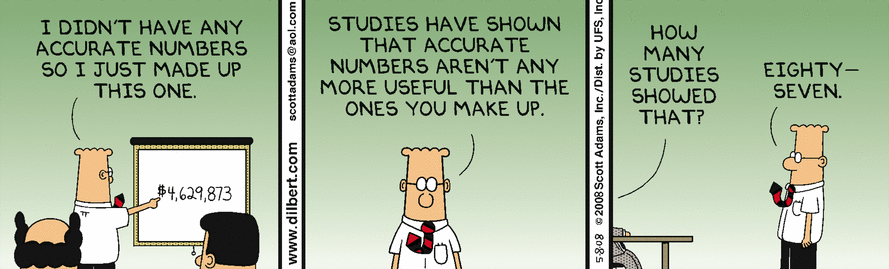
\includegraphics[scale=0.48]{dilbertStatistics.png}
\end{center}


\end{frame}




\begin{frame}{What People Talk about Statistics?}


\begin{shadequote}[r]{Bernie Siegel}
Stories change people while statistics give them something to argue about. 
\end{shadequote}

\begin{shadequote}[r]{Mark Twain}
Facts are stubborn, but statistics are more pliable.
\end{shadequote}

\begin{shadequote}[r]{George Bernard Shaw}
Statistics show that of those who contract the habit of eating, very few survive.
\end{shadequote}
\end{frame}


\begin{frame}{What People Talk about Statistics?}
\begin{shadequote}[r]{Edwards Deming}
In God we trust; all others must bring data.
\end{shadequote}

\begin{shadequote}[r]{Karl Pearson}
Statistics is the grammar of science.
\end{shadequote}

\begin{shadequote}[r]{Simeon Strunsky}
Statistics are the heart of democracy.
\end{shadequote}

\begin{shadequote}[r]{Thomas Carlyle}
A judicious man looks on statistics not to get knowledge, but to save himself from having ignorance foisted on him.
\end{shadequote}

\end{frame}


\begin{frame}{People Who Changed the World Using Statistics}

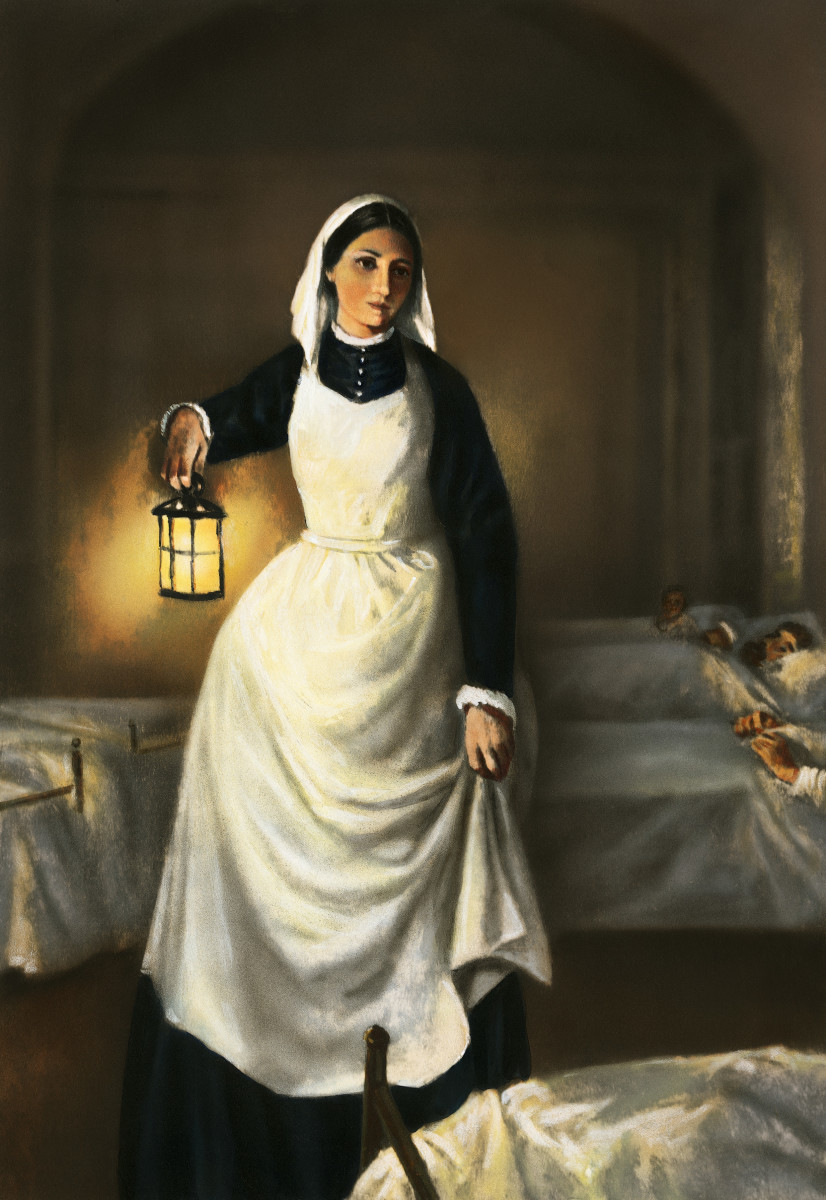
\includegraphics[height = 4.8 cm]{illustration-of-florence-nightingale-holding-lamp.jpg}
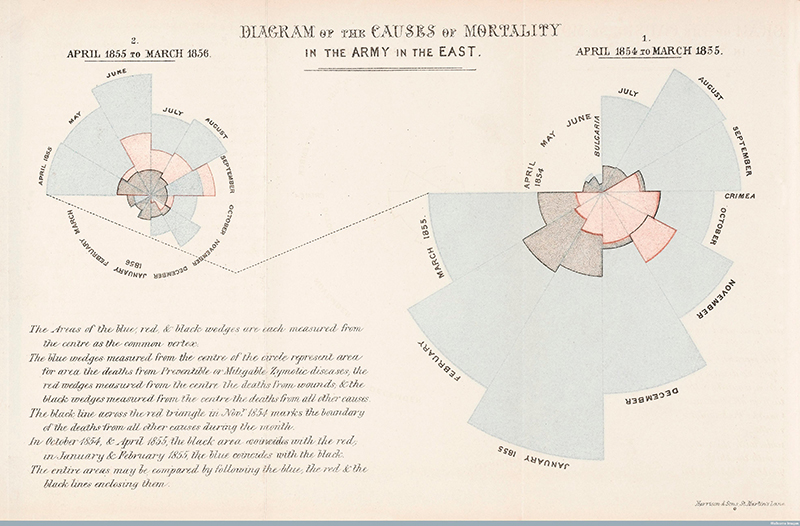
\includegraphics[height = 4.8 cm]{nightingaleChart.jpg}

By using applied statistical methods, Florence Nightingale (1820 - 1910) made a case for eliminating the practices that contributed to the unsafe and unhealthy environment.

\end{frame}


\begin{frame}{People Who Changed the World Using Statistics (cont.)}

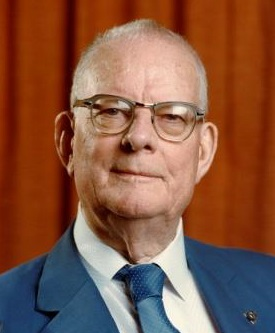
\includegraphics[height = 4.7 cm]{edwardDeming.jpg}

\includegraphics[height = 4.7 cm]{redBeads.png}

Dr. Edwards Deming found great inspiration in the work of Shewhart, the originator of the concepts of \textit{statistical control of processes} and the related technical tool of the control chart, as Deming began to move toward the application of statistical methods to industrial production and management.

\end{frame}


\begin{frame}{What is Statistics?}
About the word root:
\begin{itemize}
\item The term statistics is ultimately derived from the New Latin statisticum collegium ("council of state") and the Italian word statista ("statesman" or "politician"). - Wikipedia
\end{itemize}

\vspace{0.3 cm}

To define statistics: 
\begin{itemize}
\item Broadly, it refers to \textit{numerical facts} (e.g., mean, medians, percents, and index numbers) that help us understand a variety of business and economic situations.
\item Narrowly, it refers to \textit{the art and science} of                                  collecting, analyzing, presenting, and interpreting data. 
\end{itemize}

\end{frame}


\begin{frame}{Why is Statistics a Required Subject in Many Academic Discipline?}
\begin{itemize}
\item Statistics is the language of scientific exchanges
\item Statistics offers the guiding principles for scientific investigations
\item Statistics provides the mental frameworks for scientific experiments 
\item To sum, it is a language, methodology, and framework.
\item It is also a prerequisite to many other advanced courses in SCM, Marketing, Management, Finance, etc. 
\end{itemize}


\end{frame}


\subsection{What it can do for You?}


\begin{frame}{From Data to Knowledge}


\begin{multicols}{2}
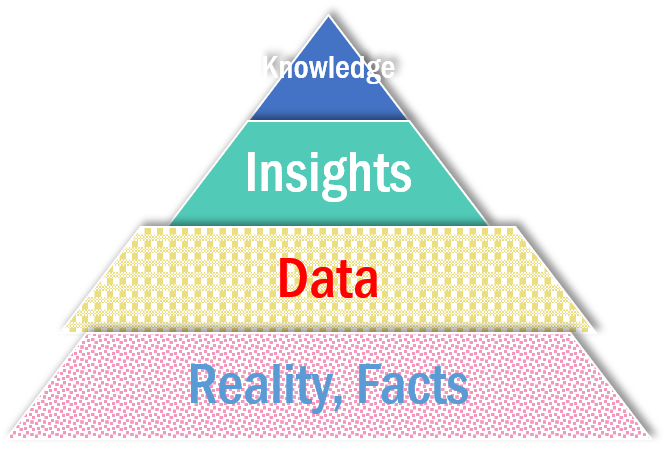
\includegraphics[scale=0.5]{images/dataToKnowledge.png}

\vspace{2cm}

\begin{itemize}
\item Data are the closest possible artifact to the reality.
\item The reality is messy and data are spurious.
\item Appropriate analysis is the key to extract insights from data.
\item Knowledge is nothing but validated insights.
\end{itemize}

\end{multicols}

\begin{shadequote}[r]{Arthur Conan Doyle}
It is a capital mistake to theorize before one has data. Insensibly one begins to twist facts to suit theories, instead of theories to suit facts.
\end{shadequote}

\end{frame}






\begin{frame}{Simpson's Paradox - UC Berkerley Gender Bias Case (1973)}


At a glance, in the school level, the gender differences in the admission is too large to be considered as a pure chance. 

\begin{table}
\centering
\resizebox{\linewidth}{!}}} & \multicolumn{1}{r|}{4,321} & \multicolumn{1}{r|}{35\%}  \\
\hline
\end{tabular}
}
\end{table}


\begin{scriptsize}
Source: 
Bickel, P. J., Hammel, E. A., \& O'Connell, J. W. (1975). Sex bias in graduate admissions: Data from Berkeley. \textit{Science}, 187(4175), 398-404.
\end{scriptsize}


\end{frame}



\begin{frame} {Simpson's Paradox - UC Berkerley Gender Bias Case (cont.)}

However, when examining the department level data, more departments appeared to be favoring women applicants. 

\begin{table}
\centering
\resizebox{\linewidth}{!}{%
\begin{tabular}{c|r|r|r|r} 
\hline
\multicolumn{1}{l|}{\multirow{2}{*}{Department}} & \multicolumn{2}{c|}{Men}                                          & \multicolumn{2}{c}{Women}                                         \\ 
\cline{2-5}
\multicolumn{1}{l|}{}                            & \multicolumn{1}{c|}{Applicants} & \multicolumn{1}{c|}{Admitted}   & \multicolumn{1}{c}{Applicants} & \multicolumn{1}{c}{Admitted}    \\ 
\hline
A                                                 & 825                             & 62\%                            & 108                             & \textbf{\textcolor{blue}{82\%}}  \\ 
\hline
B                                                 & 560                             & 63\%                            & 25                              & \textbf{\textcolor{blue}{68\%}}  \\ 
\hline
C                                                 & 325                             & \textbf{\textcolor{blue}{37\%}} & 593                             & 34\%                             \\ 
\hline
D                                                 & 417                             & 33\%                            & 375                             & 35\%                             \\ 
\hline
E                                                 & 191                             & \textbf{\textcolor{blue}{28\%}} & 393                             & 24\%                             \\ 
\hline
F                                                 & 373                             & 6\%                             & 341                             & \textbf{\textcolor{blue}{7\%}}   \\
\hline
\end{tabular}
}
\end{table}


\end{frame}



\begin{frame}{Careers Involving Statistics}



\begin{center}
\begin{tabular}{l|r|r}
\hline 
Job Title & Median Salary& Job Growth  \\ 
\hline 
Mathematician & \$101,900 & 26\% \\ 
\hline 
Market Research Analyst & \$63,120 & 20\% \\ 
\hline 
Meteorologist & \$94,110 & 8\% \\ 
\hline 
Statistician & \$87,780 & 31\% \\ 
\hline 
Operations Research Analyst & \$83,390 & 26\% \\ 
\hline 
Financial Analyst & \$85,660 & 6\% \\ 
\hline 
\end{tabular} 
\end{center}

\begin{scriptsize}
* Salary data year 2018; Job growth projection during 2018-2028\linebreak
* Source: U.S. Bureau of Labor Statistics \linebreak
* Originally from Study.com
\end{scriptsize}

\end{frame}


\begin{frame}{It's Now or Never!}

\begin{center}

\includegraphics[scale=0.30]{images/nowOrNever.jpg}
\end{center}

\end{frame}



\section{I. Review of Fundamentals}



\subsection{Section 1. Data Types}
\begin{frame}{Various Ways of Classifying Data}

Based on the Scales of Measurement
\begin{itemize}
\item Nominal, Ordinal, Interval, and Ratio
\end{itemize}

Based on the Nature of the Data
\begin{itemize}
\item Categorical (or qualitative) and Quantitative Data
\end{itemize}

Based on the Continuous Scale
\begin{itemize}
\item Binary (or dichotomous), Discrete, and Continuous Data
\end{itemize}

Based on the Temporality 
\begin{itemize}
\item Cross-sectional and Time Series Data
\end{itemize}

\end{frame}


\begin{frame}{The Scales of Measurement}

% Please add the following required packages to your document preamble:
% \usepackage{multirow}
% \usepackage{graphicx}
\begin{table}[]
\resizebox{\textwidth}{!}{%
\begin{tabular}{l|l|l}
\hline
\textbf{Scale Type}             & \textbf{Defined}                                      & \textbf{Examples}                \\ \hline
\multirow{2}{*}{Nominal}        & Data are labels or names used                         & Names: "John Doe", "Jane Doe"    \\
                                & to identify an attribute of the element.              & Labels: "NY", "OH", "MI"         \\ \hline
\multirow{2}{*}{Ordinal}  & The data have the properties of nominal data AND      & Rating: "Good", "Neutral", "Bad" \\
                                & the order or rank of the data is meaningful.          & Rank: "First", "Second", "Third" \\ \hline
\multirow{3}{*}{Interval} & The data have the properties of ordinal data AND      & Temperature: 0, 3.4, 5.6, 3, 4   \\
                                & the interval between observations is expressed        &                                  \\
                                & in terms of a fixed unit of measure.                  &                                  \\ \hline
\multirow{2}{*}{Ratio}    & The data have all the properties of interval data  & Height: 5 ft.; Weight: 3 lbs.       \\
                                & AND the ratio of two values is meaningful.                & Debt amount: \$345,000           \\ \hline
\end{tabular}%
}
\end{table}

\end{frame}

\begin{frame}{Comparing Different Scales of Measurement}


\begin{table}[]
\resizebox{\textwidth}{!}{%
\begin{tabular}{l|c|c|c|c}
\hline
\textbf{Characteristics}                                       & \multicolumn{1}{l|}{\textbf{Nominal}} & \multicolumn{1}{l|}{\textbf{Ordinal}} & \multicolumn{1}{l|}{\textbf{Interval}} & \multicolumn{1}{l}{\textbf{Ratio}} \\ \hline
The order of values is meaningful                   &                              & Y                            & Y                             & Y                          \\ \hline
"Count" matters                                & Y                            & Y                            & Y                             & Y                          \\ \hline
An arithmetic mean has meaning                &                              & Y                            & Y                             & Y                          \\ \hline
Can quantify the difference &                              &                              & Y                             & Y                          \\ \hline
Can add or subtract values                     &                              &                              & Y                             & Y                          \\ \hline
Can multiply and divide values                 &                              &                              &                               & Y                          \\ \hline
"Zero" has meaning                             &                              &                              &                               & Y                          \\ \hline
\end{tabular}%
}
\end{table}
\end{frame}


\begin{frame}{Example of the Data Type}

\begin{center}
\textit{Q: Can you tell what scale of measurement each column uses? 
}
\end{center}
\begin{center}
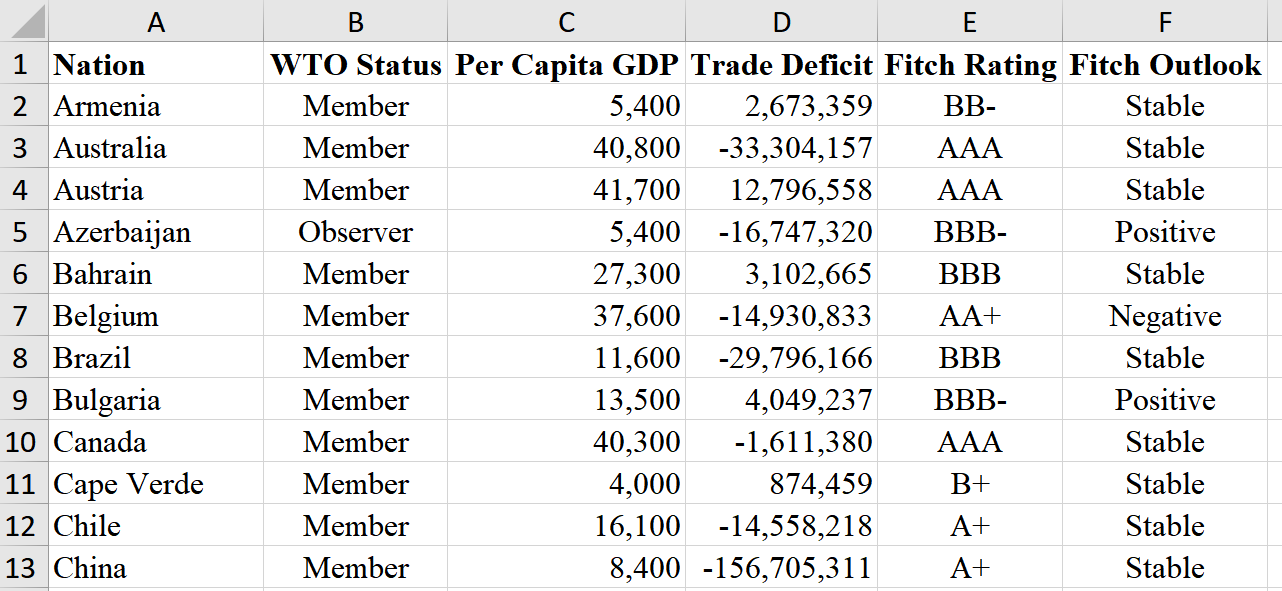
\includegraphics[scale=0.55]{images/scaleTypeDataExample.png}
\end{center}
\begin{scriptsize}
Data Source: Textbook Data, Only the first 12 observations are shown.
\end{scriptsize}
\end{frame}





\begin{frame}{Data on the Continuous Scale}

Data can also classified based on the accuracy of the measurement.

\vspace{10pt}
\begin{itemize}
\item Binary Scale
\begin{itemize}
\item Only considers two cases or two levels: "Yes" or "No", "Success" or "Failure", "Before" or "After".
\item Convenient in calculating the proportion. 
\end{itemize}
\item Discrete Scale
\begin{itemize}
\item Similar with the ordinal scale, the discrete data can be measured using integers.
\item Convenient when outcomes have limited results.
\end{itemize}

\item Continuous Scale
\begin{itemize}
\item Can take any real number (positive, negative, integer, \& fraction).
\item Allows many advanced statistical analysis.
\end{itemize}
\end{itemize}

\end{frame}


\begin{frame}{Cross-Sectional Data}

The cross-sectional and time-series distinction is more about the entire dataset, rather about a specific column. 

\begin{center}
A cross-sectional dataset provides a snapshot on a specific time point. 
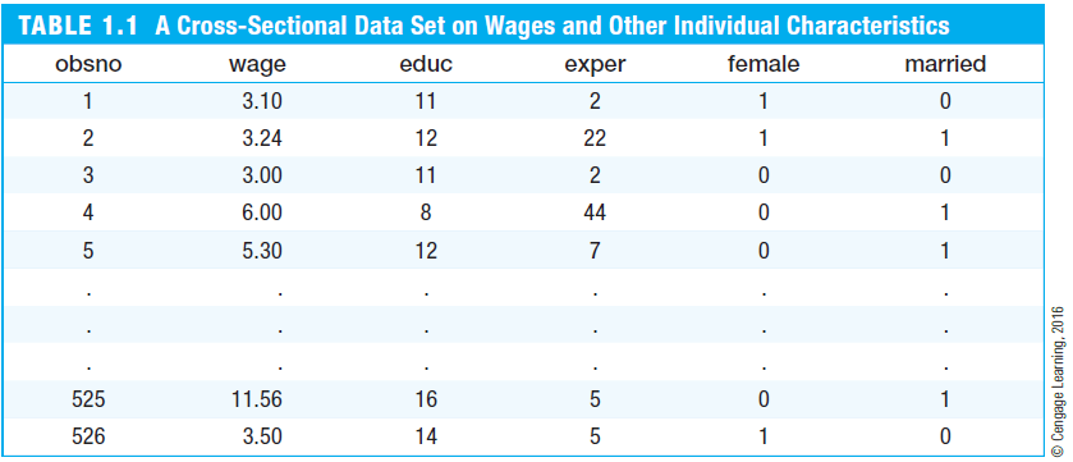
\includegraphics[scale=0.4]{images/crossSectional.png}
\end{center}
\begin{scriptsize}
Source: Woodridge (6th Ed.)
\end{scriptsize}
\end{frame}


\begin{frame}{Time-series Data}

\begin{center}
A time-series data observes the same entity overtime. 
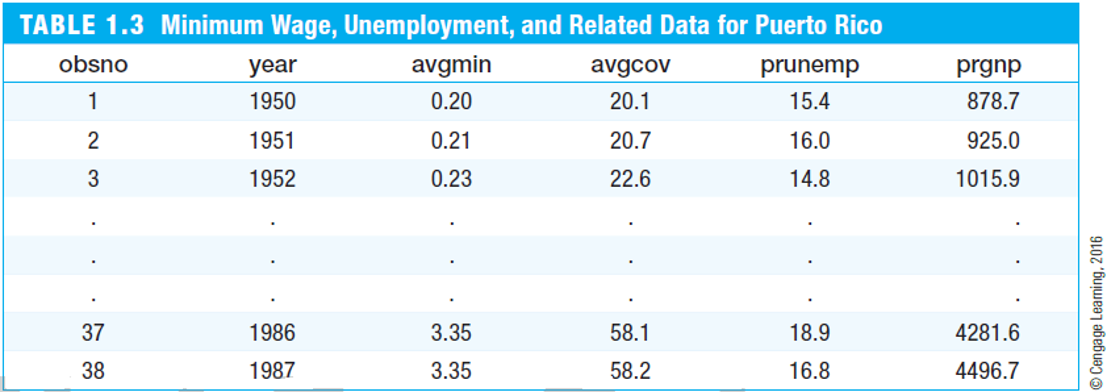
\includegraphics[scale=0.36]{images/timeSeries.png}
\end{center}
\begin{scriptsize}
Source: Woodridge (6th Ed.)
\end{scriptsize}
\end{frame}



\begin{frame}{Check your understanding 1/3}

Q: Some hotels ask their guests to rate the hotel's services as excellent, very good, good, and poor. This is an example of the

\vspace{5 pt}

a.	ordinal scale of measurement \linebreak
b.	ratio scale of measurement \linebreak
c.	nominal scale of measurement \linebreak
d.	interval scale of measurement


\end{frame}



\begin{frame}{Check your understanding 2/3}

Q: The scale of measurement that has an inherent zero value defined is the

\vspace{5 pt}

a.	ratio scale \linebreak
b.	nominal scale \linebreak
c.	ordinal scale \linebreak
d.	interval scale

\end{frame}

\begin{frame}{Check your understanding 3/3}

Q: Data collected over several time periods are

\vspace{5 pt}

a.	time series data \linebreak
b.	time controlled data \linebreak
c.	cross-sectional data \linebreak
d.	time cross-sectional data

\end{frame}



\subsection{Section 2. Common Math Notations}

\begin{frame}{Common Math Notations: Series, Index, and Sum}
Use \textbf{index letter} $i$ or $j$ to enumerate multiple observations from the same series (for example, a column)
$$ x_i = \lbrace x_1, x_2, x_3, ... x_I\rbrace $$
In combination with the \textbf{sum notation} $\sum$, the indexing makes the calculation of the \textit{series sum} very convenient. (A column total)
$$ \sum_{i=1}^{I}x_i = x_1 + x_2 + x_3 + ... + x_{I}$$

\begin{small}
\textit{(The summation in plain English: Add the first element from $x$ to $I$th element.)} 
\end{small}




\end{frame}


\begin{frame}{Common Math Notations (cont.)}

One example of the series sum where each element of the series is reduced by a constant value $k$
$$ \sum_{i=1}^{I}(x_i - k) = (x_1 - k) + (x_2 - k) + (x_3 - k) + ... + (x_I - k)$$


\end{frame}



\begin{frame}{Check your Understanding 1/2}
Consider the following example ($k=5$): 
\begin{center}
\begin{tabular}{c|c|c|c}
\hline 
\rule[-1ex]{0pt}{2.5ex} $i$ & $x_i$ & $x_i - k$ & $x_i \times k$ \\ 
\hline 
\hline 
\rule[-1ex]{0pt}{2.5ex} 1 & 32 & 27 & 160 \\ 
\hline 
\rule[-1ex]{0pt}{2.5ex} 2 & 41 & 36 & 205 \\ 
\hline 
\rule[-1ex]{0pt}{2.5ex} 3 & 57 & 52 & 285 \\ 
\hline 
\hline 
\rule[-1ex]{0pt}{2.5ex} Total & 130 & 115 & 650 \\ 
\hline 
\end{tabular} 
\end{center}

\begin{itemize}
\item Can you use the summation symbol and index letter to express the summation of each column? 

\end{itemize}

\end{frame}


\begin{frame}{Check your Understanding 2/2}
What's the difference: $\sum_{i=1}^{N}(x_i - k) $ vs. $\sum_{i=1}^{N}x_i - k $?

\end{frame}



\begin{frame}{Naming Conventions: True vs. Observed Values}
To simplify the expression, we stick to the following naming conventions. There are largely two groups:
\begin{itemize}
\item One group is the \textit{true values}. We don't always get to observe these values but we wish to know. 
\item The other group is the \textit{observed values}. We can always observe these values through samples. 
\end{itemize}

\begin{center}


\begin{small}
\begin{tabular}{l|c|c}
\hline
                   & True Value   & Observed Value   \\
\hline
\hline
Mean               & $\mu$        &  $\bar{x}$       \\
\hline
Standard Deviation & $\sigma$      &  $s$              \\
\hline
Variance           & $\sigma^2$   & $s^2$        \\
\hline
Proportion         & $p$          & $\bar{p}$ \\
\hline
Correlation        & $\rho$       & $r$     \\
\hline
Size of the Observation        & $N$       & $n$     \\
\hline
\end{tabular}
\end{small}

\end{center}

\end{frame}


\begin{frame}{Check Your Understanding}
Can you explain the following expressions verbally? 
$$ \sigma = \sqrt{\frac{\sum_{i=1}^I(x_i - \mu)^2}{N}}$$


$$ s = \sqrt{\frac{\sum_{i=1}^I(x_i - \bar{x})^2}{n-1}}$$

Hint: If a calculation involves a series such as $x_i$, it is convenient to use a tabular approach to solve the problem. 

\end{frame}



\section{II. Descriptive Statistics}




\begin{frame}{Introduction to Descriptive Statistics}

Descriptive statistics is a set of techniques that are being used to summarize a given data.


% Please add the following required packages to your document preamble:
% \usepackage{graphicx}
\begin{table}[]
\caption{Frequently Used Descriptive Statistics}
\label{tab:my-table}
\resizebox{\textwidth}{!}{%
\begin{tabular}{l|l|l|l}
\hline
                    & \textbf{Graphical}         & \textbf{Tabular}         & \textbf{Numerical}                                                                      \\ \hline
Single Categorical  & Bar Chart         & Frequency Table &                                                                                \\ \hline
Single Quantitative & Histogram         & Frequency Table & Mean, S.d.                                                                     \\ \hline
Two Categorical     & Stacked Bar Chart & Crosstabulation &                                                                                \\ \hline
Two Quantitative    & Scatter Plot      & Crosstabulation & \begin{tabular}[c]{@{}l@{}}Covariance, \\ Correlation Coefficient\end{tabular} \\ \hline
\end{tabular}%
}
\end{table}


\begin{center}
\textit{There are many more and you can get really creative in terms of using visual elements to communicate.
}\end{center}

\end{frame}



\begin{frame}{Some Fancy Visualization Examples (1/2)}

\begin{center}
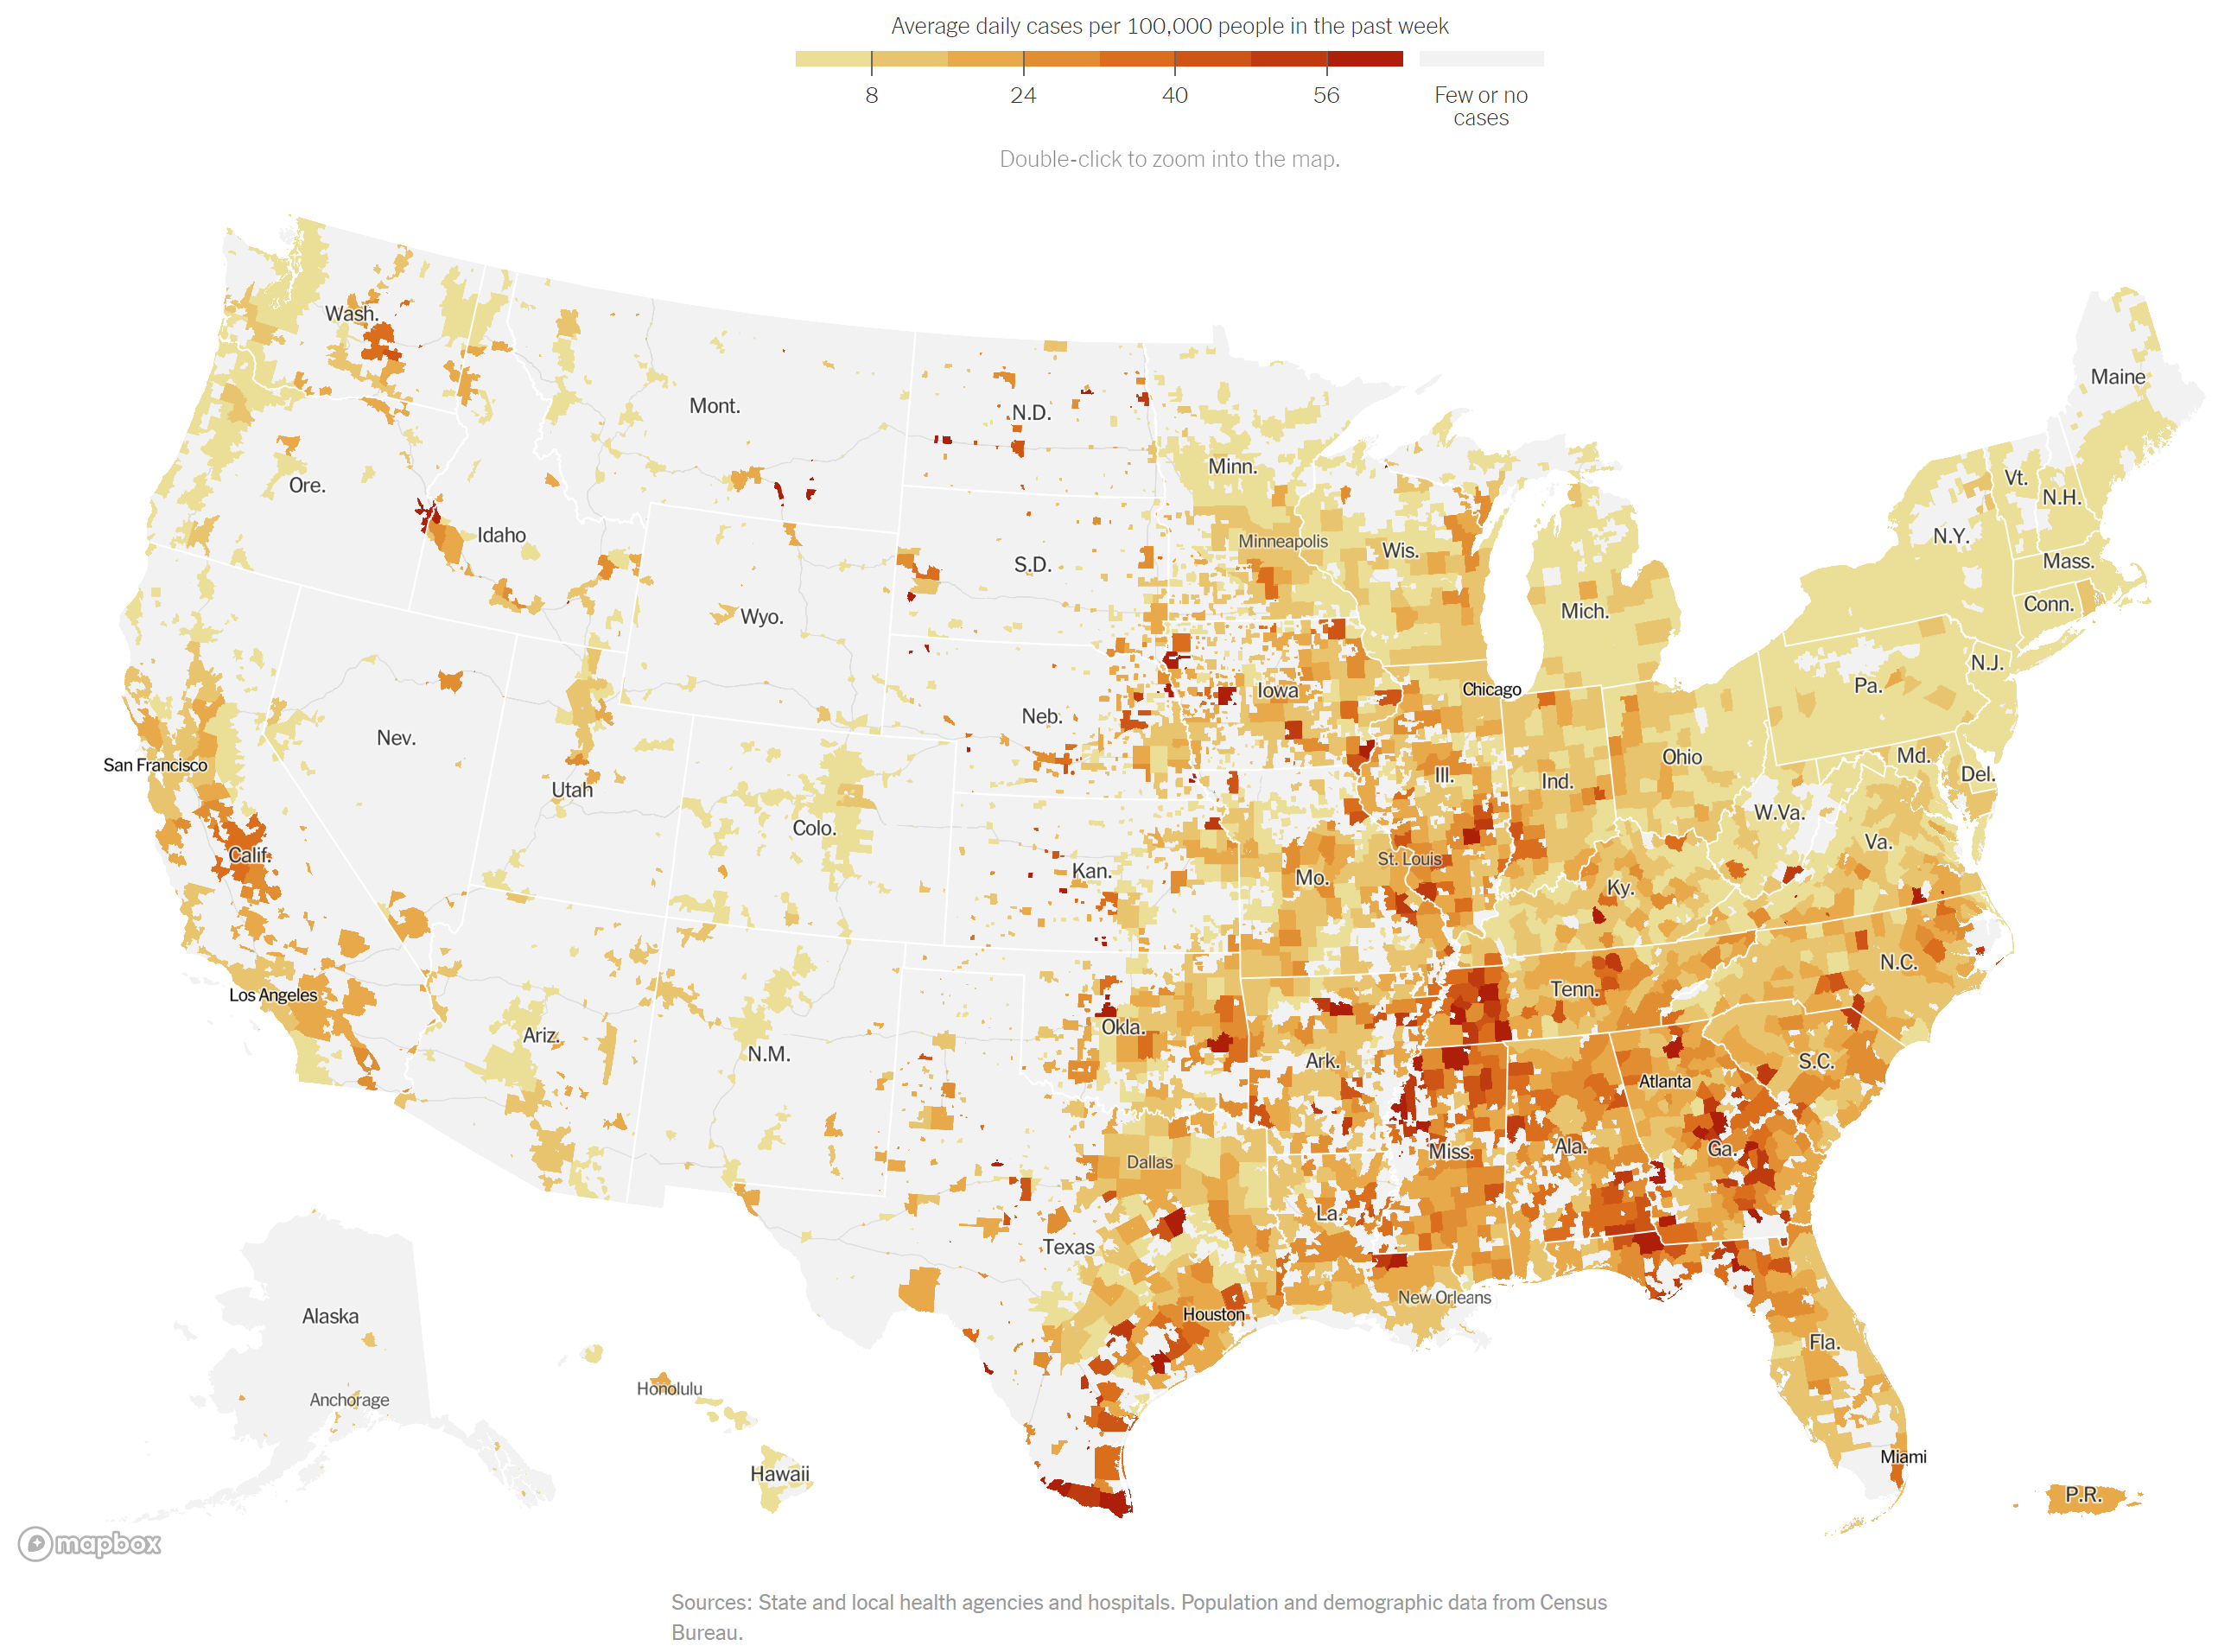
\includegraphics[scale=0.25]{images/covidVisualization1.png}

\end{center}

\end{frame}



\begin{frame}{Some Fancy Visualization Examples (2/2)}

\begin{center}
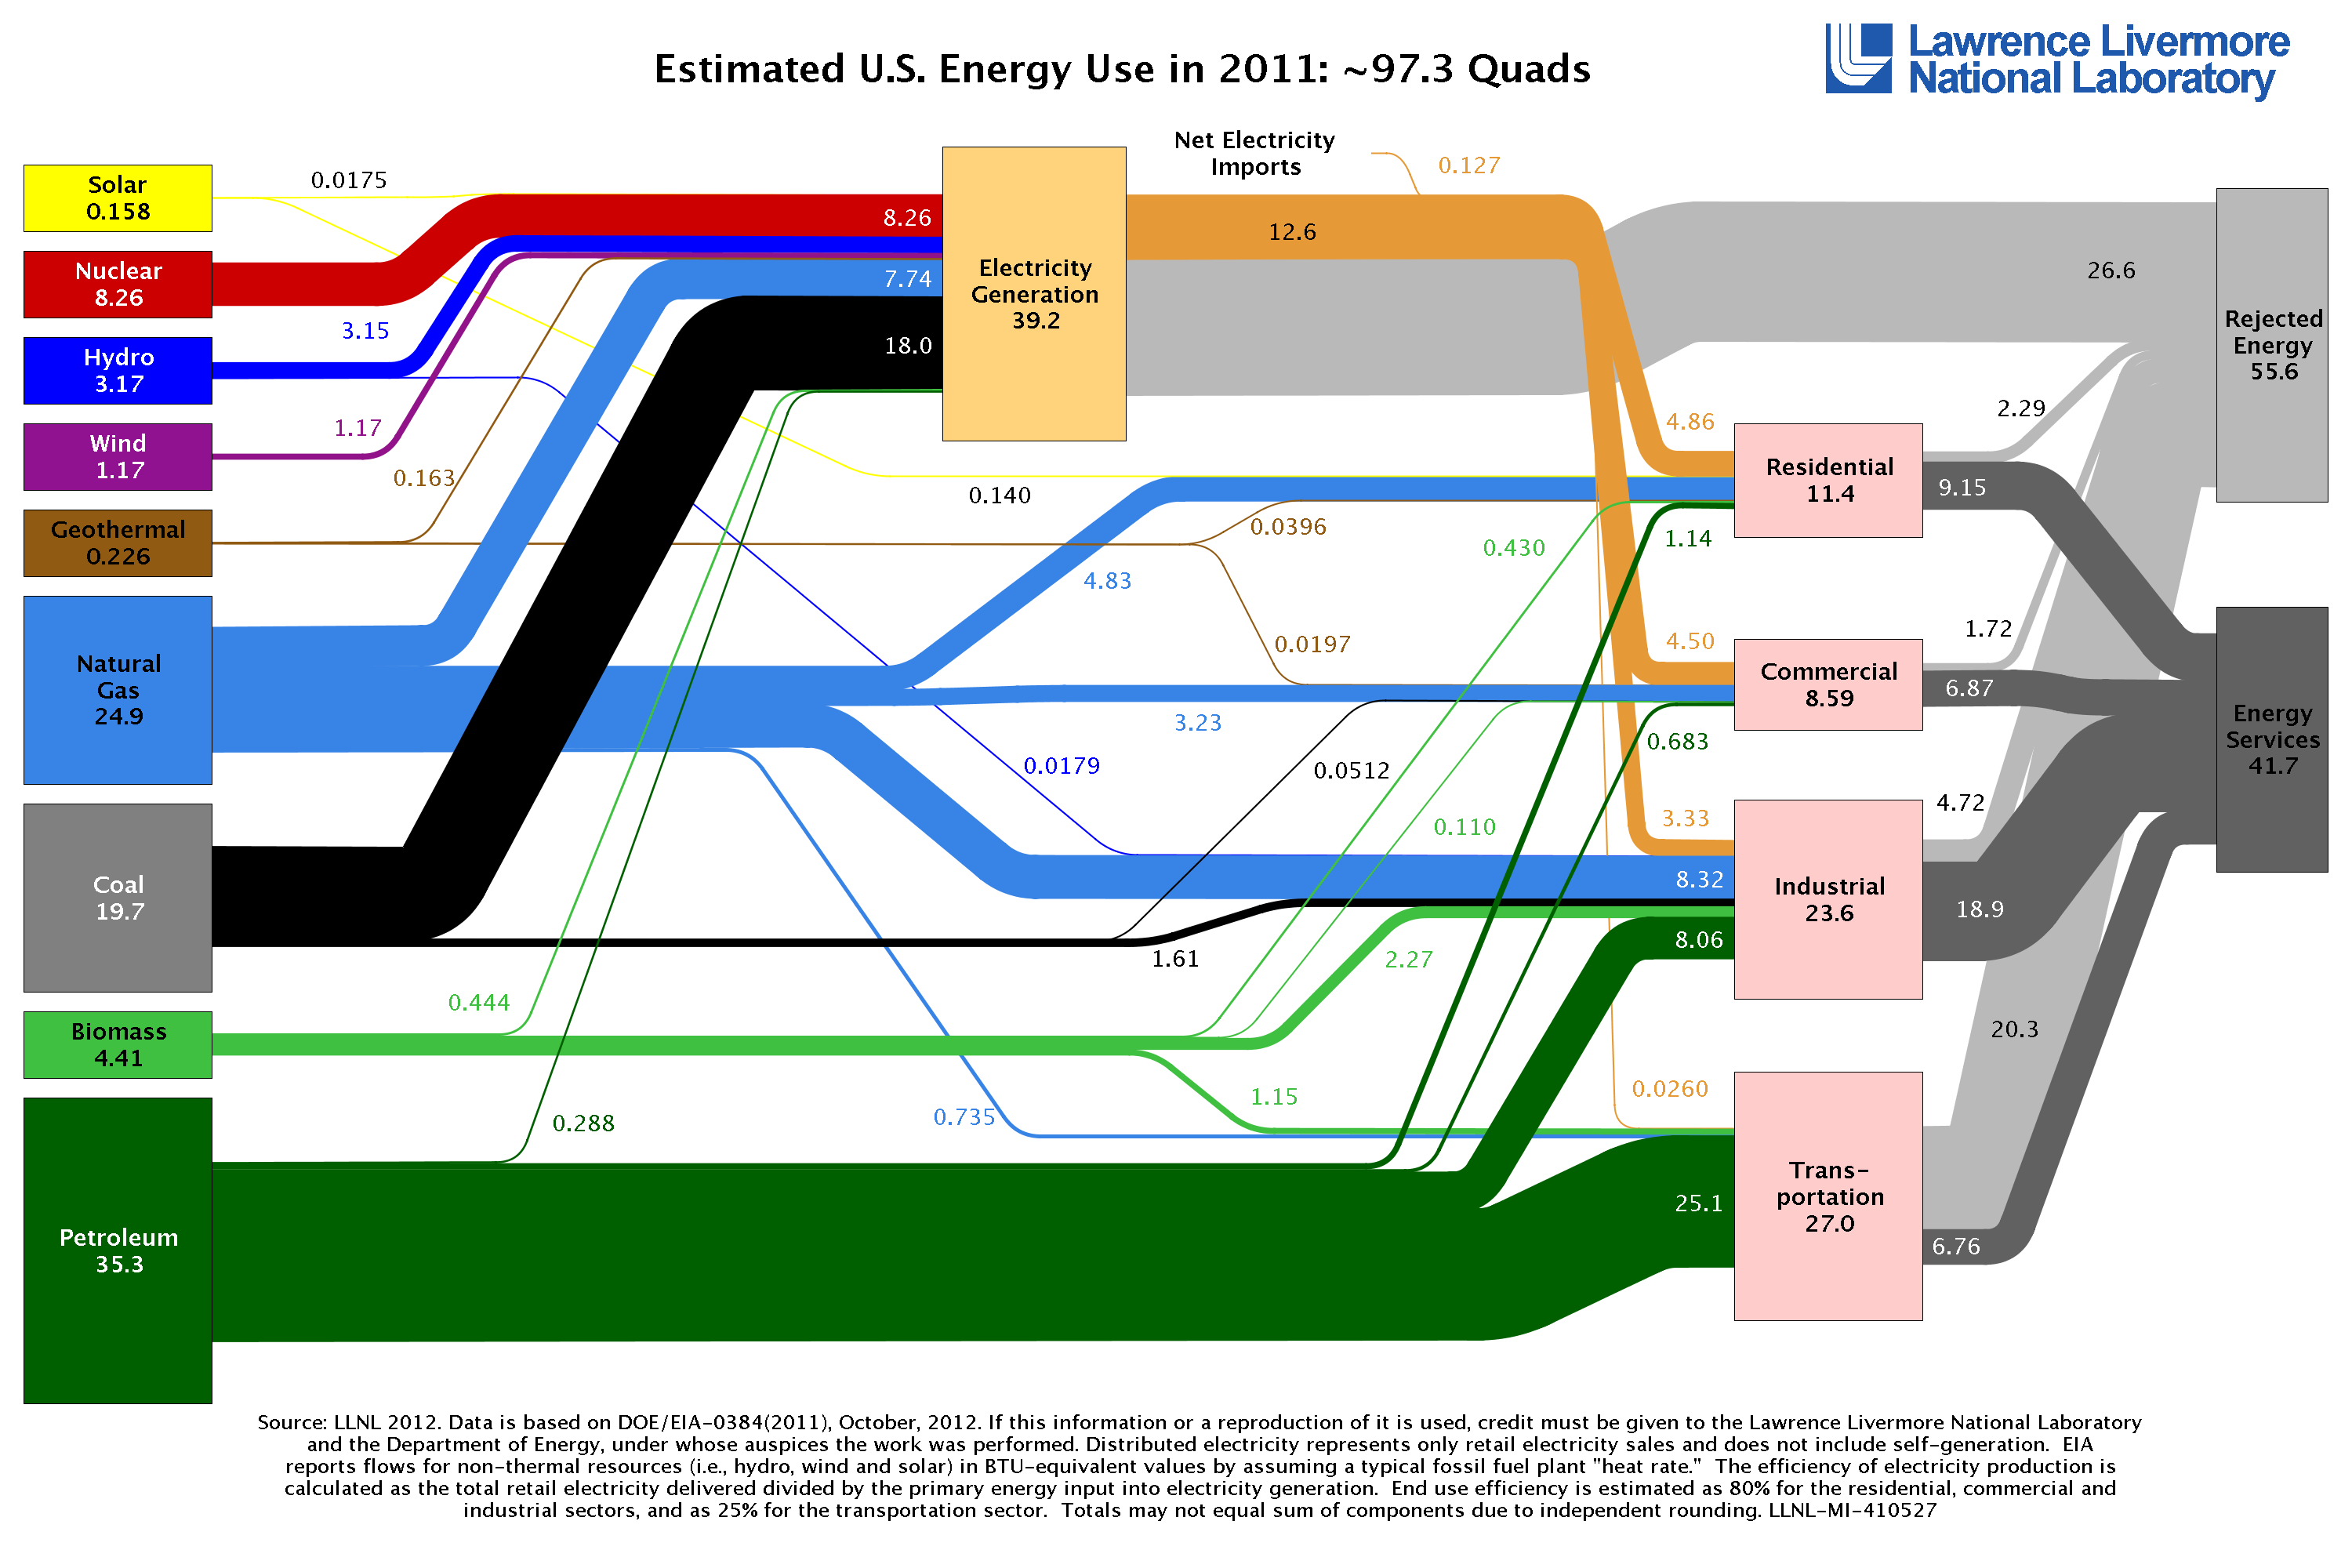
\includegraphics[scale=0.1]{images/ch2visualization2.png}

\end{center}

\end{frame}




\subsection{Section 1. Tabular and Graphical Summary}

\begin{frame}{Exhibition of the Data - \textit{Ch2. PelicanStores.xlsx}}

\begin{center}
(Note: to save space, only showing the first and the last five observations. Originally $n = 100$)
\vspace{0.5cm}

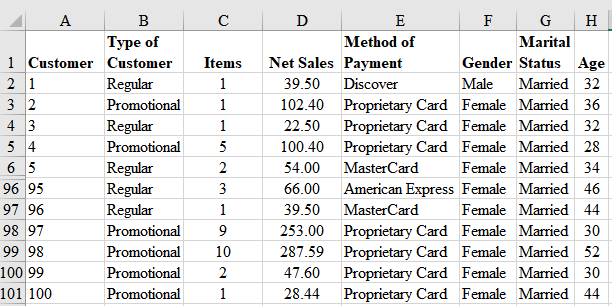
\includegraphics[scale=0.7]{images/ch2PelicanDataSnippet.png}
\end{center}


\end{frame}

\subsubsection{Frequency Analysis, Pie Chart, and Bar Chart}
\begin{frame}{Summarizing One Categorical Variable - Frequency Analysis}

\begin{center}
\textit{Method of Payment} Variable (or Column)
\vspace{0.5 cm}

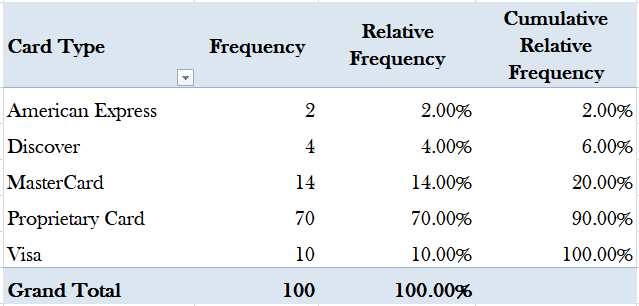
\includegraphics[scale=0.6]{images/frequencyTable.png}

\vspace{0.5cm}
\textit{This information will become the basis for many visualization.
}
\end{center}

\end{frame}


\begin{frame}{Summarizing One Categorical Variable - Pie Chart}

\begin{center}
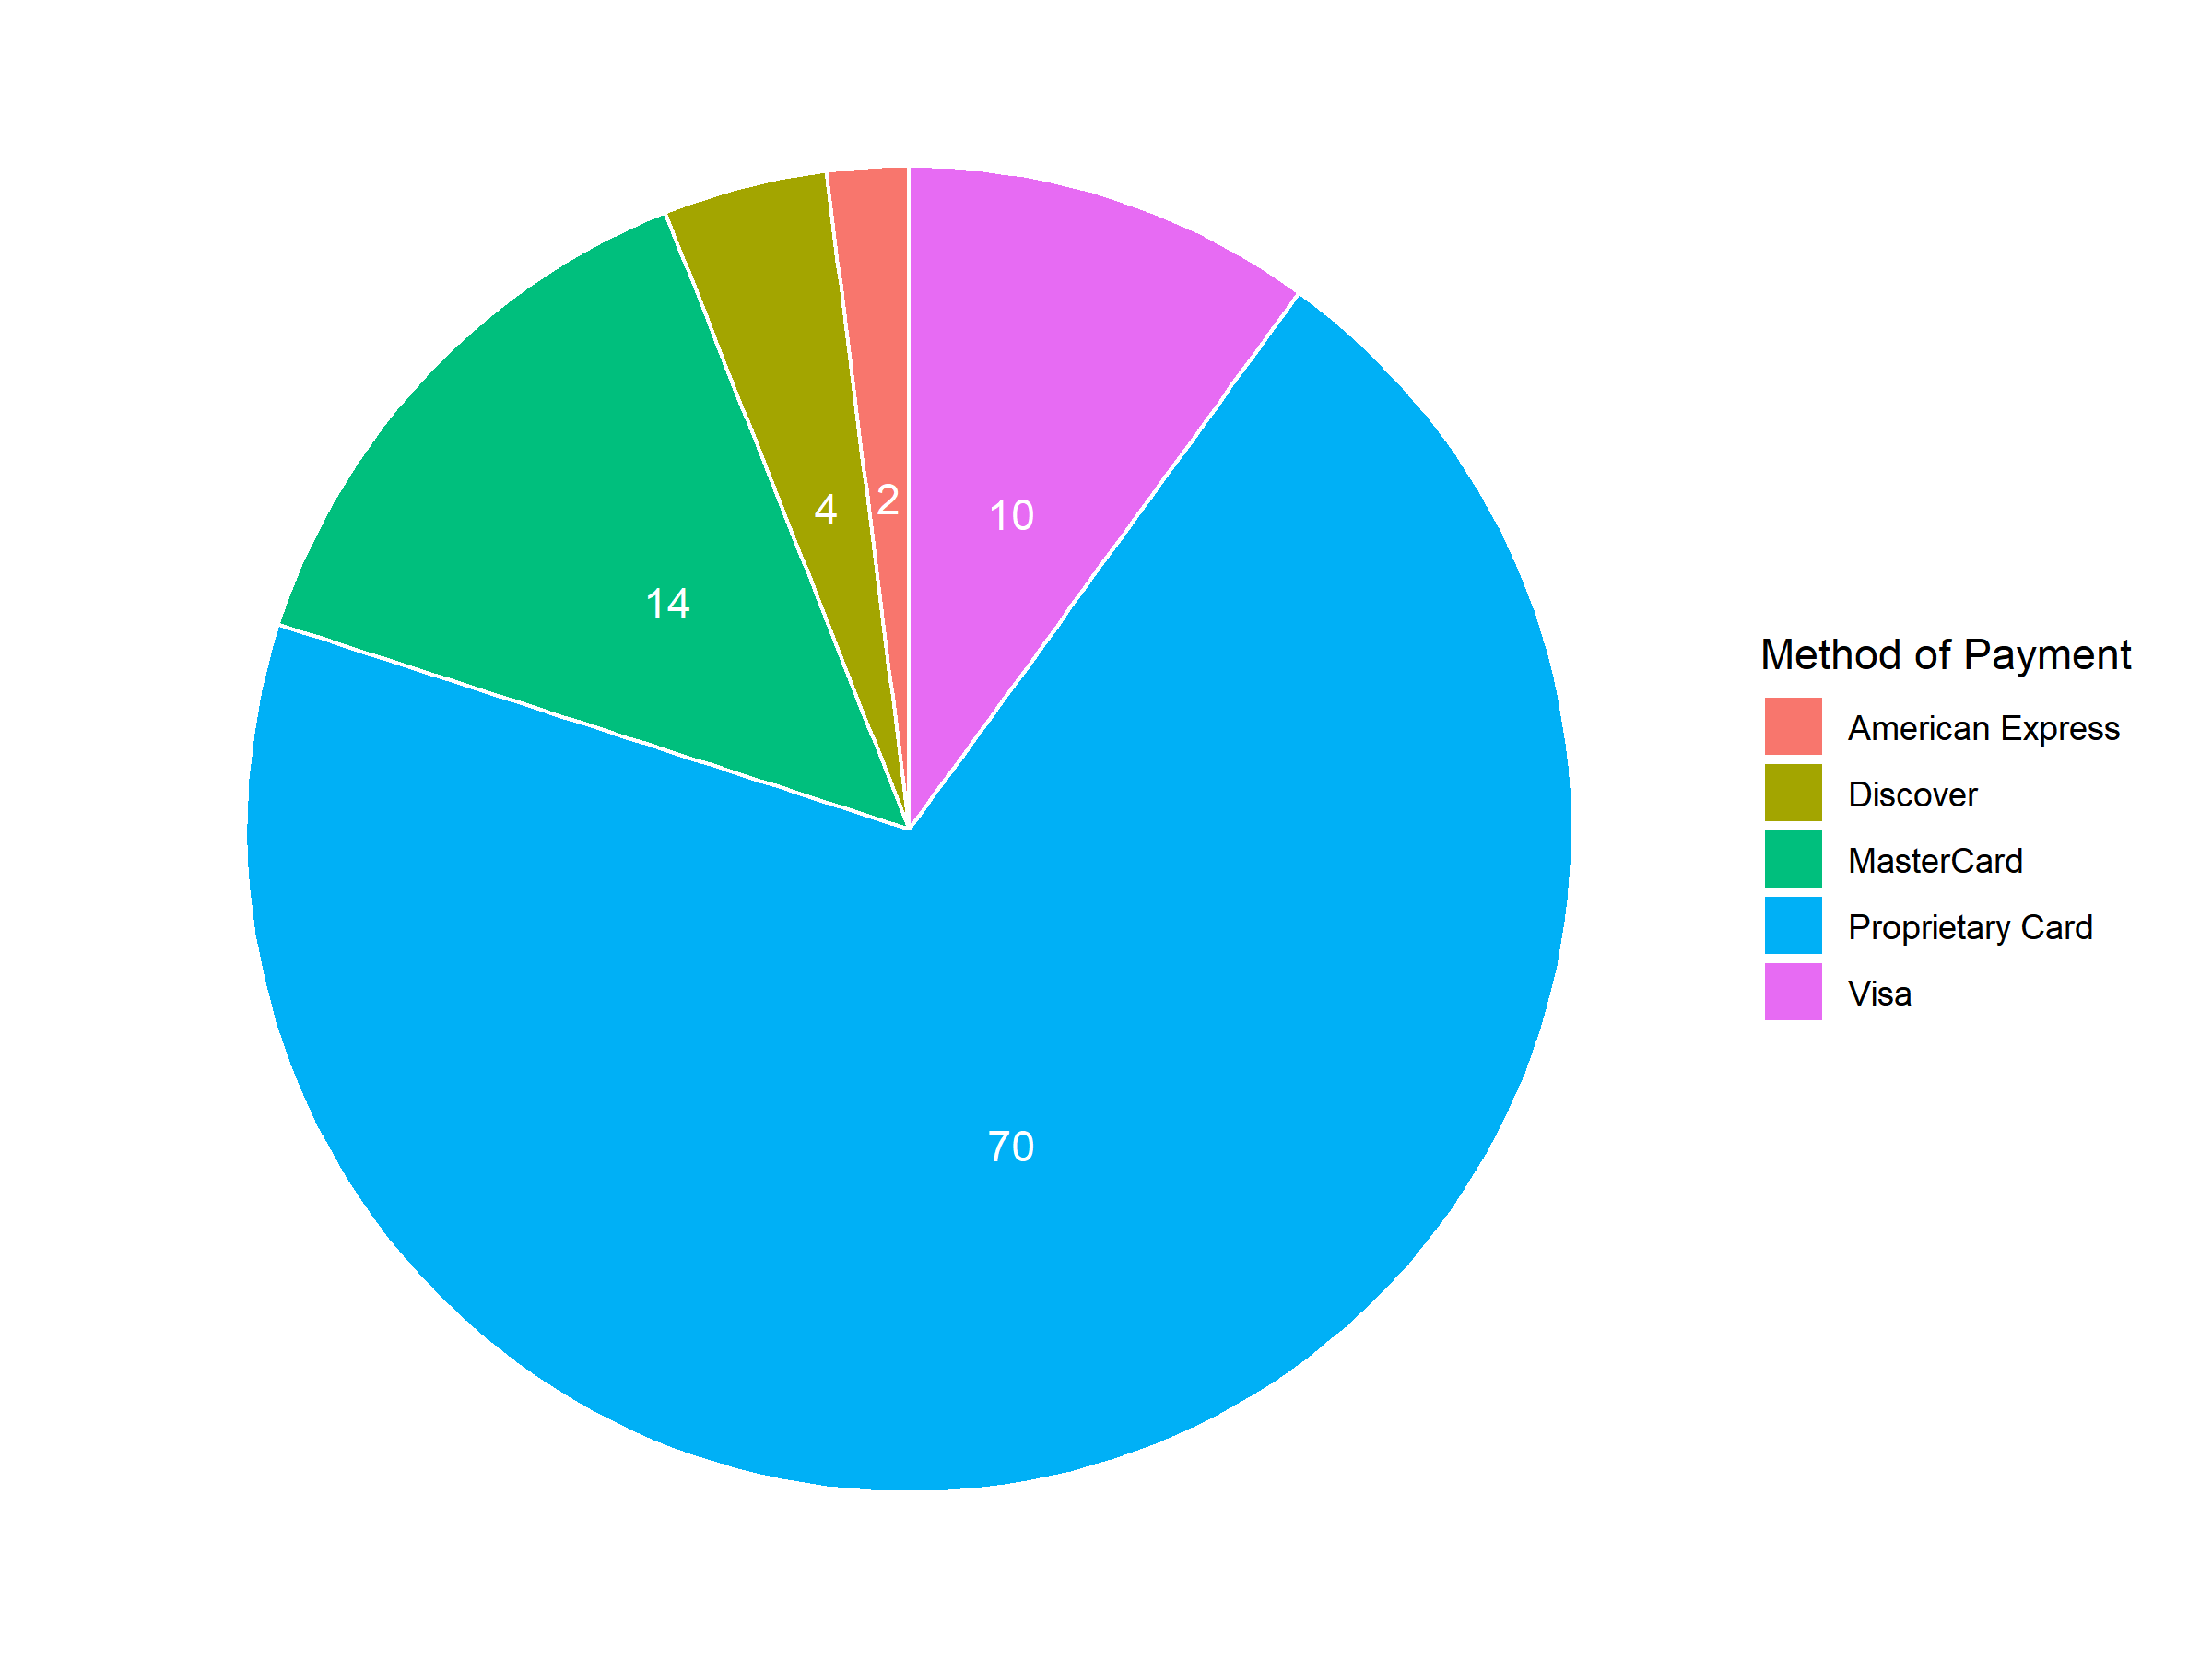
\includegraphics[scale=.45]{images/ch2PieChart.png}

\textit{The size of the angle for each "pie slice" represents the relative frequency of the category. 
}
\end{center}
\end{frame}


\begin{frame}{Summarizing One Categorical Variable - Bar Chart}

\begin{center}
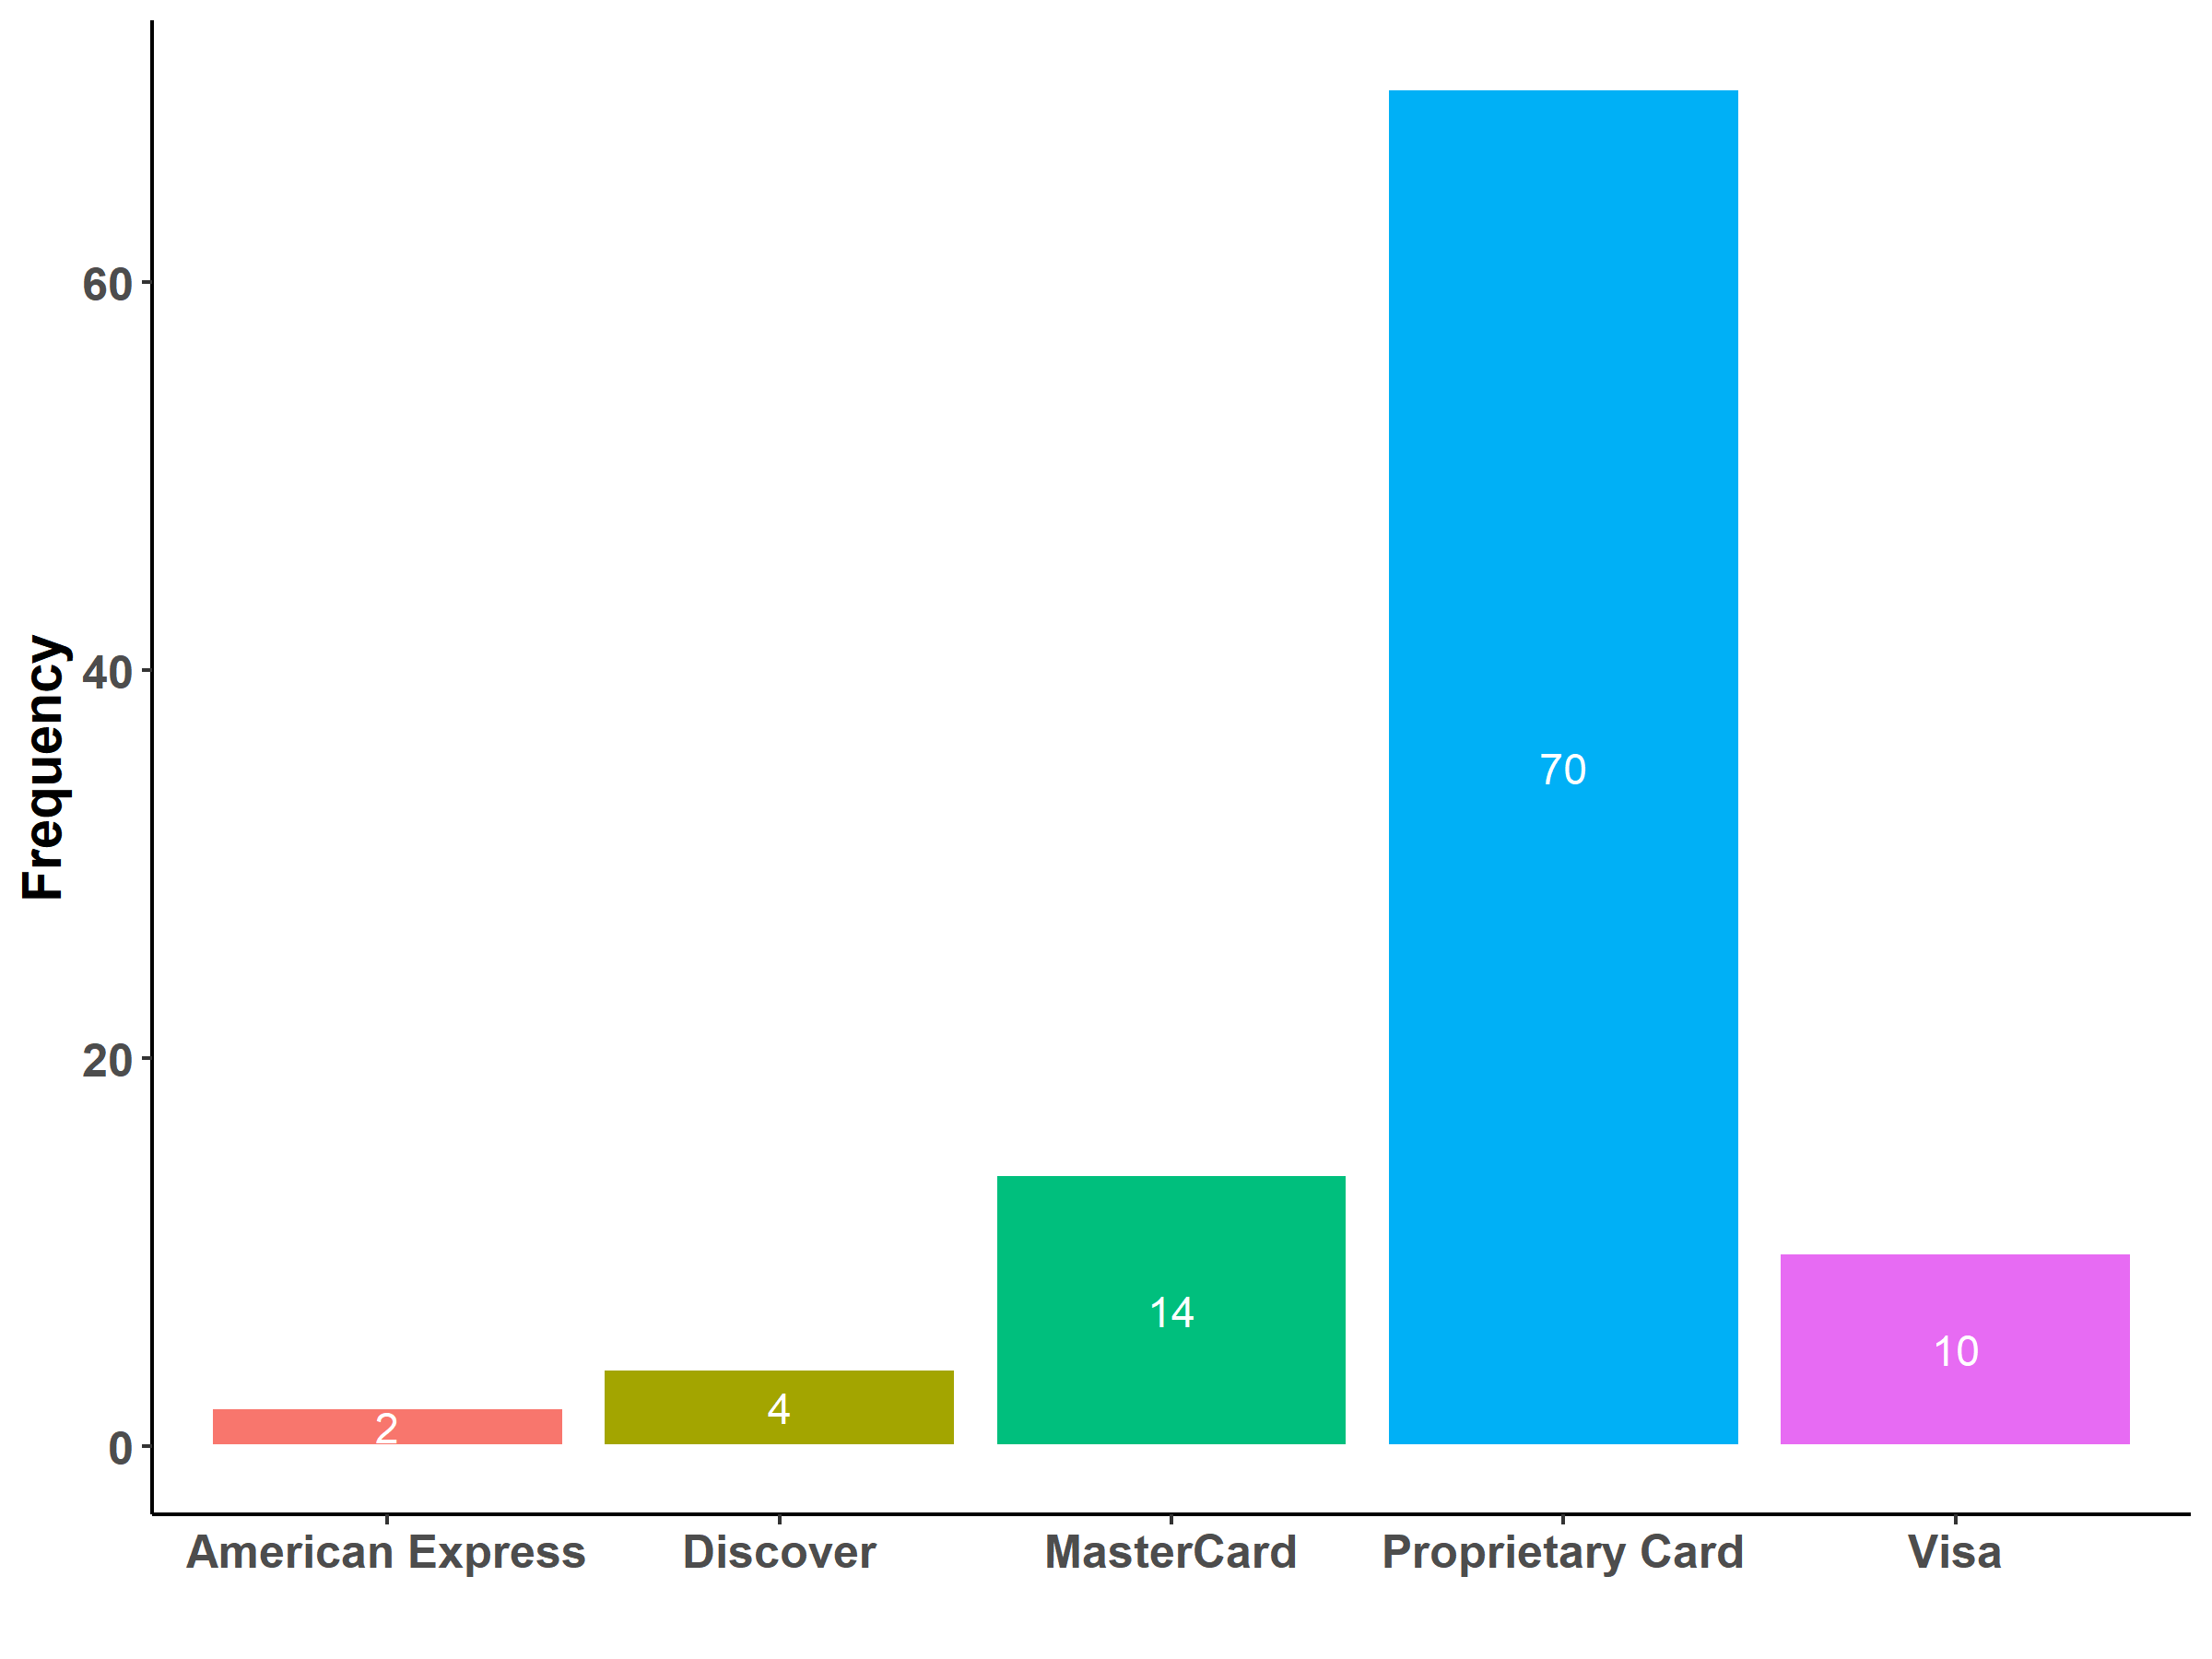
\includegraphics[scale=.45]{images/ch2BarChart.png}

\textit{The height of each bar represents the frequency of the category. 
}
\end{center}


\end{frame}


\begin{frame}{Summarizing One Continuous Variable - Frequency Analysis}

\begin{center}
\textit{Net Sales} Variable
\vspace{0.25 cm}

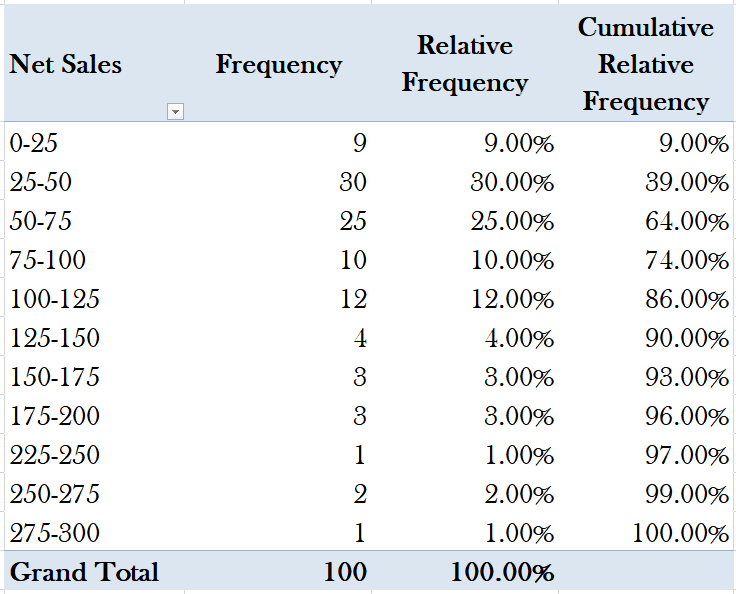
\includegraphics[scale=0.4]{images/ch2ContinuousFrequencyTable.png}
\end{center}

\end{frame}

\subsubsection{Histogram}
\begin{frame}{Summarizing One Continuous Variable - Histogram (1/5)}

\begin{center}

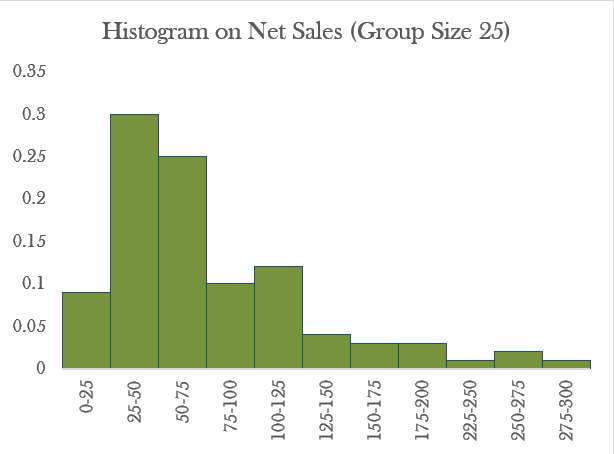
\includegraphics[scale=0.5]{images/ch2Histogram.png}
\end{center}

\begin{center}
\textit{The height of each bar represents the frequency of the group.
}
\end{center}

\end{frame}


\begin{frame}{Summarizing One Continuous Variable - Histogram (2/5)}

\begin{center}

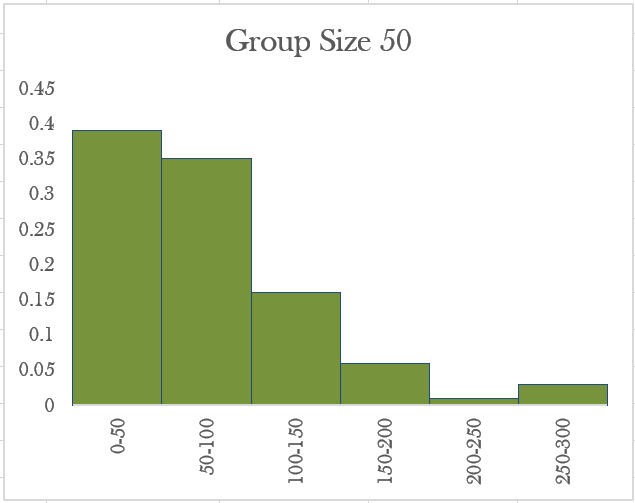
\includegraphics[scale=0.31]{images/ch2Histogram1.png}
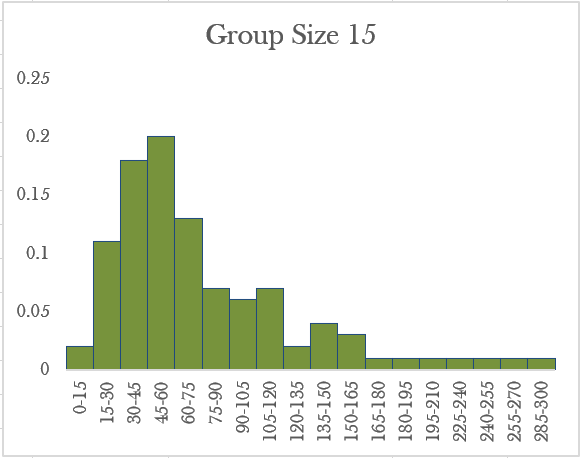
\includegraphics[scale=0.34]{images/ch2Histogram2.png}
\end{center}


\begin{scriptsize}
\begin{itemize}
\item Depending on the group size of choice, you may ended up obtain very different looking histogram on the same variable.
\item The width (or size) of a group is determined by the number of groups you are planning to use. 

\end{itemize}

$$ \textsf{Group Width} = \frac{Max(x_i)-Min(x_i)}{\textsf{Group Number}}$$

\end{scriptsize}



\end{frame}

\begin{frame}{Summarizing One Continuous Variable - Histogram (3/5)}

\begin{center}

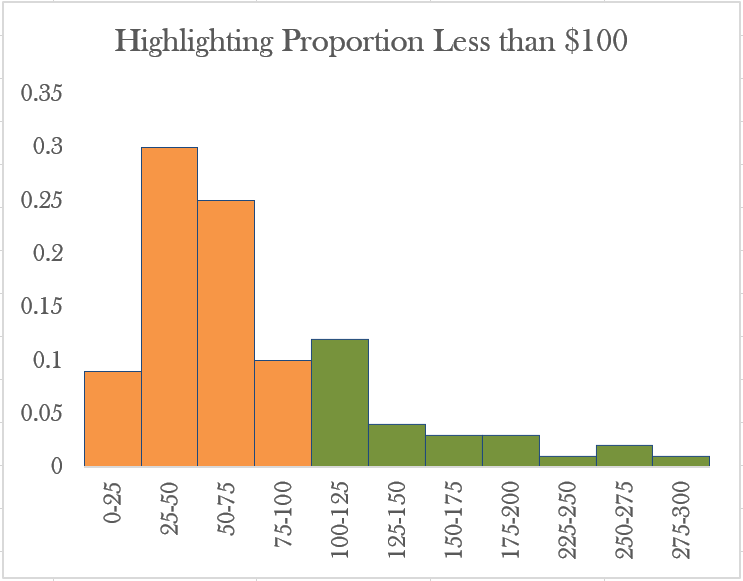
\includegraphics[scale=0.27]{images/ch2Histogram3.png}
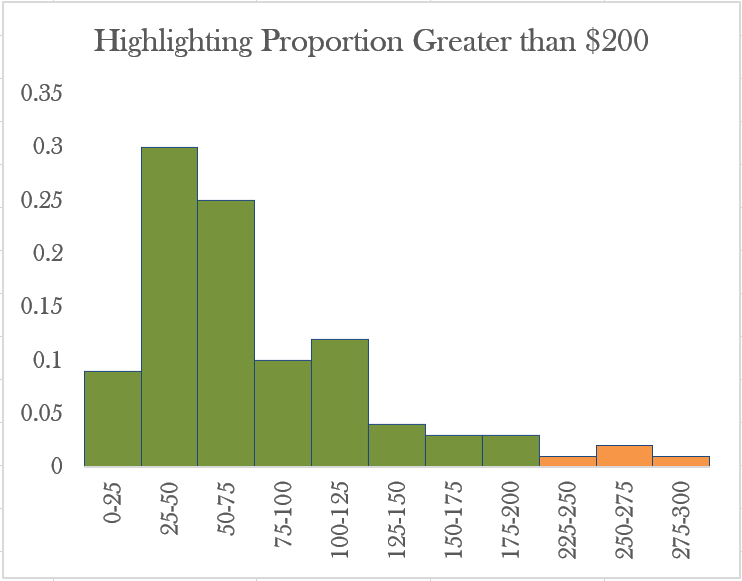
\includegraphics[scale=0.27]{images/ch2Histogram4.png}
\end{center}

\begin{center}
\textit{Because all bars are in the same continuous scale, identification of the \textbf{proportion for a sub-group} becomes very convenient. 
}
\end{center}

\end{frame}


\begin{frame}{Summarizing One Continuous Variable - Histogram (4/5)}

\begin{center}

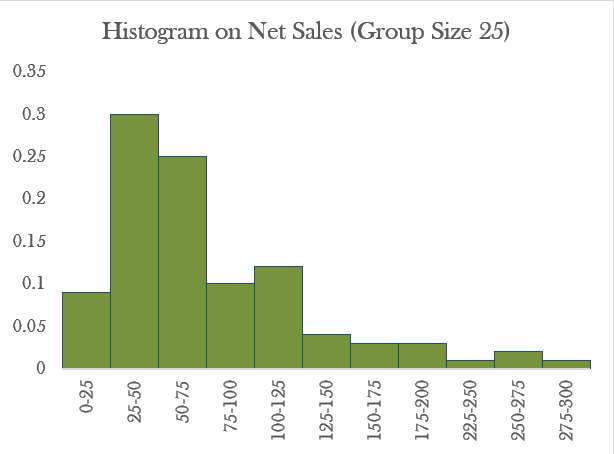
\includegraphics[scale=0.5]{images/ch2Histogram.png}
\end{center}

\begin{center}
\textit{We can visually identify the point where the most observations are \textbf{concentrated} (aka. central tendency), and the pattern of the \textbf{spread} (aka. variability).  
}
\end{center}

\end{frame}


\begin{frame}{Summarizing One Continuous Variable - Histogram (5/5)}

\begin{center}
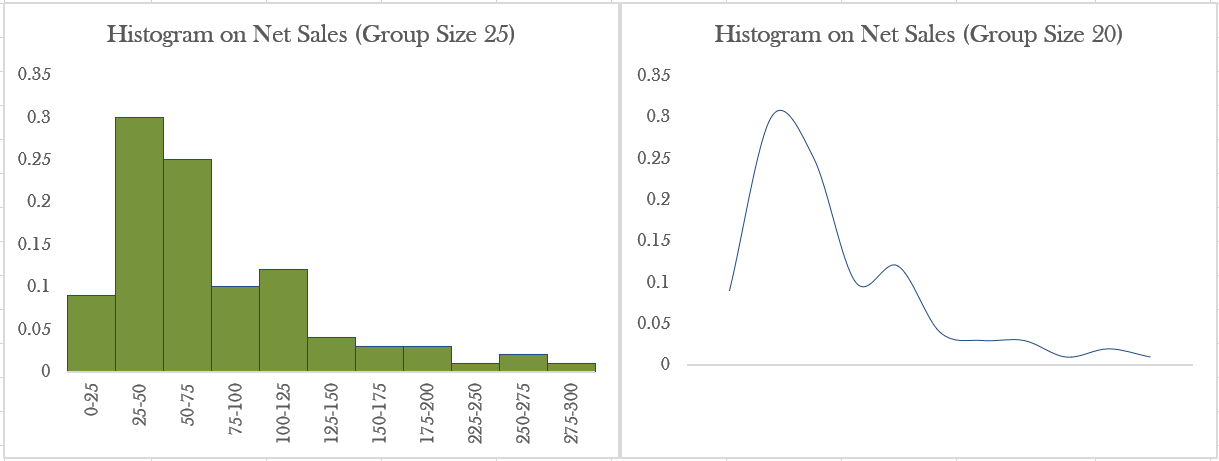
\includegraphics[scale=0.33]{images/ch2Histogram5.png}
\end{center}

\begin{center}
\textit{We can also attempt to simplify its appearance by drawing a fit line.}

\begin{scriptsize}
\textit{ 
If we assume the total area under the fit line is the same with the histogram, we can borrow calculus to obtain the proportion of a sub-group (Note: Don't worry! No one knows what that means at this point!!!).
}
\end{scriptsize}

\end{center}

\end{frame}

\subsubsection{Scatter Plot}
\begin{frame}{Visualizing the Relations Between Two Variables - Scatter Plot}

\begin{center}
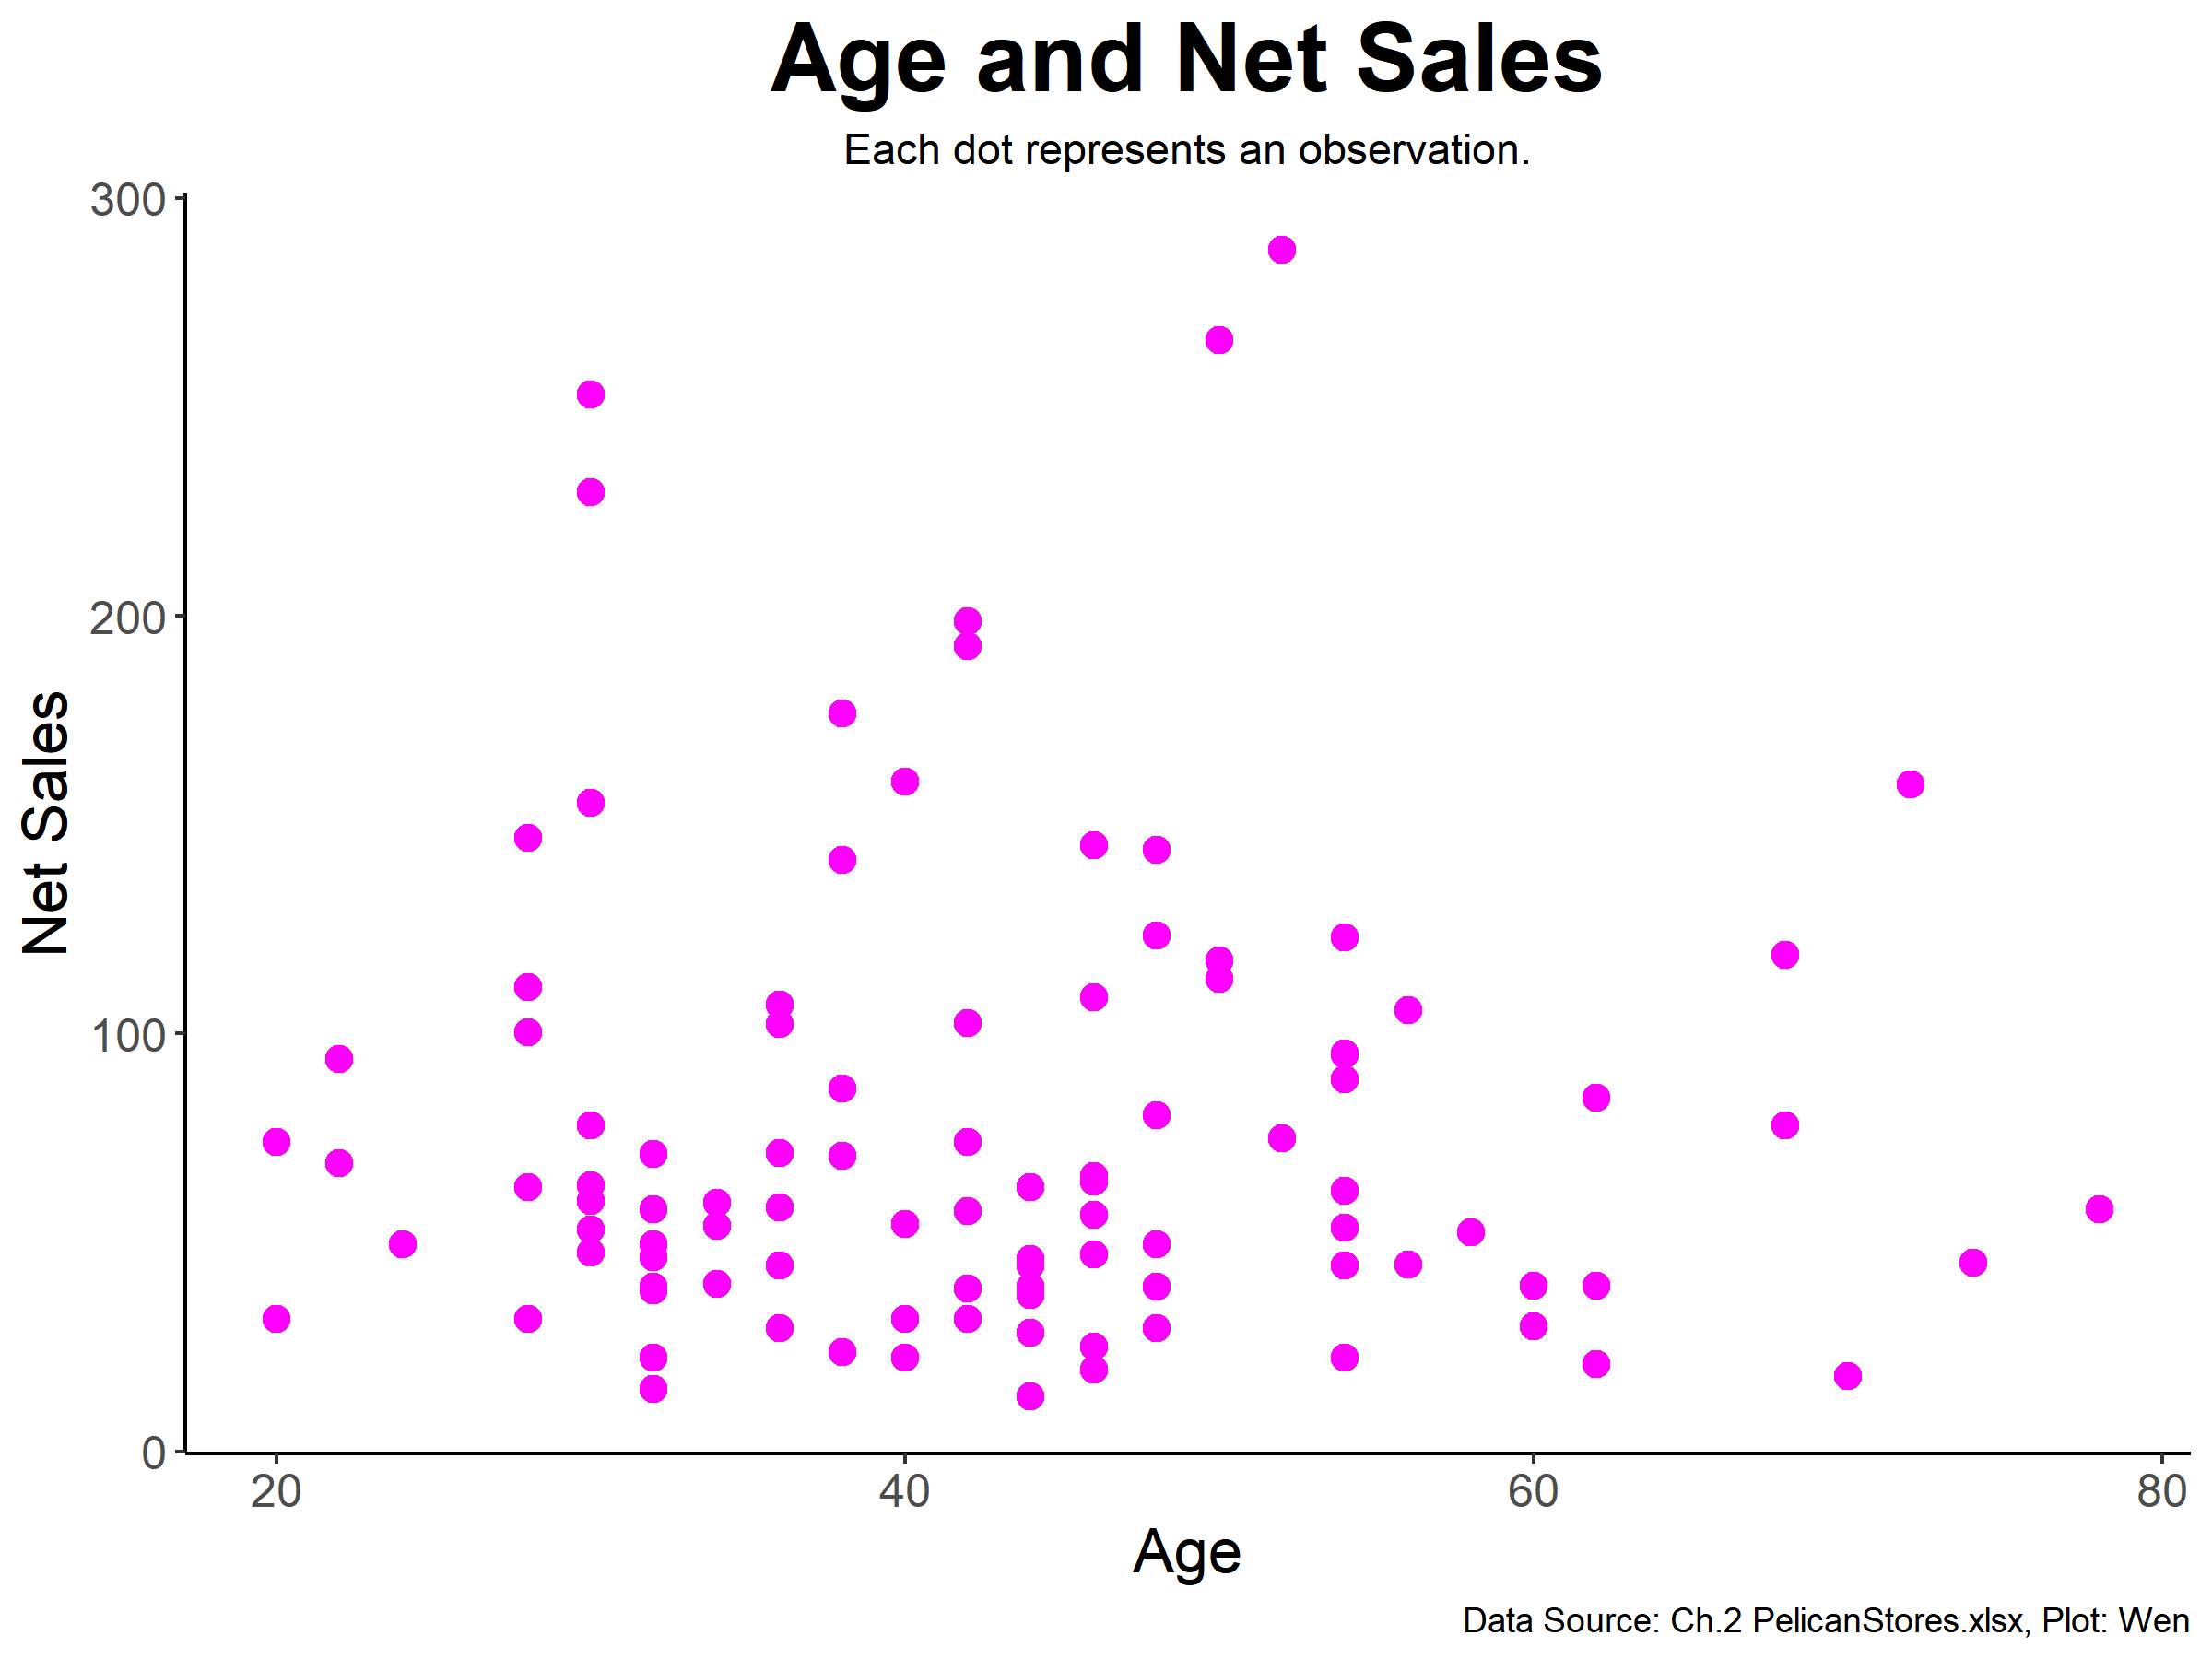
\includegraphics[scale=0.45]{images/ch2AgeNetSales.png}

\end{center}
\end{frame}

\begin{frame}{Visualizing the Relations Between Two Variables - Scatter Plot (cont.)}

\begin{center}
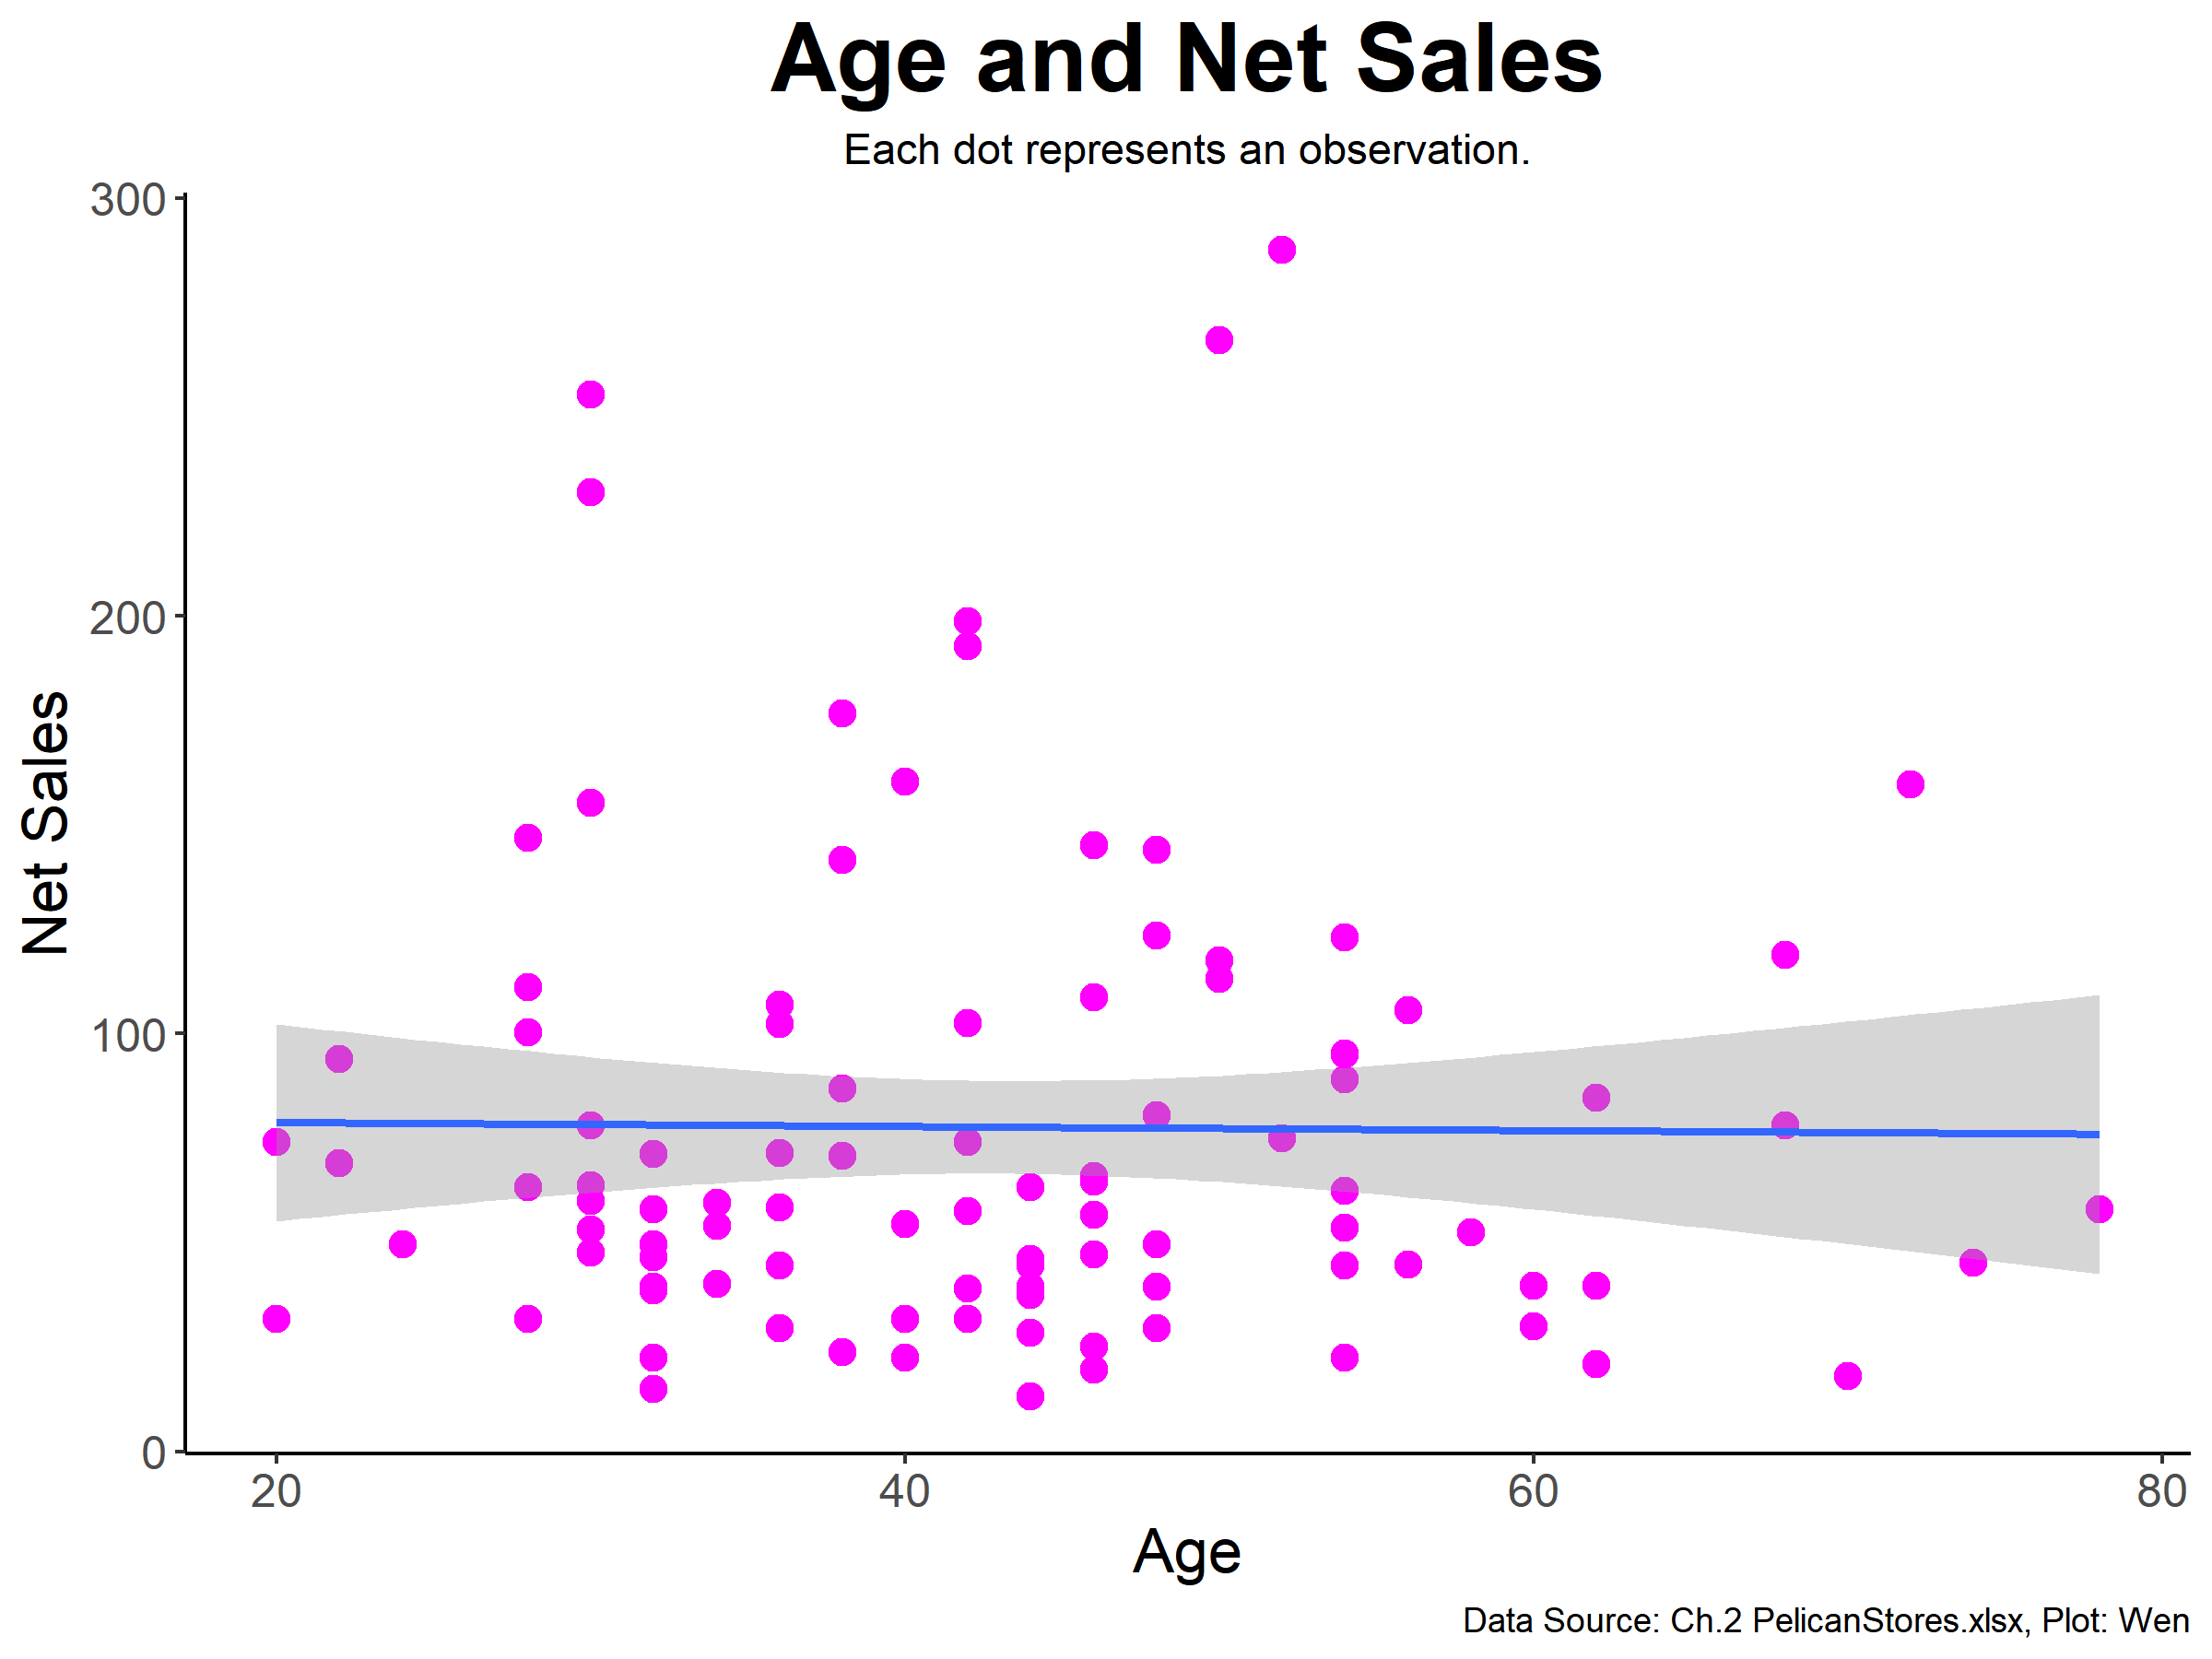
\includegraphics[scale=0.35]{images/ch2AgeNetSalesRegression.png}

Based on the scatter plot, we can identify a line (regression line) that can represent the relationship between the two variables.
$$\textsf{Net Sales} = 79.6592 -0.0478 \cdot \textsf{Age}$$
\end{center}
\end{frame}


\begin{frame}{Check Your Understanding}
\vspace{0.2 cm}
How would you evaluate the relationship between the following two variables? Can you identify the regression line? 

\begin{center}
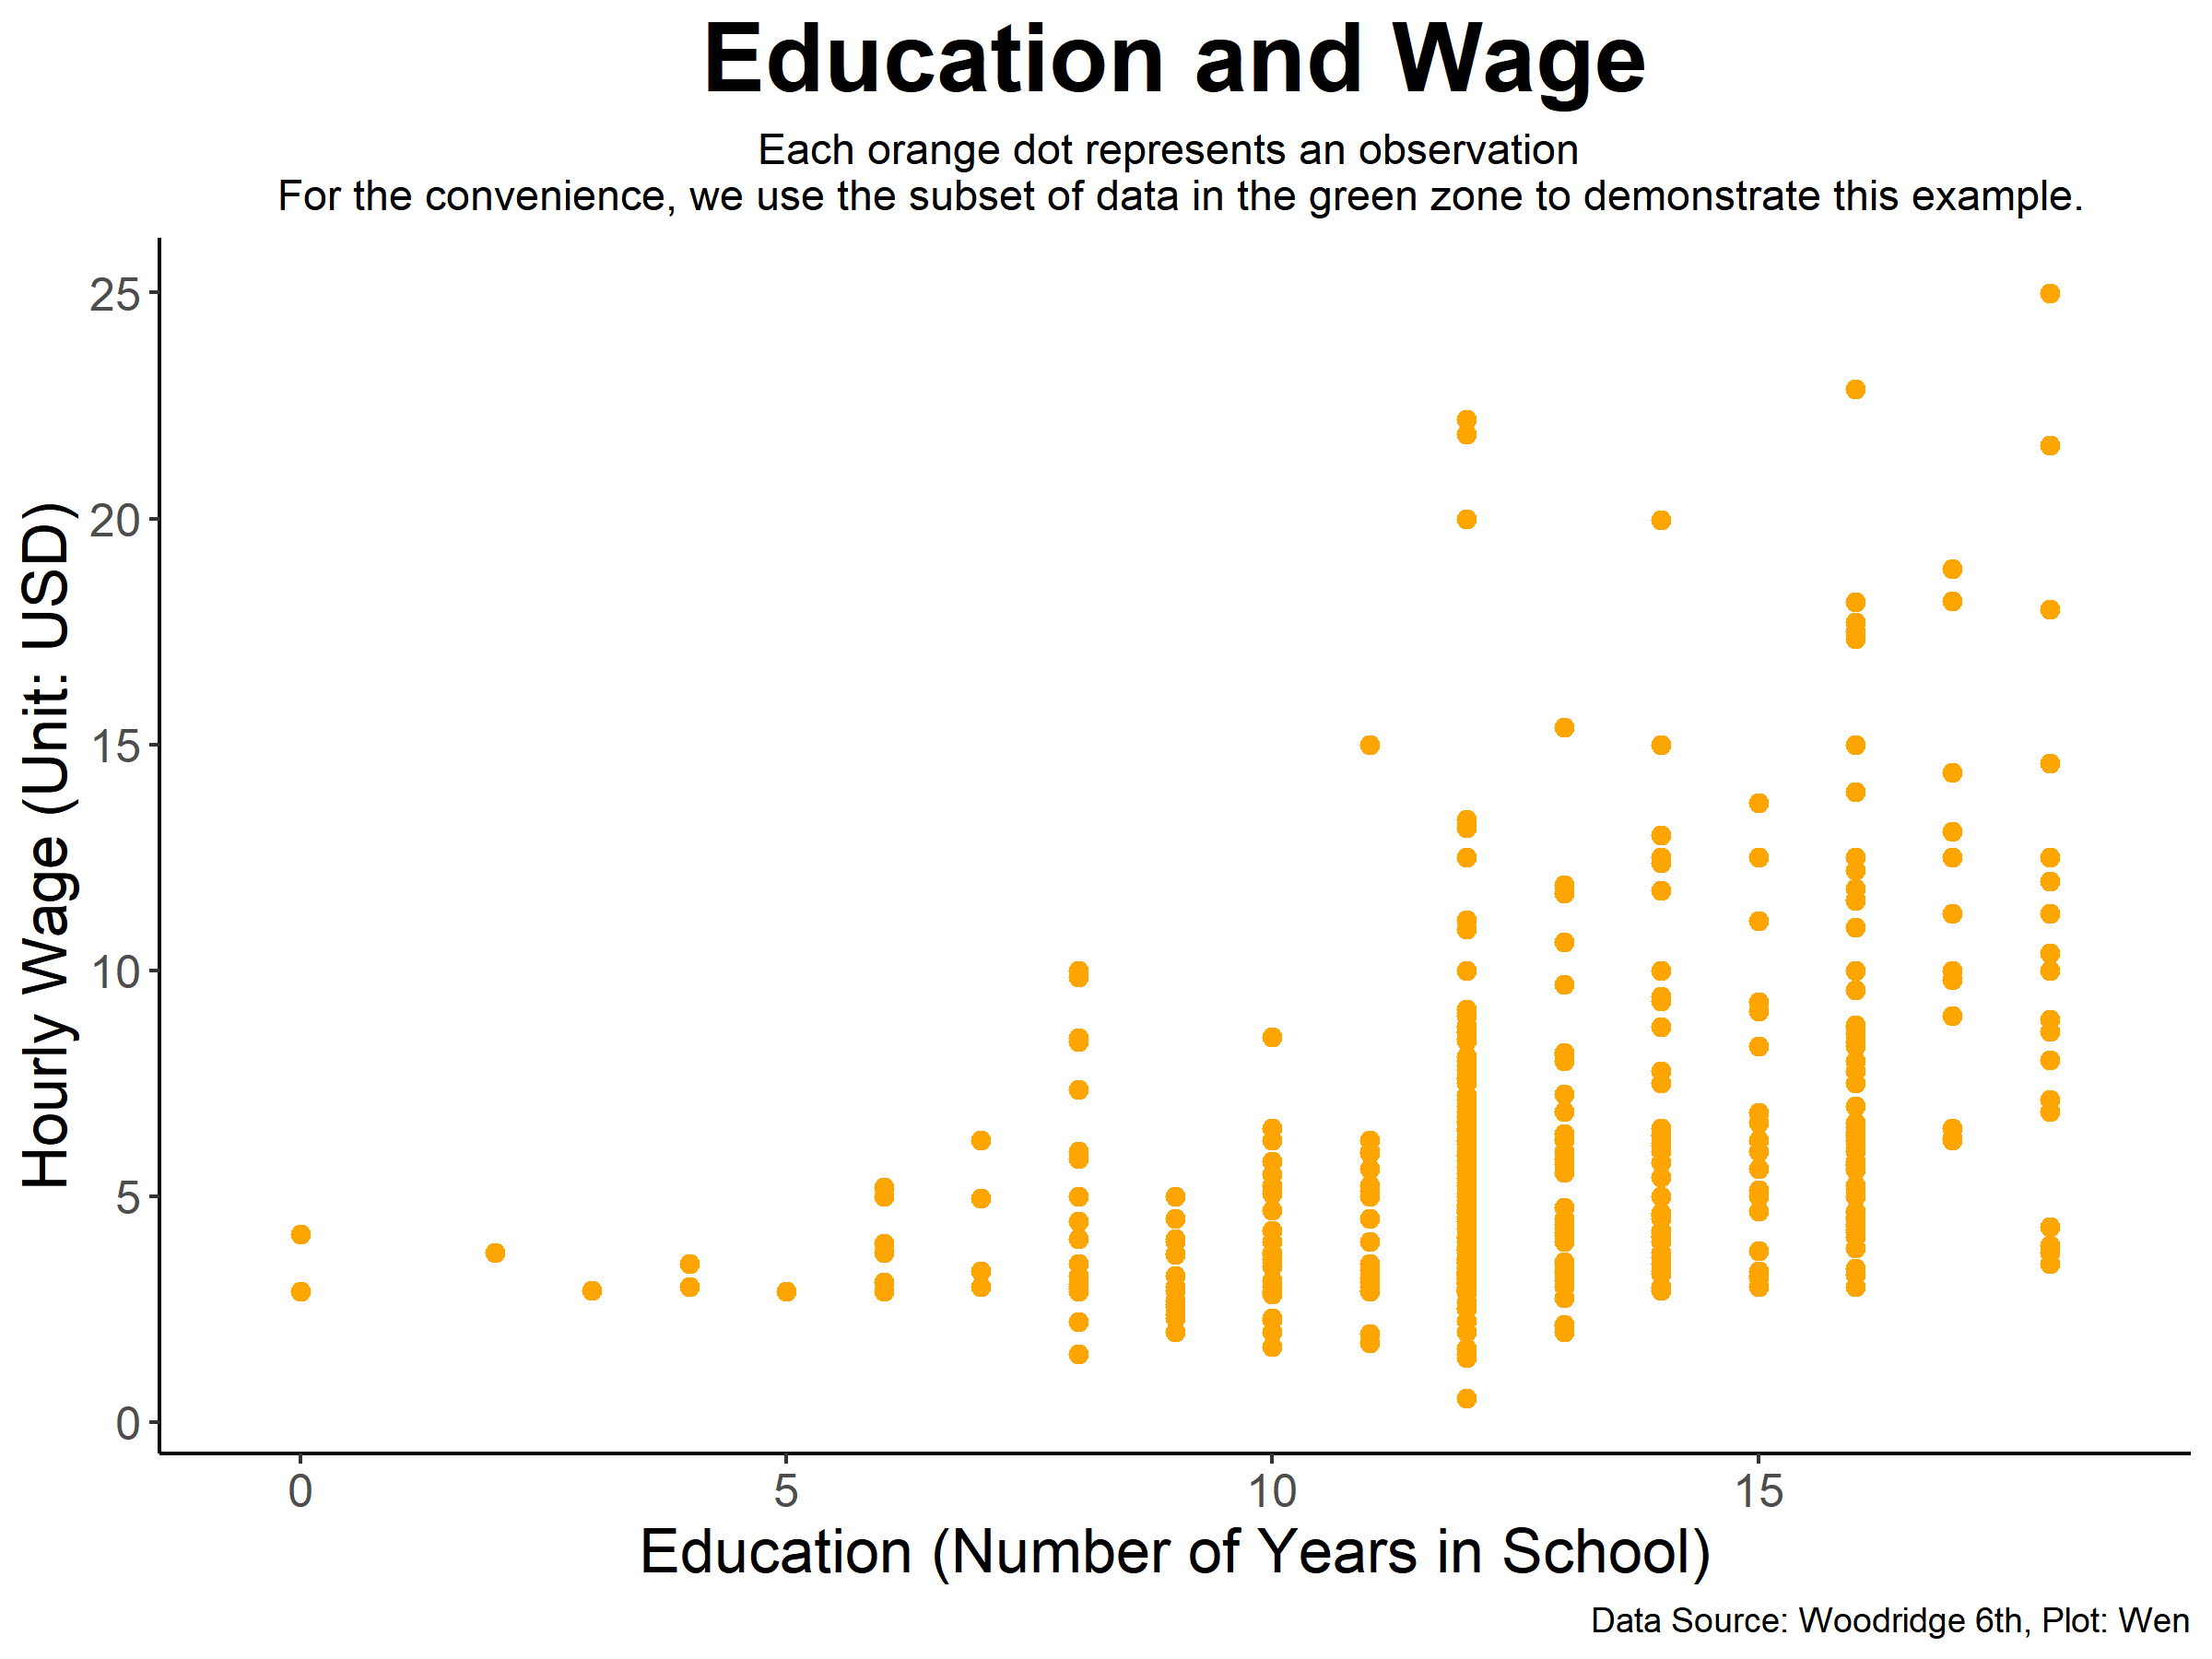
\includegraphics[scale=0.45]{images/plotCorrelations.png}
\end{center}

\end{frame}

\subsubsection{Frequency Analysis}
\begin{frame}{Frequency Analysis for Two Qualitative Variables}

\begin{center}
Cross-tabulating the \textit{Payment Method} against the\textit{Type of Customers}

\end{center}
\begin{multicols}{2}
\begin{center}
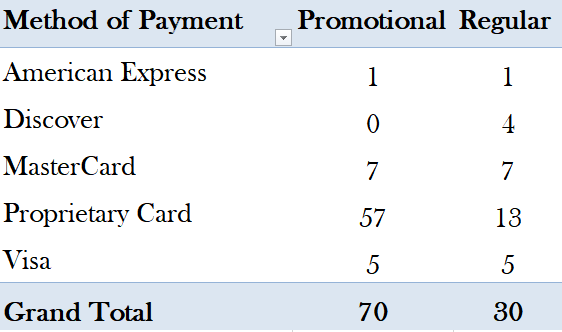
\includegraphics[scale=0.4]{images/ch2CrossTabQulitative.png}

\textit{What do you see from the results? 
}

\end{center}

\begin{center}

\vspace{3cm}
\begin{scriptsize}
\textit{Excel Pivot Table Implementation
}
\end{scriptsize}

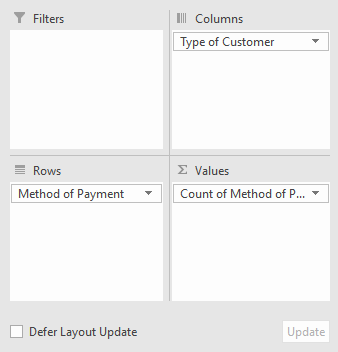
\includegraphics[scale=0.4]{images/ch2CrossTabQulitativePivot.png}
\end{center}

\end{multicols}


\end{frame}


\begin{frame}{Frequency Analysis for One Qualitative and One Continuous Variable}

\begin{center}
Cross-tabulating the \textit{Payment Method} against the \textit{Net Sales}

\vspace{0.3 cm}

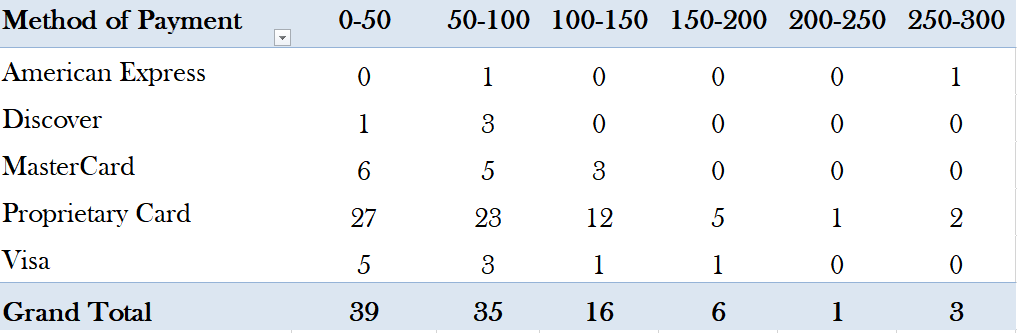
\includegraphics[scale=0.4]{images/ch2CrossTabQualitativeContinuous.png}

\vspace{0.5 cm}

\textit{What do you see from the results?}

\end{center}



\end{frame}

\begin{frame}{Frequency Analysis for Two Continuous Variable}


\begin{center}
Cross-tabulating the \textit{Age} against the \textit{Net Sales}

\vspace{0.3 cm}

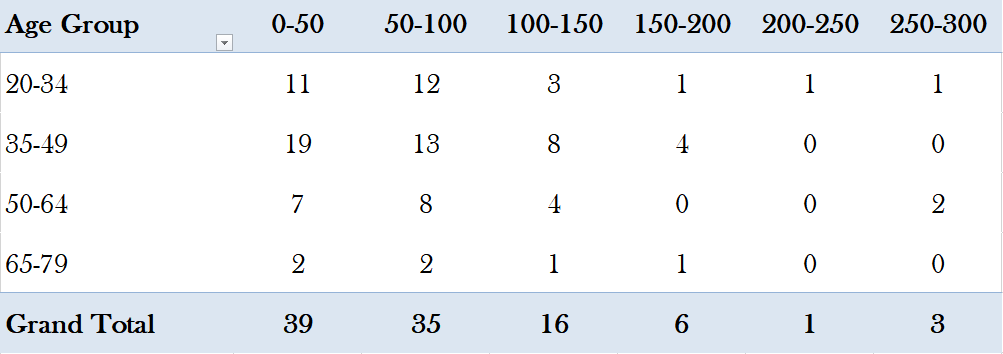
\includegraphics[scale=0.4]{images/ch2CrossTabContinuous.png}

\vspace{0.5 cm}

\textit{What do you see from the results?}

\end{center}


\end{frame}



\begin{frame}{Check Your Understanding 1/5}

A frequency distribution is
\begin{itemize}
\item a. a tabular summary of a data set showing the relative frequency
\item b. a graphical form of representing data
\item c. a tabular summary of a data set showing the frequency of items in each of several non-overlapping classes
\item d. a graphical device for presenting qualitative data

\end{itemize}
\end{frame}


\begin{frame}{Check Your Understanding 2/5}

The sum of the relative frequencies for all classes will always equal
\begin{itemize}
\item a.	the sample size
\item b.	the number of classes
\item c.	one
\item d.	any value greater than one

\end{itemize}
\end{frame}

\begin{frame}{Check Your Understanding 3/5}

In constructing a frequency distribution for quantitative data, the approximate class width is computed as
\begin{itemize}
\item a.	(largest data value - smallest data value)/(number of classes)
\item b.	(largest data value - smallest data value)/(sample size)
\item c.	(smallest data value - largest data value)/(sample size)
\item d.	(largest data value)/(number of classes)

\end{itemize}
\end{frame}


\begin{frame}{Check Your Understanding 4/5}

\begin{center}
The Numbers of Hours Worked (n = 400)
\vspace{0.2 cm}

\begin{tabular}{c|c}
\hline 
Number of Hours & Frequency \\ 
\hline 
0 - 9 & 20 \\ 
\hline 
10 - 19 & 80 \\ 
\hline 
20 - 29 & 200 \\ 
\hline 
30 - 39 & 100 \\ 
\hline 
\end{tabular} 
\end{center}

Refer to the frequency distribution above, the proportion (fraction) of people working 19 hours or less is

\begin{itemize}
\item a.	100
\item b.	0.25
\item c.	0.95
\item d.	0.05

\end{itemize}
\end{frame}


\begin{frame}{Check Your Understanding 5/5}

\begin{center}
The Numbers of Hours Worked (n = 400)
\vspace{0.2 cm}

\begin{tabular}{c|c}
\hline 
Number of Hours & Frequency \\ 
\hline 
0 - 9 & 20 \\ 
\hline 
10 - 19 & 80 \\ 
\hline 
20 - 29 & 200 \\ 
\hline 
30 - 39 & 100 \\ 
\hline 
\end{tabular} 
\end{center}

Refer to the frequency distribution above, the cumulative relative frequency for the 20 – 29 class is

\begin{itemize}
\item a.	is 300
\item b.	is 0.25
\item c.	is 0.75
\item d.	is 0.5

\end{itemize}
\end{frame}


\begin{frame}{Check Your Understanding: Bonus}
\begin{center}
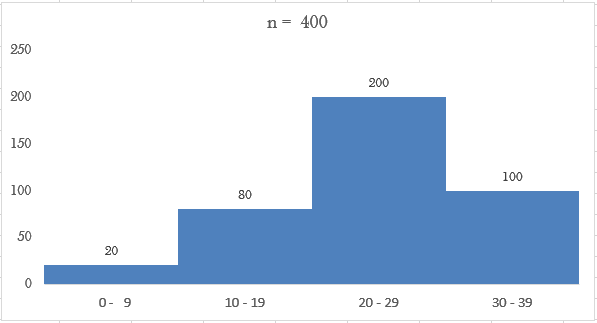
\includegraphics[scale=0.5]{images/ch2CheckYourUnderstanding1.png}
\end{center}

Please identify the following section quickly. 
\begin{itemize}
\item Greater than 9
\item Less than 19
\item Greater than 10 but less than 29
\item Equal to 30
\end{itemize}

\end{frame}


\subsection{Section 2. Numerical Measures}

\begin{frame}{Before the Numerical Measures - Review of Histogram}

\begin{center}

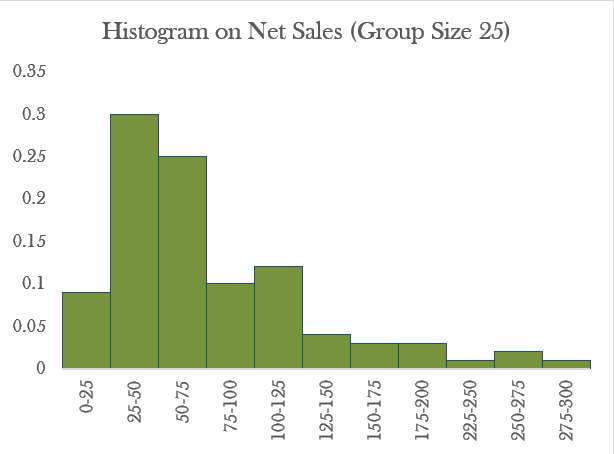
\includegraphics[scale=0.5]{images/ch2Histogram.png}
\end{center}

\begin{center}
\textit{We can visually identify the point where the most observations are \textbf{concentrated} (aka. central tendency), and the pattern of the \textbf{spread} (aka. variability).  
}
\end{center}

\end{frame}


\subsubsection{Mean and Median}
\begin{frame}{Numerical Measures: The Measures of Central Tendency}

\textbf{Mean} (aka. Mathematical Mean or Average)
$$\mu = \frac{\sum_{i=1}^{N}x_i}{N} \quad\text{or}\quad \bar{x} = \frac{\sum_{i=1}^{n}x_i}{n}$$

\begin{flushright}

\textit{Excel Formula: 
=AVERAGE(RANGE)
}
\end{flushright}



\textbf{Median}
$$ \text{The middle number} $$
$$ \textit{(when ranked from the lowest to the highest)} $$


\begin{flushright}

\textit{Excel Formula: 
=Median(RANGE)}

\end{flushright}



\end{frame}


\begin{frame}{Numerical Measures: The Measures of Central Tendency}
\begin{center}
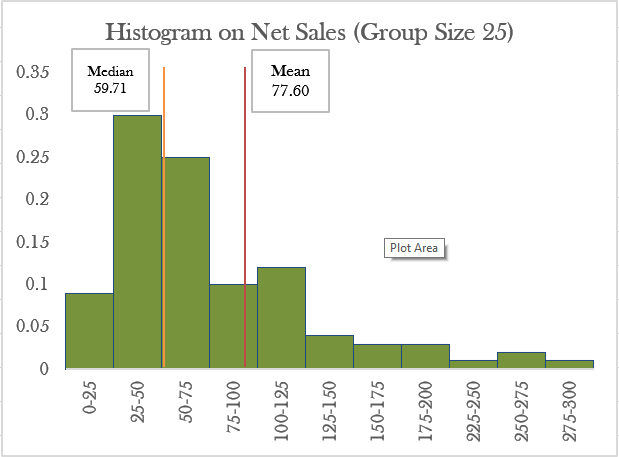
\includegraphics[scale=0.5]{images/ch2MeanMedian.png}

\textit{To represent the middle, the mean can be sensitive to the extreme values. Therefore, when extreme values are clearly present, we typically use median.}

\end{center}
\end{frame}






\subsubsection{Variance and S.D.}
\begin{frame}{Numerical Measures: The Measures of Variability}
\textbf{Range}
$$range = max(x_i) - min(x_i)$$

\begin{flushright}

\textit{Excel Formula: 
=Max(RANGE)-Min(RANGE)}

\end{flushright}


\textbf{Variance}
$$  \sigma^2 = \frac{\sum_{i=1}^N(x_i - \mu)^2}{N} \quad\text{or}\quad  s^2 = \frac{\sum_{i=1}^n(x_i - \bar{x})^2}{n-1}  $$

\begin{flushright}

\textit{Excel Formula: 
=Var.P(RANGE)}  or  \textit{=Var.S(RANGE)}

\end{flushright}


\textbf{Standard Deviation} (In short, s.d.)
$$ \sigma = \sqrt{\sigma^2} \quad\text{or}\quad s = \sqrt{s^2}$$

\begin{flushright}

\textit{Excel Formula: 
=Stdev.P(RANGE)} or \textit{=Stdev.S(RANGE)}

\end{flushright}


\end{frame}




\begin{frame}{The Measure of Variability Visualized}
\begin{center}

\textit{How would you comment on the level of spread that each group shows?}

\vspace{0.3 cm}

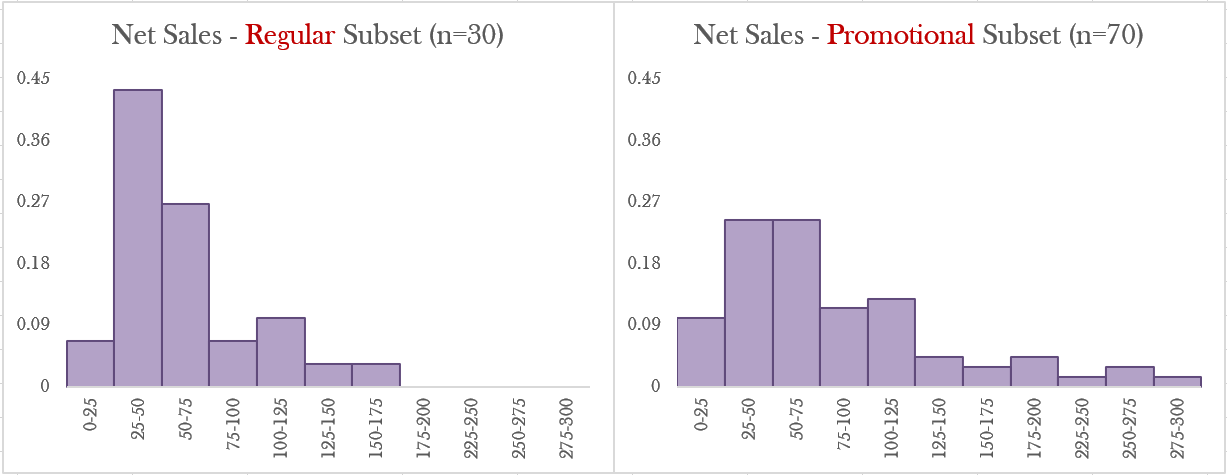
\includegraphics[scale=0.35]{images/ch2NetSalesVarianceTwoGroups.png}



\vspace{0.3 cm}

\begin{scriptsize}
\begin{tabular}{l|r|r|r|r|r}
\hline 
 & Mean & Median & Range & Variance & S.D. \\ 
\hline 
Regular & 61.992 & 51.000 & 137.250 & 1,229.761 & 35.068 \\ 
\hline 
Promotional & 84.290 & 63.420 & 274.360 & 3,777.614 & 61.462 \\ 
\hline 
\end{tabular} 
\end{scriptsize}

\end{center}
\end{frame}



\begin{frame}{Let's Get Closer to the Variance and S.D.}

Let's Think About the Meaning of the Variance 
$$  \sigma^2 = \frac{\sum_{i=1}^N(x_i - \mu)^2}{N} $$

Its numerator is some kind of calculation based on $\mu$:

$$  \sum_{i=1}^N(x_i - \mu)^2 $$

Its denominator divides the quantity above by the following number of chucks: 
$$ N $$

\end{frame}



\begin{frame}{Visualizing the Sum of Squares}
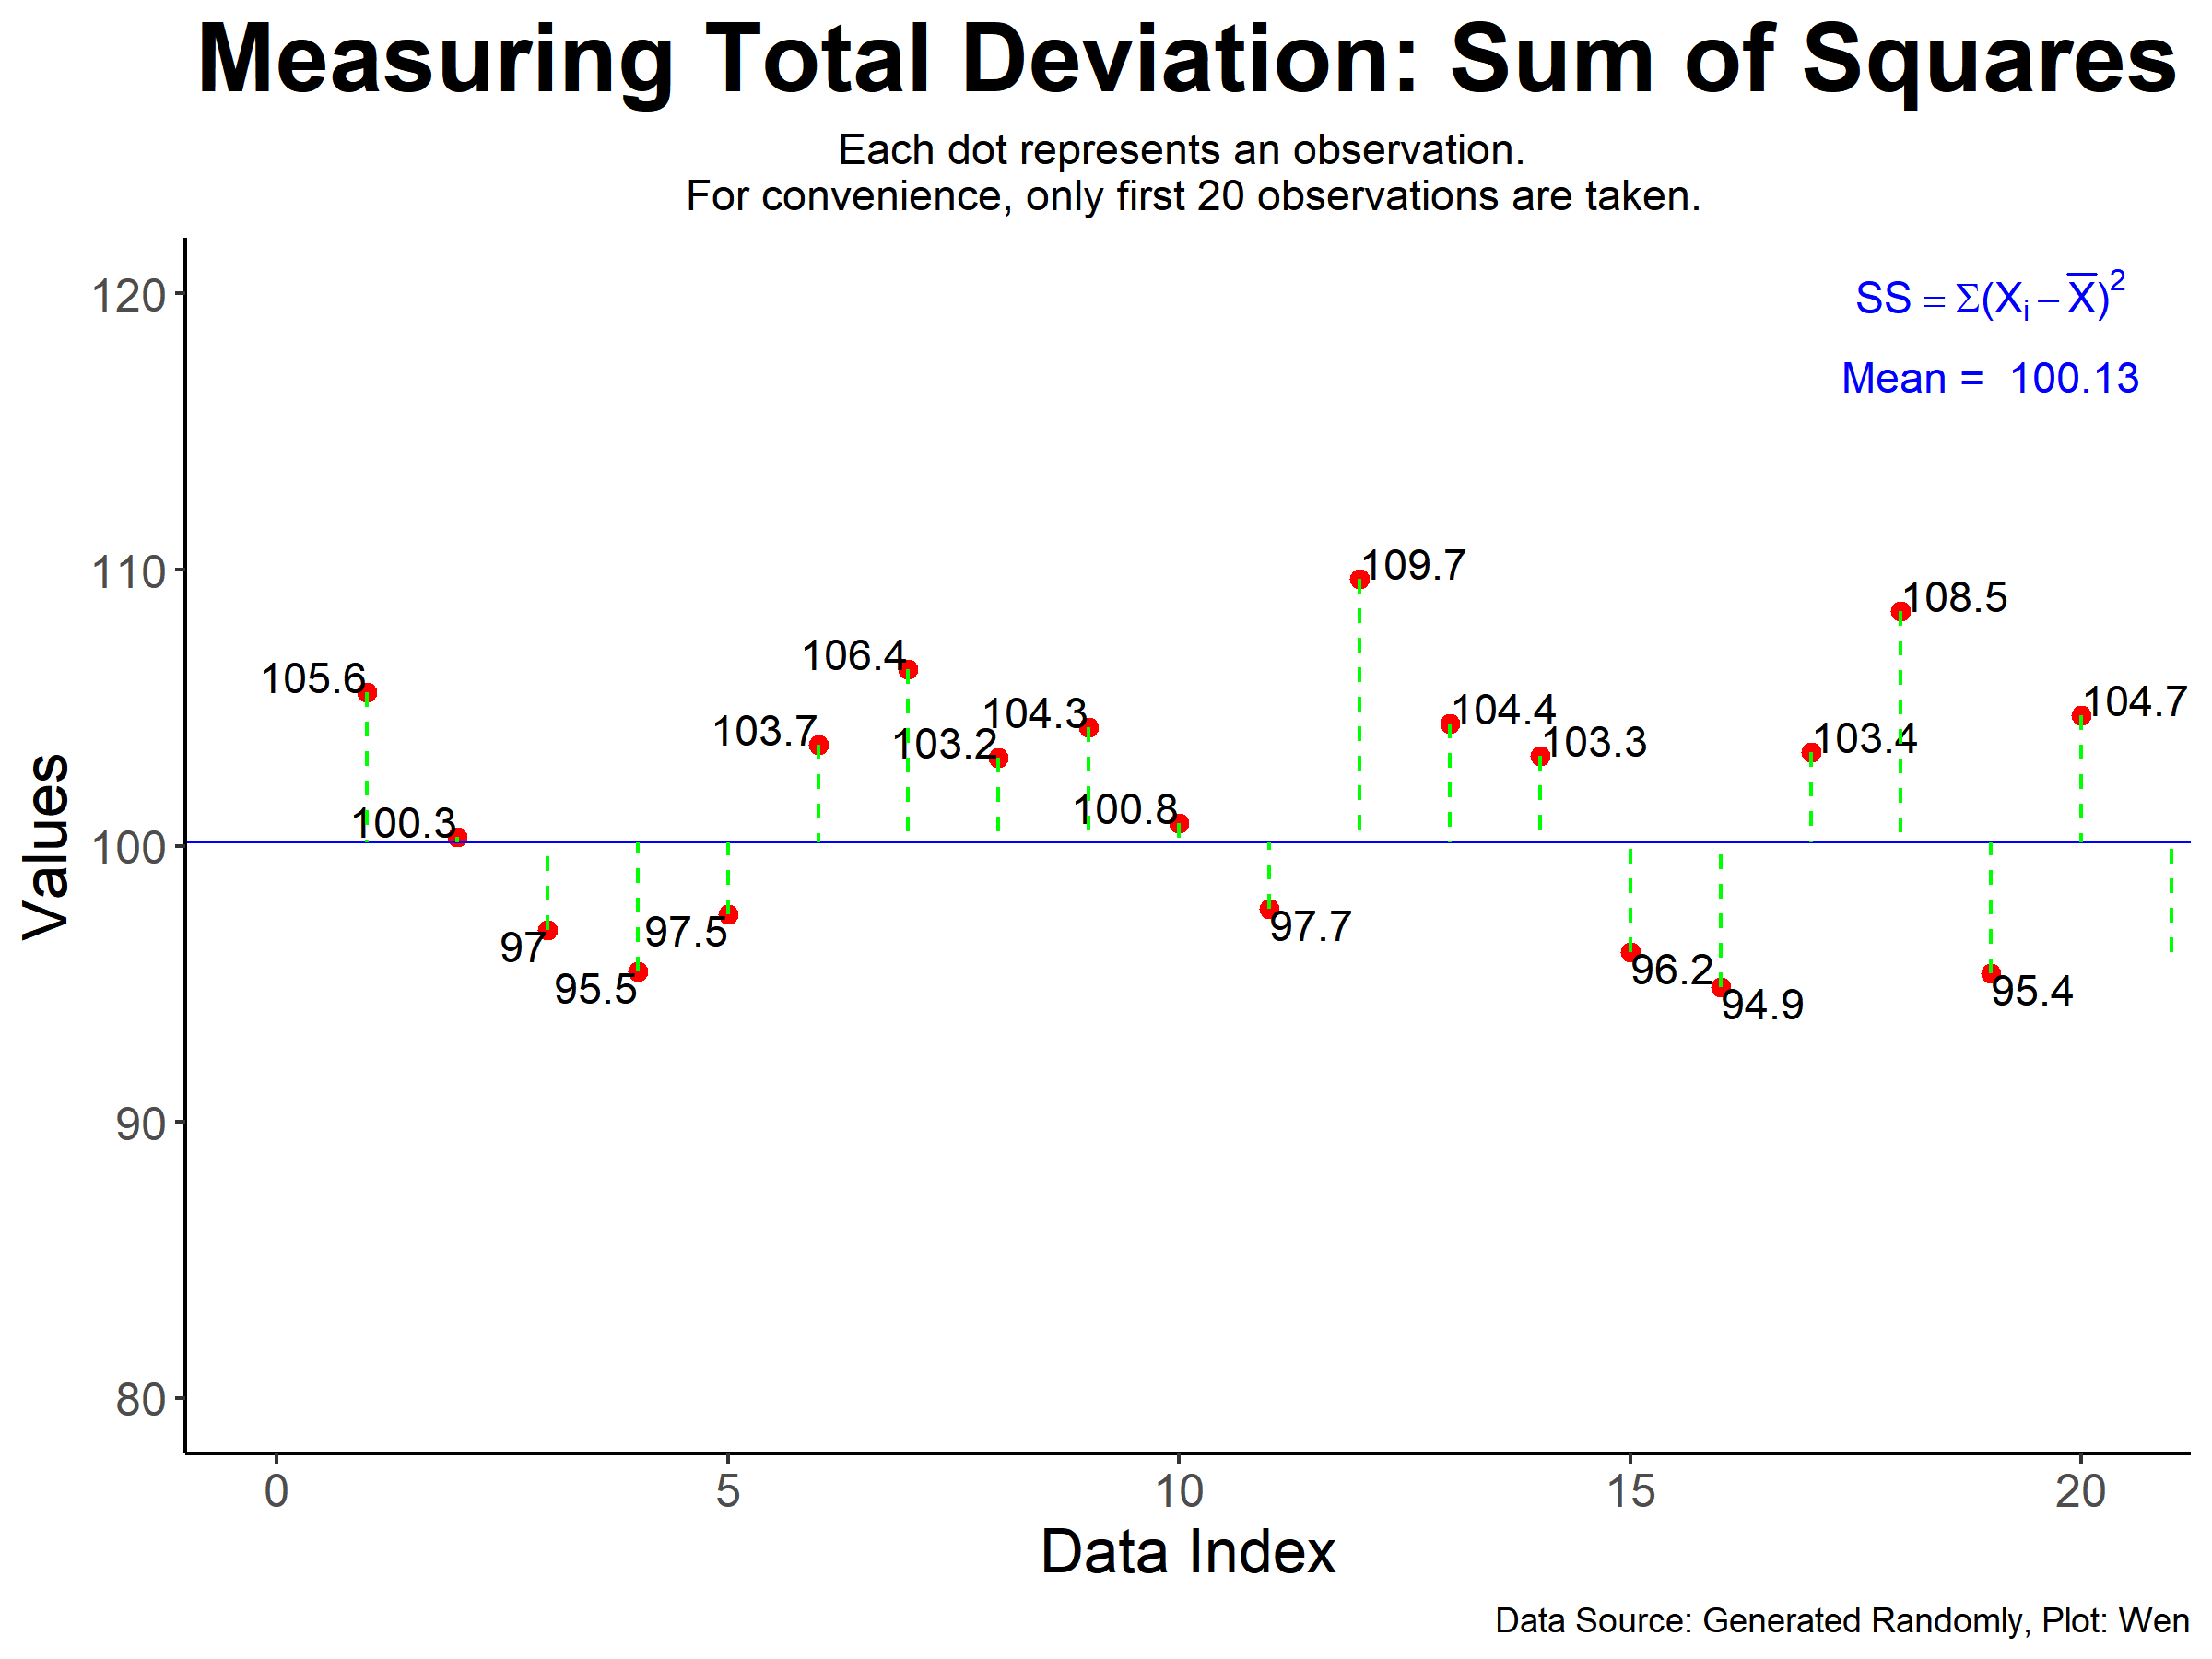
\includegraphics[scale=0.5]{images/uniScatterPlotAnnotated.png}
\end{frame}


\begin{frame}{Thinking about the Variance and Standard Deviation}

\begin{itemize}

\item Variance? Variation? Variability? What is the difference? 

\item What does the variance intended to measure? The extent of deviation of each point with respect to the mean of the data.

\item Why was the deviation squared before it was added together? $  \sum_{i=1}^N(x_i - \mu)^2 $ 

\item By square rooting the variance, the standard deviation is much easier to interpret because it maintains the same unit with the original data.

\item From the way they are calculated, they can never take negative values. When there is no variation in the data set, the variance will be 0, so is the s.d. 

\end{itemize}
\end{frame}


\begin{frame}{Check Your Understanding (1/2)}

The sum of deviations of the individual data values from their mean is
\begin{itemize}
\item a. always greater than zero
\item b. always less than zero
\item c. sometimes greater than and sometimes less than zero, depending on the data values
\item d. always equal to zero
\end{itemize}
\end{frame}


\begin{frame}{Check Your Understanding (2/2)}

Variable A has the variance of 4 and variable B has the s.d. of 2, then
\begin{itemize}
\item a. variable A has a greater variation
\item b. variable B has a greater variation
\item c. both have the same level of variation
\item d. not enough information
\end{itemize}
\end{frame}

\begin{frame}{Descriptive Statistics on Single Variable}
\begin{center}

\textit{Do you see how the descriptive statistics can be used to evaluate the data?}

\vspace{0.3 cm}

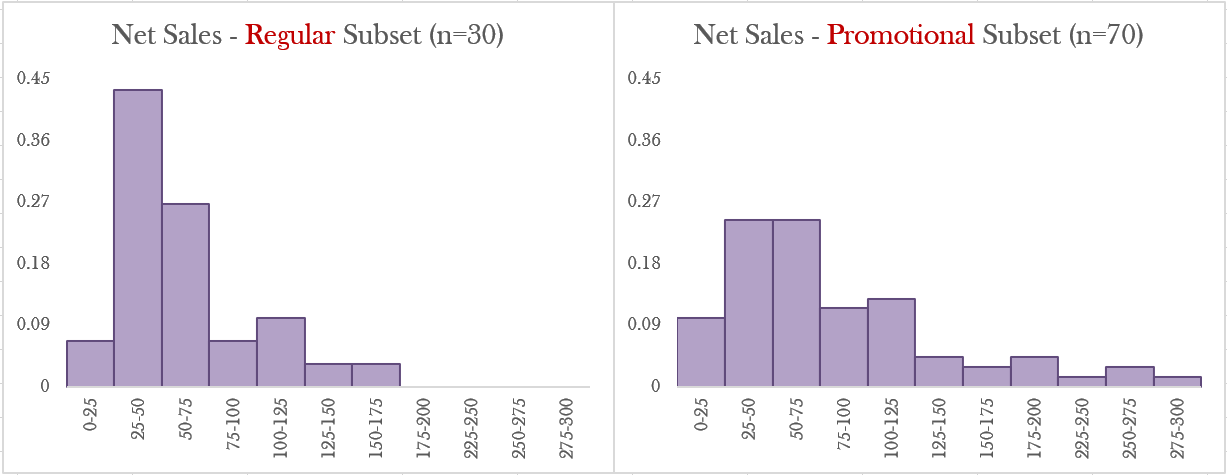
\includegraphics[scale=0.35]{images/ch2NetSalesVarianceTwoGroups.png}



\vspace{0.3 cm}

\begin{scriptsize}
\begin{tabular}{l|r|r|r|r|r}
\hline 
 & Mean & Median & Range & Variance & S.D. \\ 
\hline 
Regular & 61.992 & 51.000 & 137.250 & 1,229.761 & 35.068 \\ 
\hline 
Promotional & 84.290 & 63.420 & 274.360 & 3,777.614 & 61.462 \\ 
\hline 
\end{tabular} 
\end{scriptsize}

\end{center}
\end{frame}

\subsubsection{Relationship of Two Variables}
\begin{frame}{The Measures of Association Between Two Variables}
Oftentimes, we wish to measure and evaluate the relationship between two quantitative variables.\linebreak 

For example, we wish to determine the \textbf{direction} of the relationship: 
\begin{itemize}
\item When A increases, B also increases. (positively correlated)
\item When B increases, B decreases. (negatively correlated)
\item An increase in A has nothing to do with that in B. (no correlation)
\end{itemize}

We also wish to know how strong (\textbf{magnitude}) is such relationship.
\begin{itemize}
\item Always / almost always / in general / seldom / not at all
\item Very strong / strong / moderate / weak / very weak
\end{itemize}


\end{frame}

\begin{frame}{Using the Scatter Plot to Explore a Correlation}
\vspace{0.2 cm}
Do you observe a positive or a negative correlation between the education and the hourly wage? 

\begin{center}
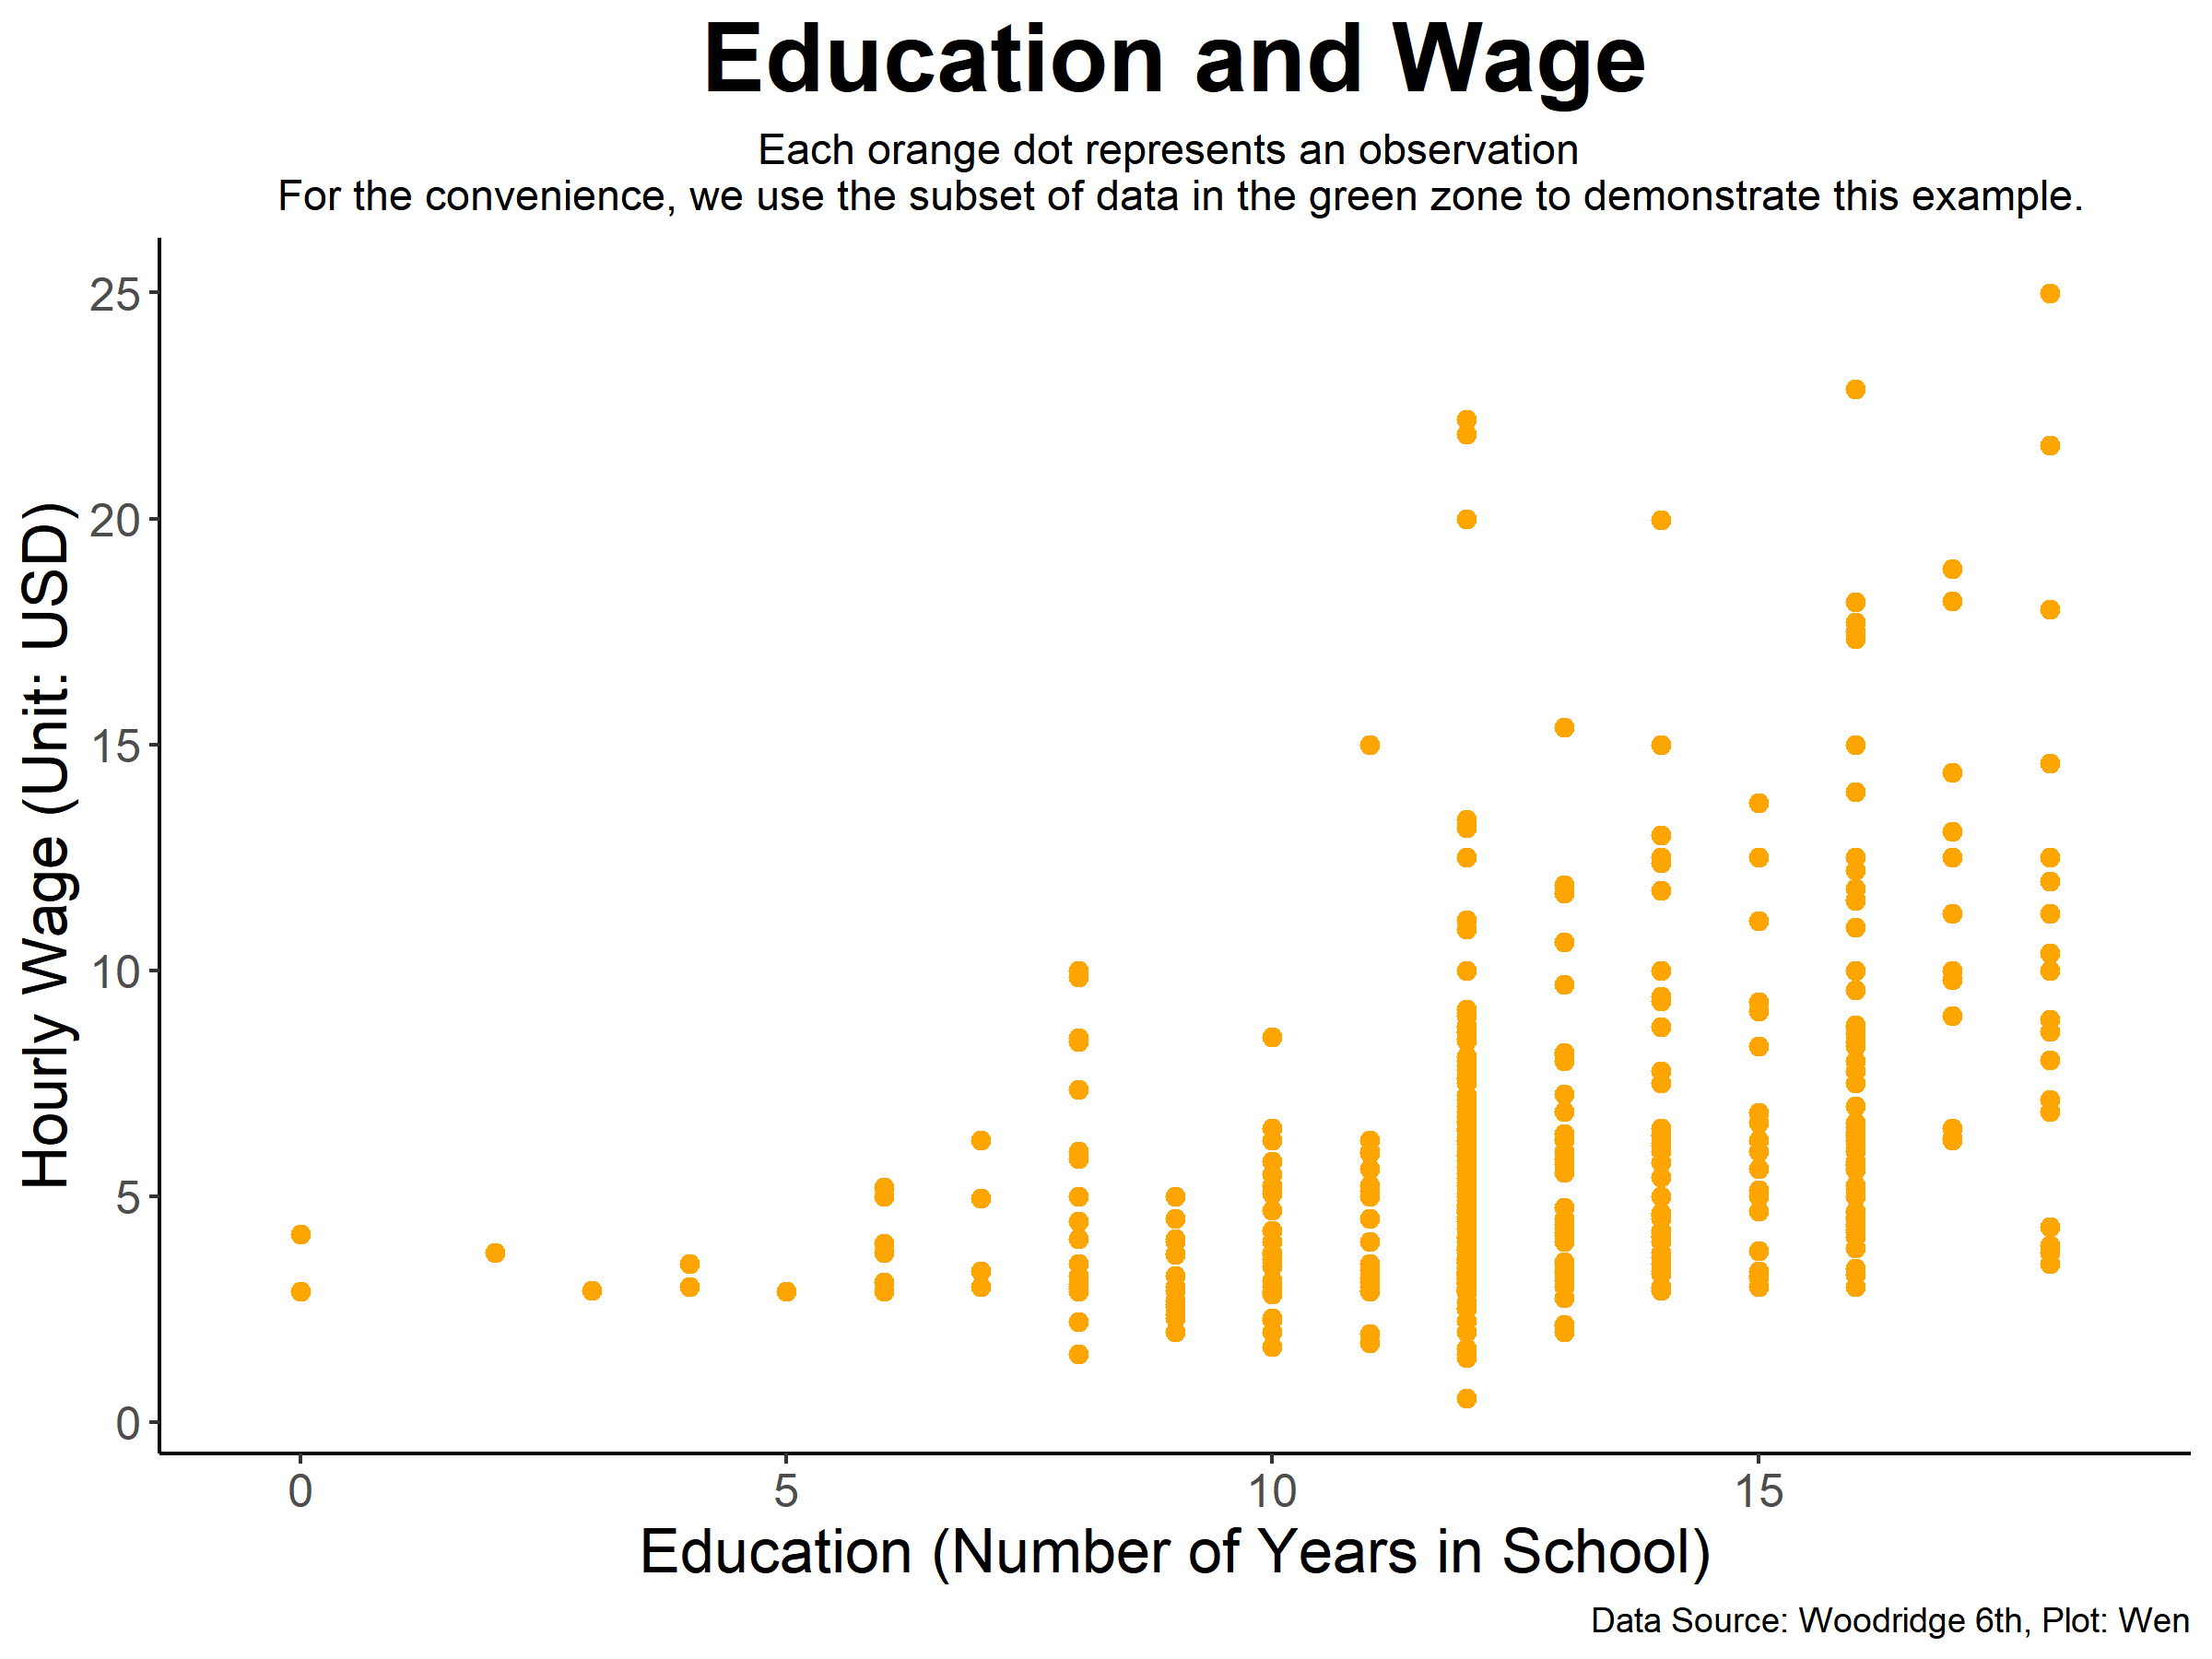
\includegraphics[scale=0.40]{images/plotCorrelations.png}
\end{center}

\end{frame}

\subsubsection{Covariance and Correlation Coefficient}
\begin{frame}{Numerical Measures of Correlation - Covariance}

\textbf{Covariance}

$$ \sigma_{xy} = \frac{\sum_{i=1}^{N}(x_i - \mu_x)(y_i - \mu_y)}{{N}} \quad\text{ or } $$
$$ s_{xy} = \frac{\sum_{i=1}^{N}(x_i - \bar{x})(y_i - \bar{y})}{{n - 1}} $$

\begin{flushright}
\textit{EXCEL Formula: =Covariance.P(var1\_Range, var2\_Range)}

\textit{EXCEL Formula: =Covariance.S(var1\_Range, var2\_Range)}
\end{flushright}


\end{frame}





\begin{frame}{Covariance Visualized (1/3)}
\vspace{0.2 cm}
We use the subset of the dataset (the green area) to illustrate the concept of the covariance.
\begin{center}
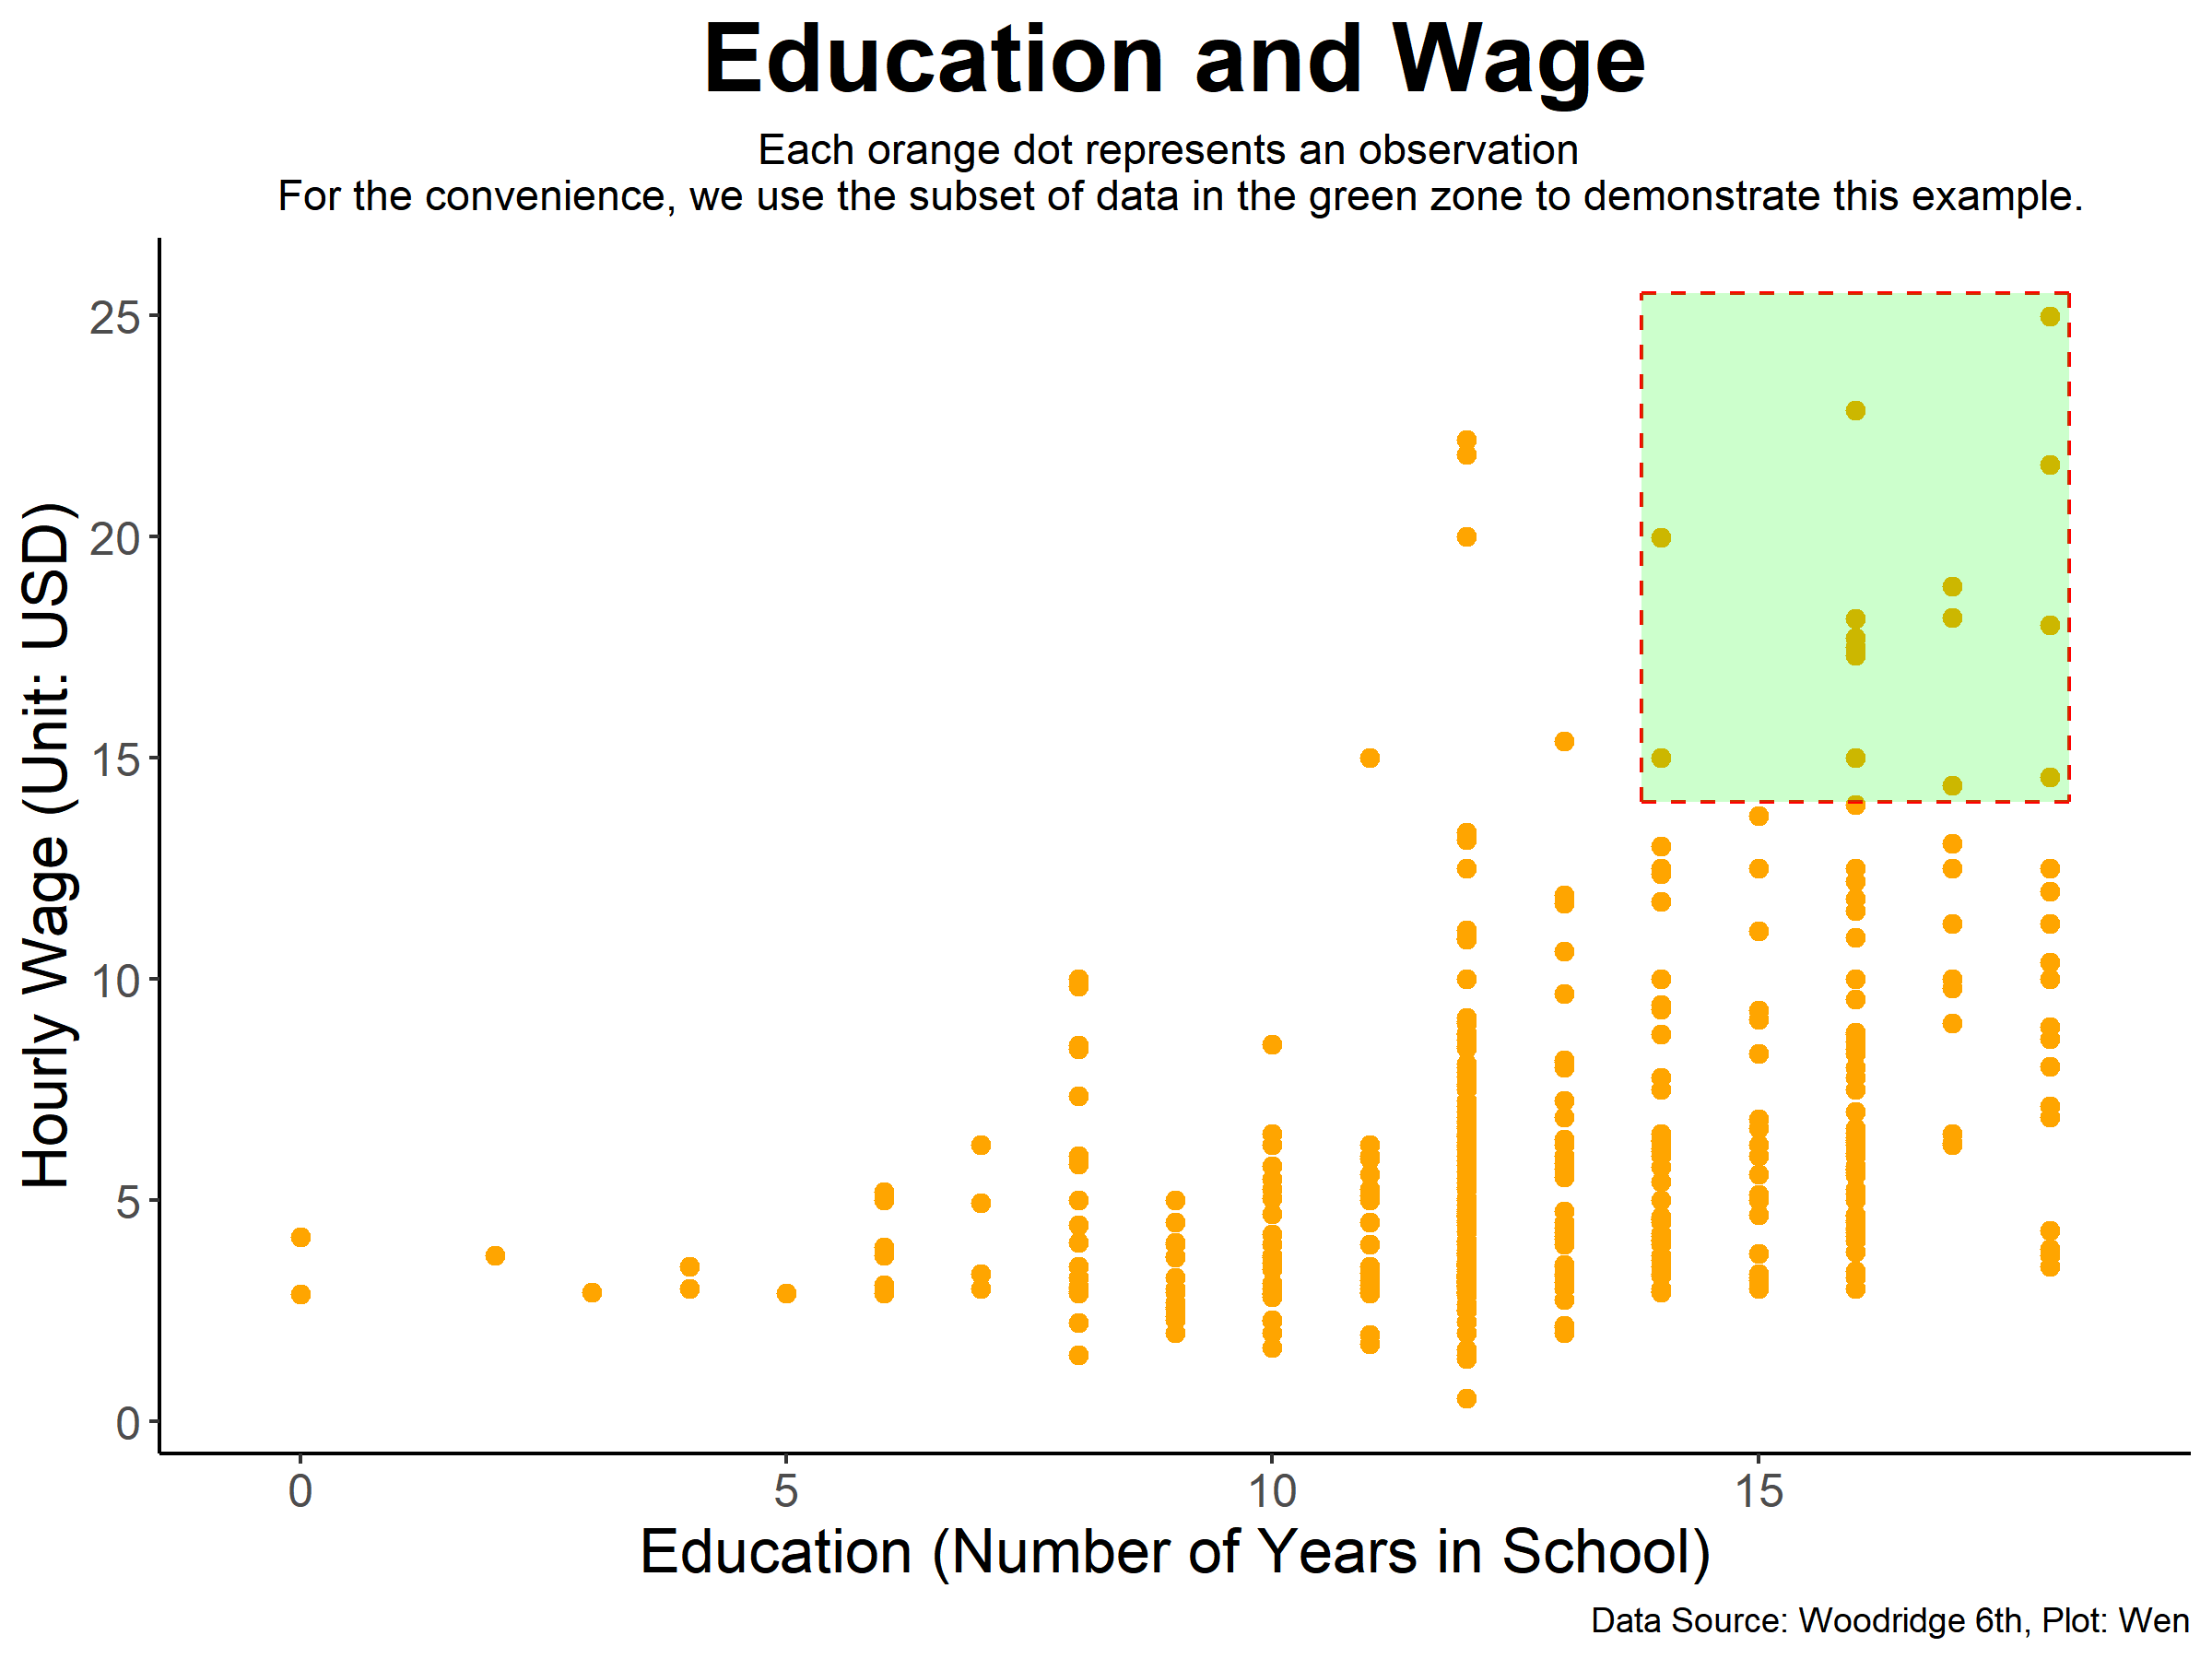
\includegraphics[scale=0.45]{images/plot0.png}
\end{center}

\end{frame}

\begin{frame}{Covariance Visualized (2/3)}
\vspace{0.2 cm}
\begin{center}
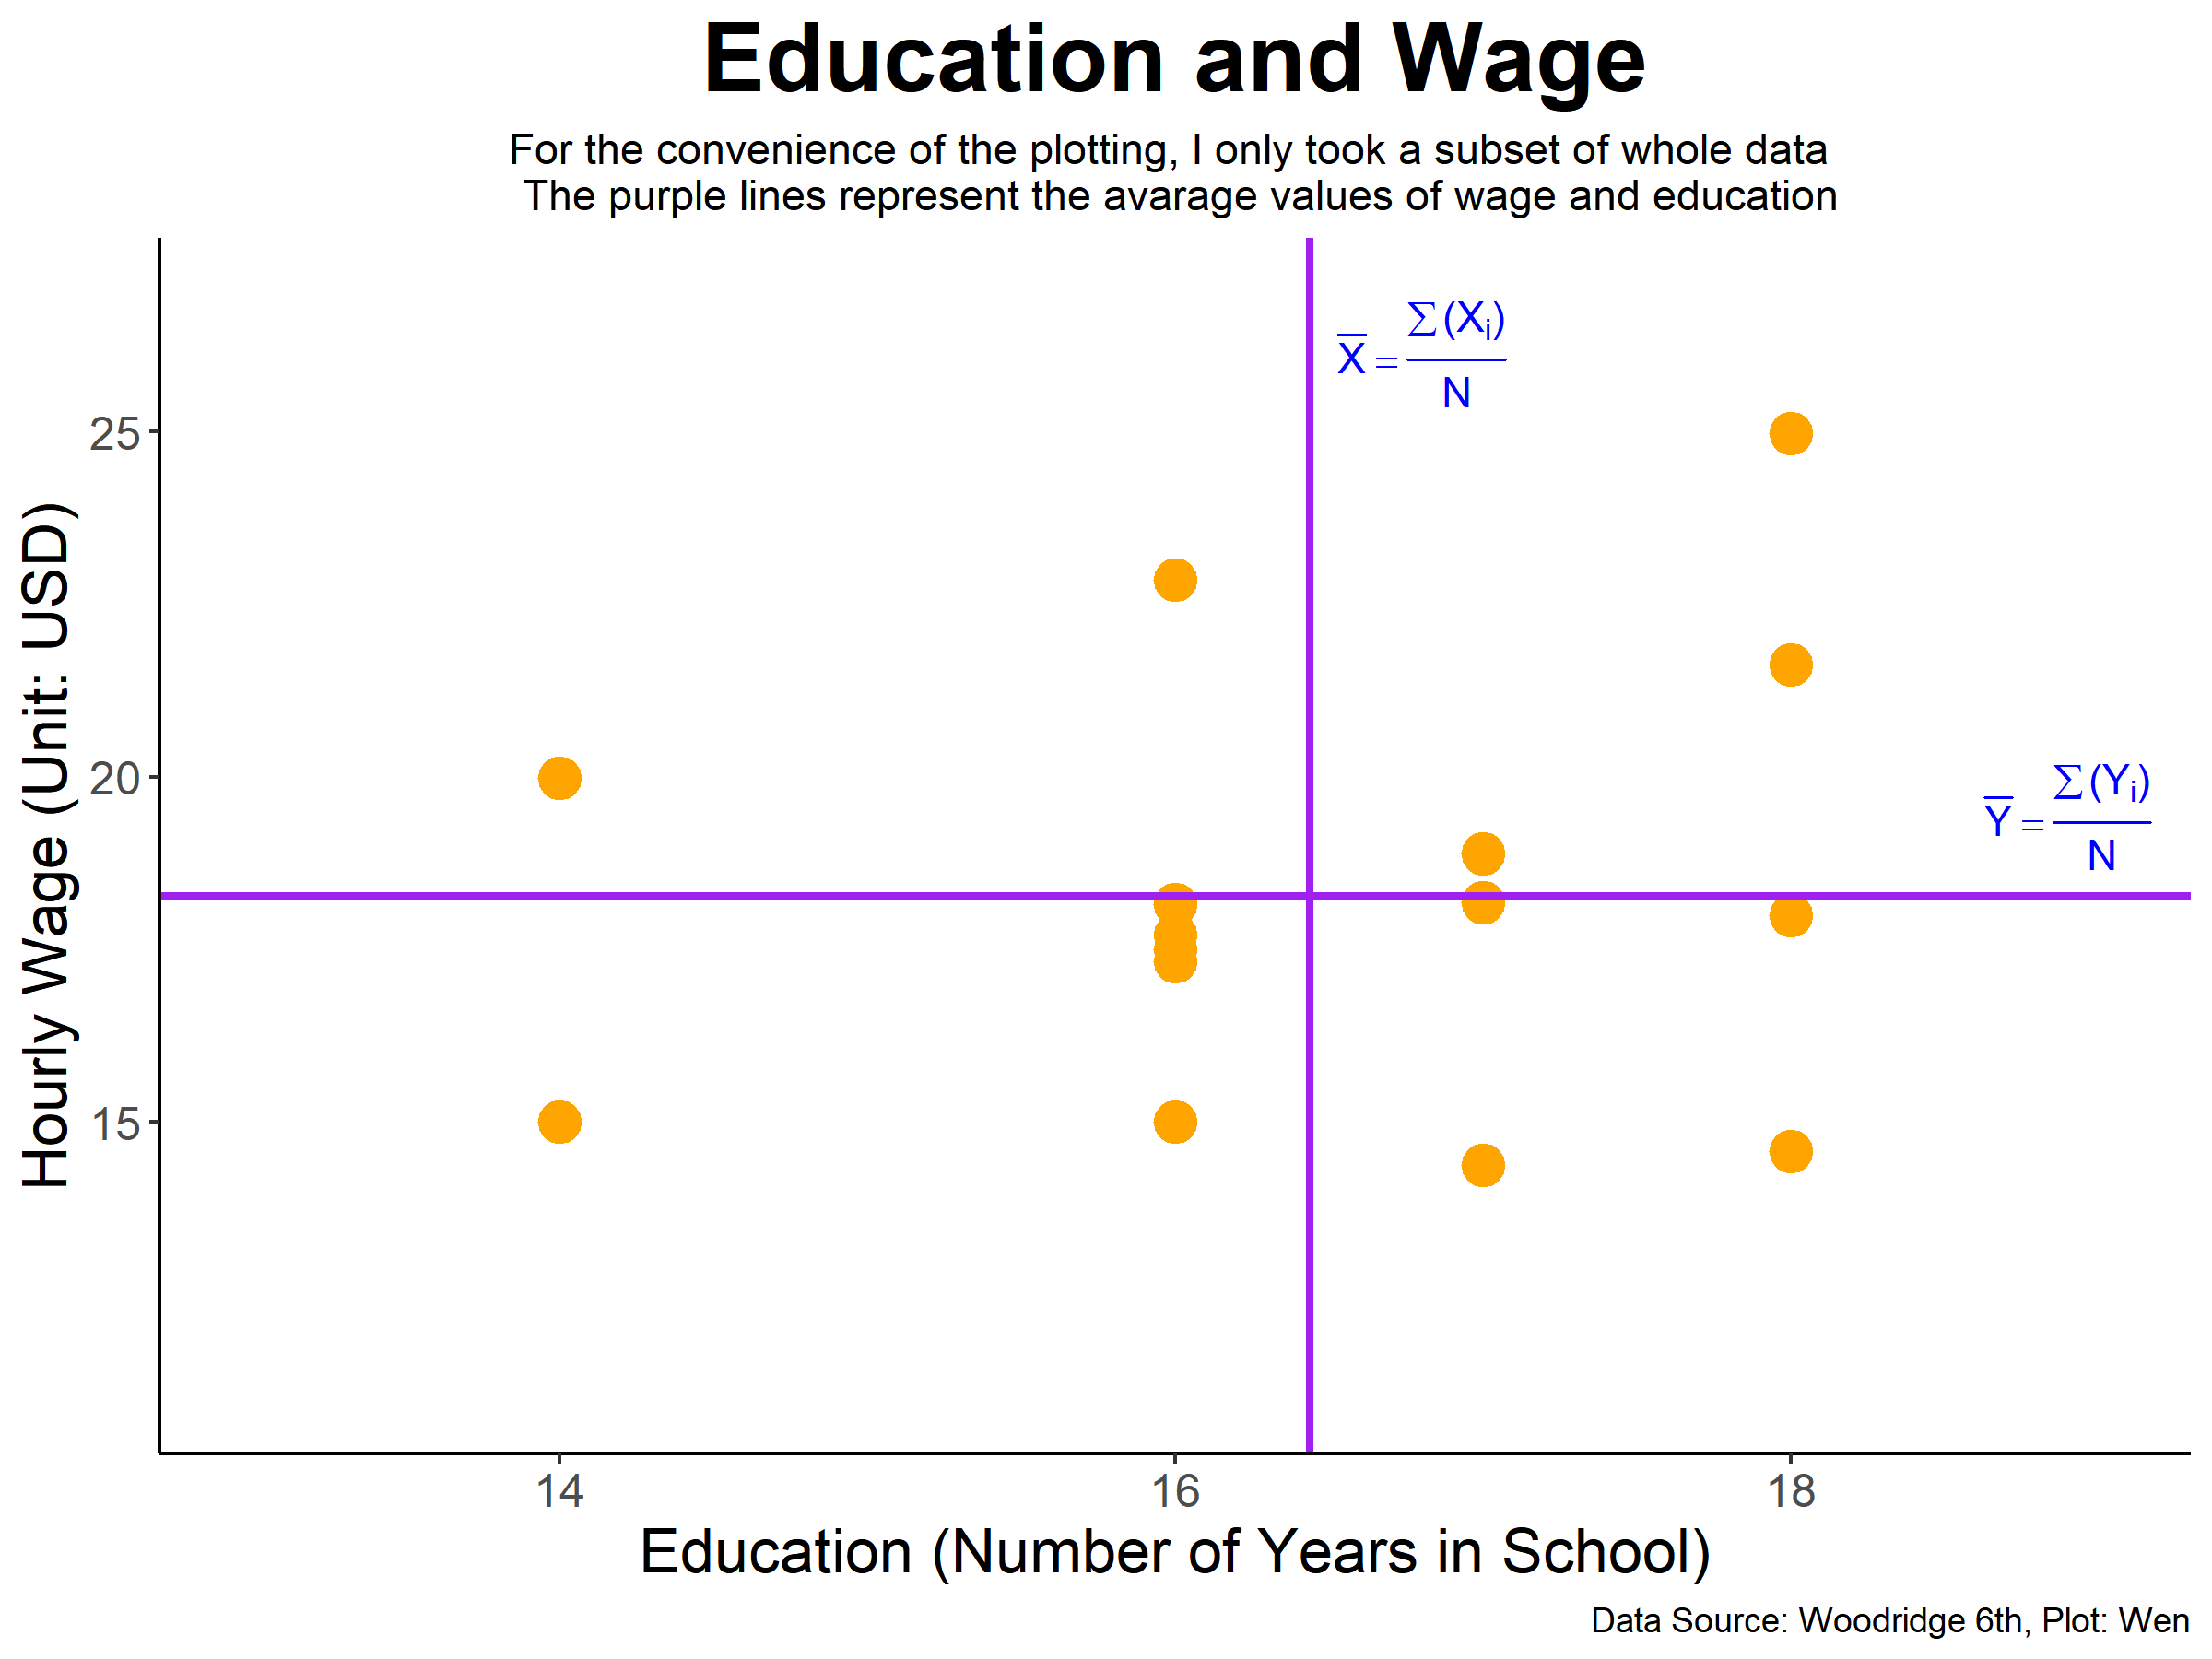
\includegraphics[scale=0.5]{images/plot1.png}
\end{center}

\end{frame}


\begin{frame}{Covariance Visualized (3/3)}
\vspace{0.2 cm}

\begin{center}
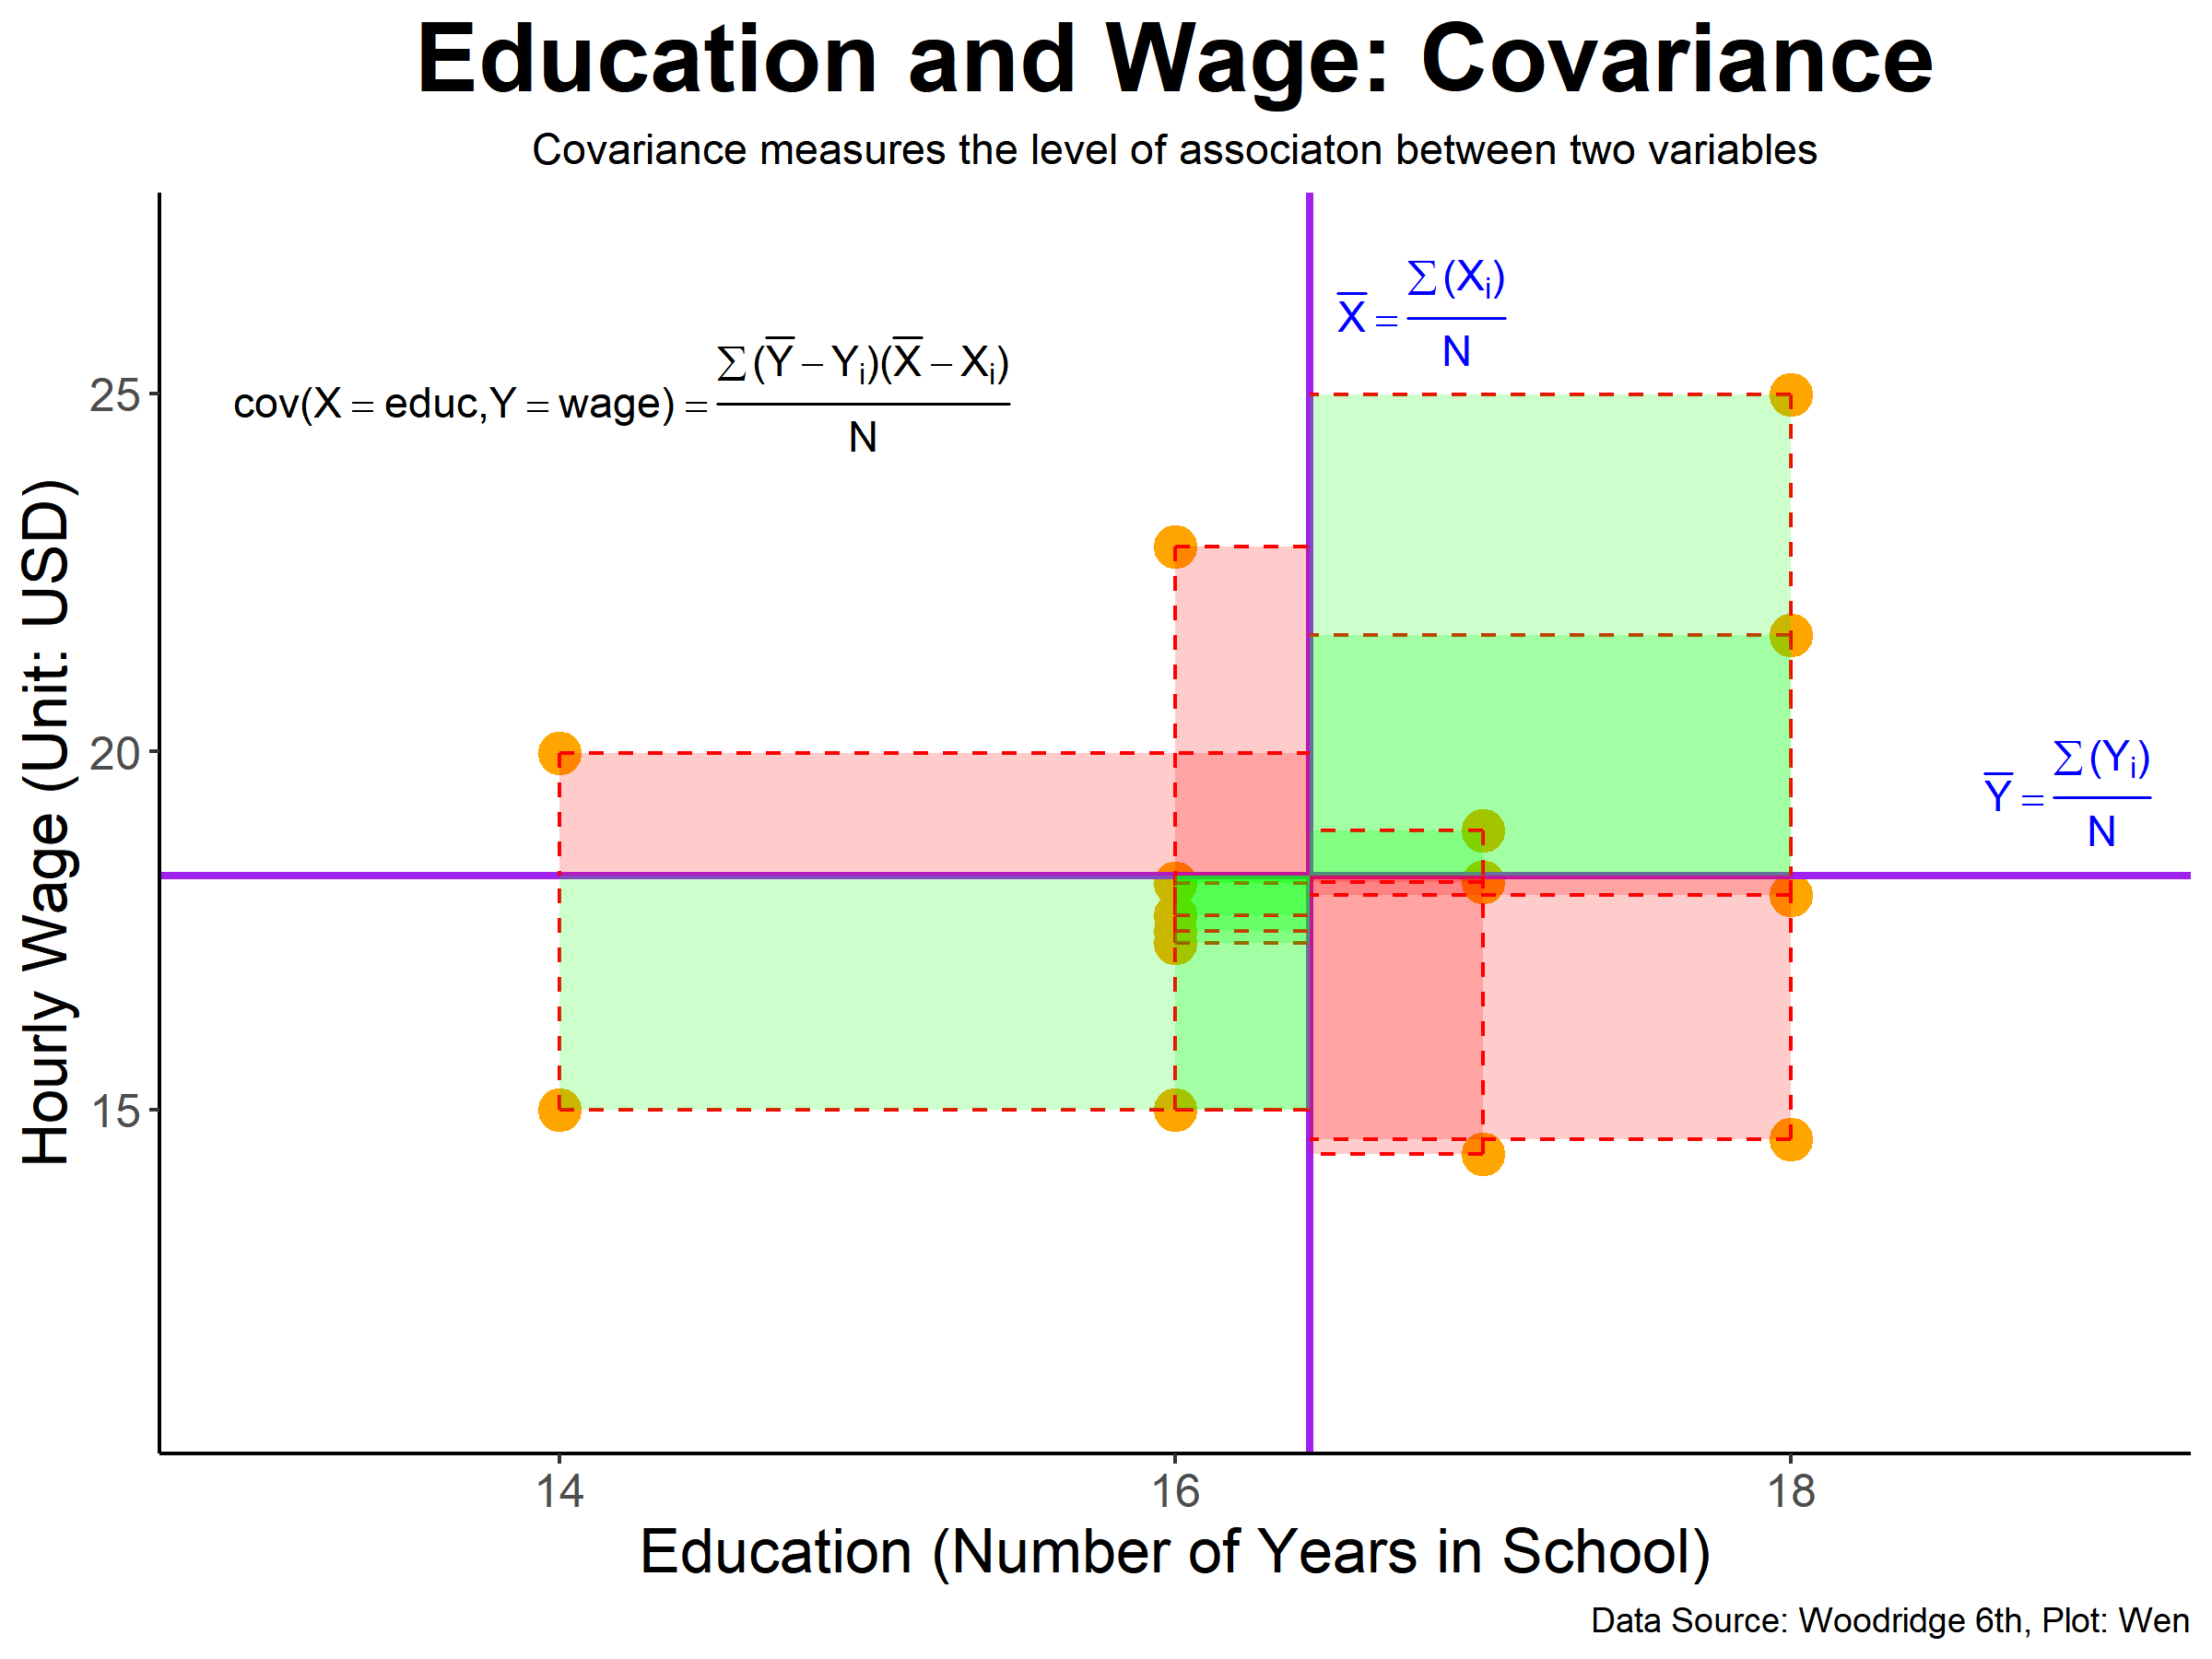
\includegraphics[scale=0.38]{images/plot2.png}
\end{center}

Theoretically, while the green rectangles will have positive dimensions, the red ones will have negative dimensions.

\end{frame}


\begin{frame}{Interpretation of the Covariance}
\begin{itemize}
\item If the total combined area of the green rectangles are larger than that of the red rectangles, two variables can be said \textit{positively} correlated. (Covariance > 0)

\item If the total combined area of the red rectangles are larger than that of the green rectangles, two variables can be said \textit{negatively} correlated. (Covariance < 0)

\item If the total combined area of the rectangles from  each diagonal are equal, then, two variables are said to have no correlation.  (Covariance = 0)


\end{itemize}
\end{frame}


\begin{frame}{A Problem with the Covariance}

\begin{itemize}
\item A larger positive (or negative) value for the covariance indicates a strong positive (or negative) relationship.
\item However, one problem with using covariance as the strength of the relationship is that the value of the covariance depends on the units of measurement for $x$ and $y$. 
\item Consider the following two cases, which will have a higher covariance? 

\end{itemize}


\begin{center}
\begin{tabular}{c|c|c}
\hline 
 & Variable A & Variable B \\ 
\hline 
Case 1 & Height in Feet & Height in Feet \\ 
\hline 
Case 2 & Height in Inch & Height in Inch \\ 
\hline 
\end{tabular}
\end{center}

Therefore, the interpretation of the covariance should be cautious. We can also consider using a standardized measure $\rho$

\end{frame}

\begin{frame}{Correlation Coefficient $\rho$}

\textbf{Correlation Coefficient} (standardized covariance)
$$\rho_{xy} = \frac{\sigma_{xy}}{\sigma_x \sigma_y} \quad\text{or}\quad r_{xy} = \frac{s_{xy}}{s_x s_y}   $$

\begin{flushright}
\textit{Excel Formula: =Correl(var1\_Range, var2\_Range)}
\end{flushright}

\begin{itemize}
\item This measure will be ranging between -1.00 and 1.00.

\end{itemize}


\begin{tabular}{c|c}
\hline 
Size of the Correlation & Interpretation \\ 
\hline 
.90 to 1.00 (-.90 to -1.00) & Very high positive (negative) correlation \\ 
\hline 
.70 to .90 (-.70 to -.90) & High positive (negative) correlation \\ 
\hline 
.50 to .70 (-.50 to -.70) & Moderate positive (negative) correlation \\ 
\hline 
.30 to .50 (-.30 to -.50) & Low positive (negative) correlation \\ 
\hline 
0 to .30 (0 to -.30) & Negligible correlation \\ 
\hline 
\end{tabular} 

 

\end{frame}






\begin{frame}{Check Your Understanding (1/3)}
\vspace{0.2 cm}

\begin{center}

Q: How would you (verbally) describe the level of association between the two variables in each of the following cases?
\vspace{0.5 cm}

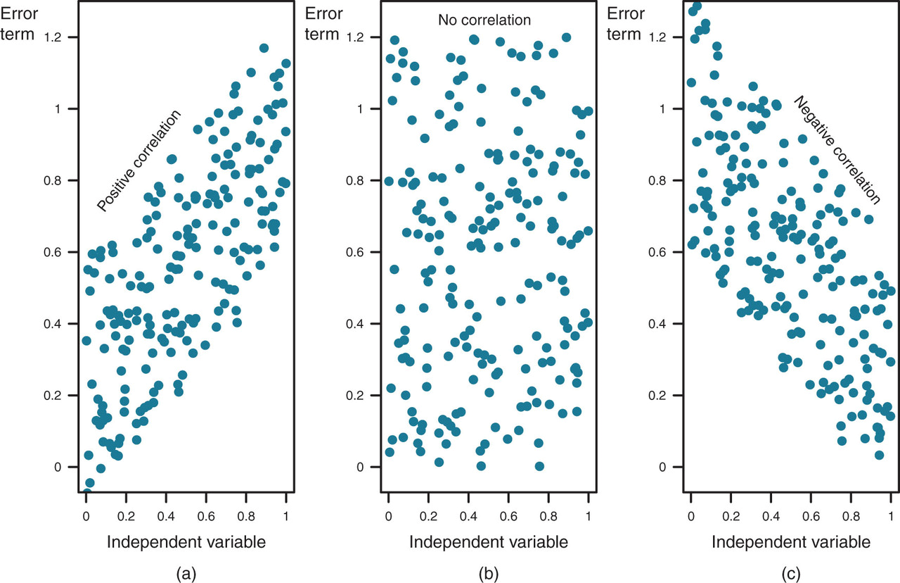
\includegraphics[scale=0.5]{images/correlationsAllSorts.png}
\end{center}

\end{frame}



\begin{frame}{Check Your Understanding (2/3)}

Guessing the correlation coefficient

\begin{itemize}
\item \href{https://www.rossmanchance.com/applets/GuessCorrelation.html}{Click to play this simulation game}
\item \href{https://istics.net/Correlations/}{(Another version)}

\end{itemize}
\end{frame}

\begin{frame}{Check Your Understanding (3/3)}

A measure of linear association between two quantitative variables is the

\begin{itemize}
\item a. variance
\item b. coefficient of variation
\item c. correlation coefficient
\item d. standard deviation

\end{itemize}

\end{frame}

\begin{frame}{Check Points Before Move On}

\begin{itemize}
\item From data to a frequency distribution to a histogram to a fitting line
\item From a frequency distribution to a cumulative relative frequency distribution
\item Mean and median as the measure of the central tendency
\item Variance and standard deviation as the measure of the spread
\item Two areas of assessment in evaluating the linear association between two variables. 
\item Covariance and correlation coefficient as the measure of the linear association between two variables


\end{itemize}


\end{frame}


\subsubsection{Weighted Average}
\begin{frame}{Other Measures of Central Tendency}



\textbf{Weighted Mean}
$$\mu = \frac{\sum_{i=1}^{N}w_ix_i}{\sum_{i=1}^{N}w_i} \quad\text{or}\quad \bar{x} = \frac{\sum_{i=1}^{n}w_ix_i}{\sum_{i=1}^{n}w_i}   $$
\begin{center}
($w_i = \text{the weight of the observation}$ $i$ )\end{center}
In the mathematical mean, the weight of the each item is considered the same as $1/N$. But in the weighted mean the weight is different for each observation. 

\begin{flushright}
\textit{Excel Formula: =SUMPRODUCT($x_i$, $w_i$)/SUM($w_i$)}
\end{flushright}



\textbf{Mode} 
\begin{center}
The most frequent observations
\begin{flushright}
\textit{Excel Formula: =Mode.mult(Range}) or \textit{=Mode.sngl(Range)}

\end{flushright}
\end{center}
\end{frame}


\begin{frame}{Check Your Understanding}

A college sophomore has completed so far 3 courses. He received an A for a 5 credit hour course, a B for a 4 credit hour course, and a C for a 3 credit hour course.  What is his GPA?

\begin{itemize}
\item a.	2.83
\item b.	3.50
\item c.	3.00
\item d.	3.17

\end{itemize}

\vspace{0.5 cm}
Please show the steps in Excel.


\end{frame}


\subsubsection{Coefficient of Variation}
\begin{frame}{Other Measures of Variability using Standard Deviation}
\textbf{Coefficient of Variation} or Relative Standard Deviation
$$ \frac{\sigma}{\mu} \quad\text{or}\quad \frac{s}{\bar{x}} $$

Advantage
\begin{itemize}
\item Understand the variations in relation to the mean.
\item Making the comparison of the variations between variables with different unit and size.
\end{itemize}

Disadvantage
\begin{itemize}
\item Cannot use it when the mean is zero. 
\end{itemize}


\end{frame}



\begin{frame}{Check Your Understanding}
Please compare the level of variations among the following stock price data. (Average stock price observed sequentially.) Explain why the use of coefficient of variation is more useful in this case.


\begin{center}
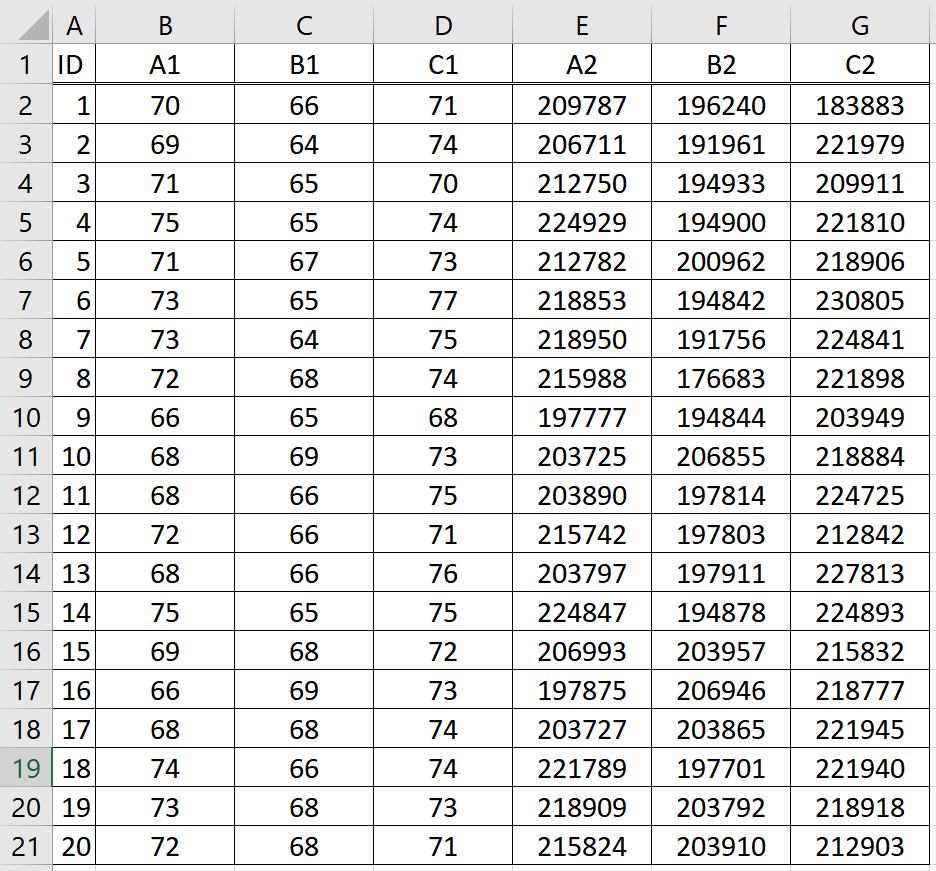
\includegraphics[scale=0.4]{images/ch2StockData.png}

\end{center}
\end{frame}


\subsubsection{Percentiles and Quartiles}
\begin{frame}{The Measures of Location: Percentiles and Quartiles (1/5)}

\begin{center}
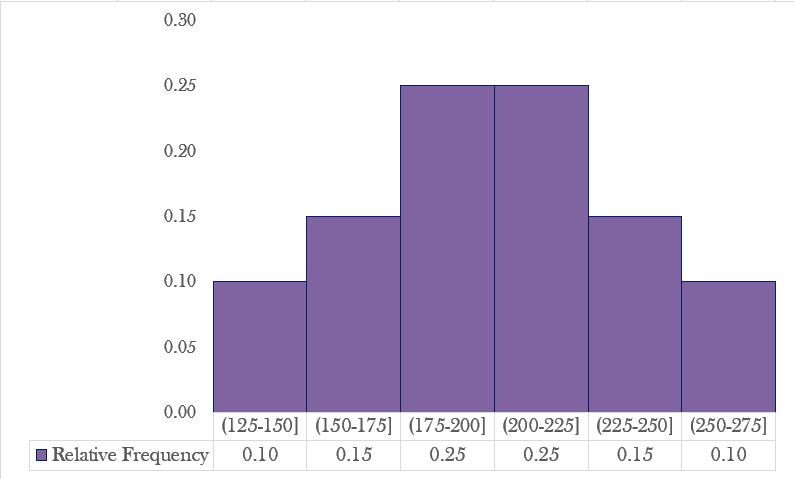
\includegraphics[scale=0.5]{images/ch2PercentilesNaked.png}
\end{center}

\begin{center}
\textit{What do you see and what can you discuss about the data/histogram?
}
\end{center}
\end{frame}

\begin{frame}{The Measures of Location: Percentiles and Quartiles (2/5)}

\begin{center}
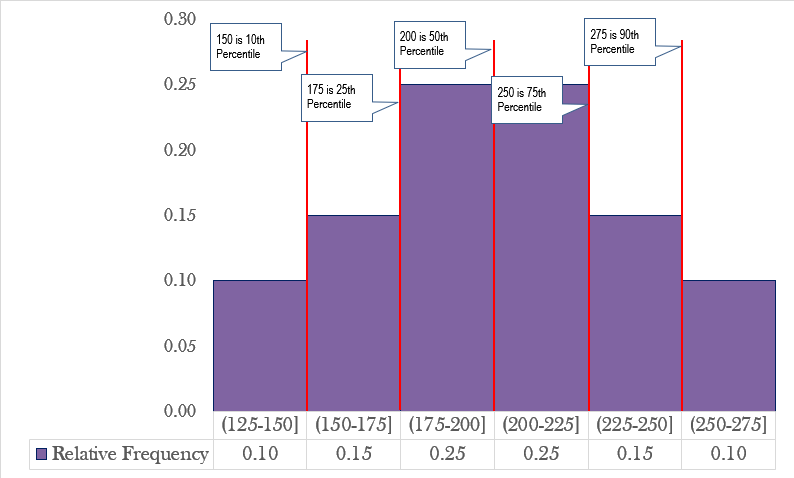
\includegraphics[scale=.5]{images/ch2Percentiles.png}

\end{center}

\end{frame}




\begin{frame}{The Measures of Location: Percentiles and Quartiles (3/5)}

Steps to find a \textbf{Percentile}
\begin{itemize}
\item Step 1: identify the location of the \textit{p}th percentile
$$L_p = \frac{p}{100} (n + 1) $$

\item Step 2: the \textit{p}th percentile can be identified through a series of well defined steps (aka. algorithm) using the $L_p$ identified above. 
\item (I will only ask you to find a percentile using the Excel formula.)
\end{itemize}
\begin{flushright}
\textit{Excel Formula: =Percentile.exc(DataRange, Percentile)
}
\end{flushright}

\end{frame}



\begin{frame}{The Measures of Location: Percentiles and Quartiles (4/5)}

\textbf{Quartiles} divide the entire data into four equal size groups.




\begin{itemize}
\item 25th Percentiles (or $Q_1$ = \textbf{first quartile})
\item 50th Percentiles (or $Q_2$ = \textbf{second quartile}, or the \textbf{median})
\item 75th Percentiles (or $Q_3$ = \textbf{third quartile})
\end{itemize}

\begin{flushright}
\textit{Excel Formula: =Quartile.exc(DataRange, Quart)}

\end{flushright}


(The \textit{quintiles} and the \textit{deciles} are similar concepts.)

\end{frame}


\begin{frame}{The Measures of Location: Percentiles and Quartiles (5/5)}
\begin{center}
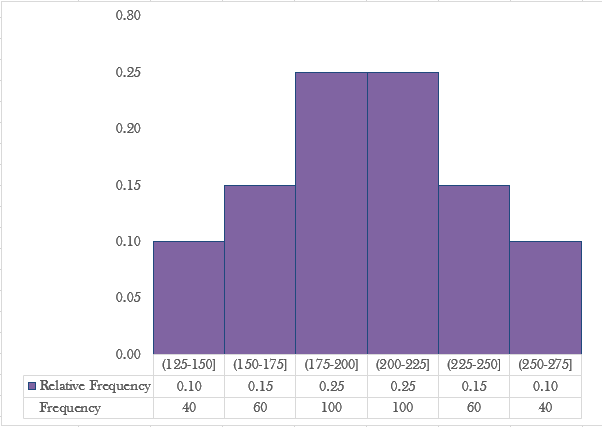
\includegraphics[scale=0.5]{images/ch2Quartiles.png}

\textit{Can you find all three quartiles from this distribution?
}
\end{center}
\end{frame}


\begin{frame}{Check Your Understanding}

A data was collected about starting salaries of all graduates from a small local university who were hired within three months after graduation. The starting salary of John, a graduate from the business college, is at the 77\% percentile in the data. It means that approximately 

\begin{itemize}
\item a.	77\% of the graduates were offered more than John and 23\% less than John
\item b.	77\% of the graduates were offered less than John and 23\% more than John
\item c.	John’s salary is the average of the top 77\% of the starting salaries
\item d.	John’s salary is the average of the bottom 77\% of the starting salaries

\end{itemize}




\end{frame}





\subsubsection{Boxplot}
\begin{frame}{One Important Application of the Quartiles - Boxplot(1/4)}

\textbf{Inter-Quartile Range} (IQR) is an \textit{interval} where the mid 50 percent of the data points are concentrated.

$$IQR = Q_3 - Q_1$$
It excludes the smallest 25\% and largest 25\% of the data. 


\end{frame}


\begin{frame}{Check Your Understanding (1/2)}

The median of a data set is

\begin{itemize}
\item a.	the second quartile
\item b.	the 50th percentile
\item c.	the middle value when the number of values is odd and they are arranged in ascending order
\item d.	the average of the two middle values when the number of values is even and they are arranged in ascending order
\item e.	all the above

\end{itemize}

\end{frame}


\begin{frame}{Check Your Understanding (2/2)}

The interquartile range is used as a measure of variability to overcome what disadvantage of the range?

\begin{itemize}
\item a.	the range is typically too short
\item b.	the range is difficult to compute
\item c.	the range is influenced too much by extreme values
\item d.	the range is never negative
\end{itemize}

\end{frame}



\begin{frame}{One Important Application of the Quartiles - Boxplot(2/4)}

\begin{center}
The Anatomy of a Boxplot
\vspace{0.3cm                                                                                                                                                                                                                               }

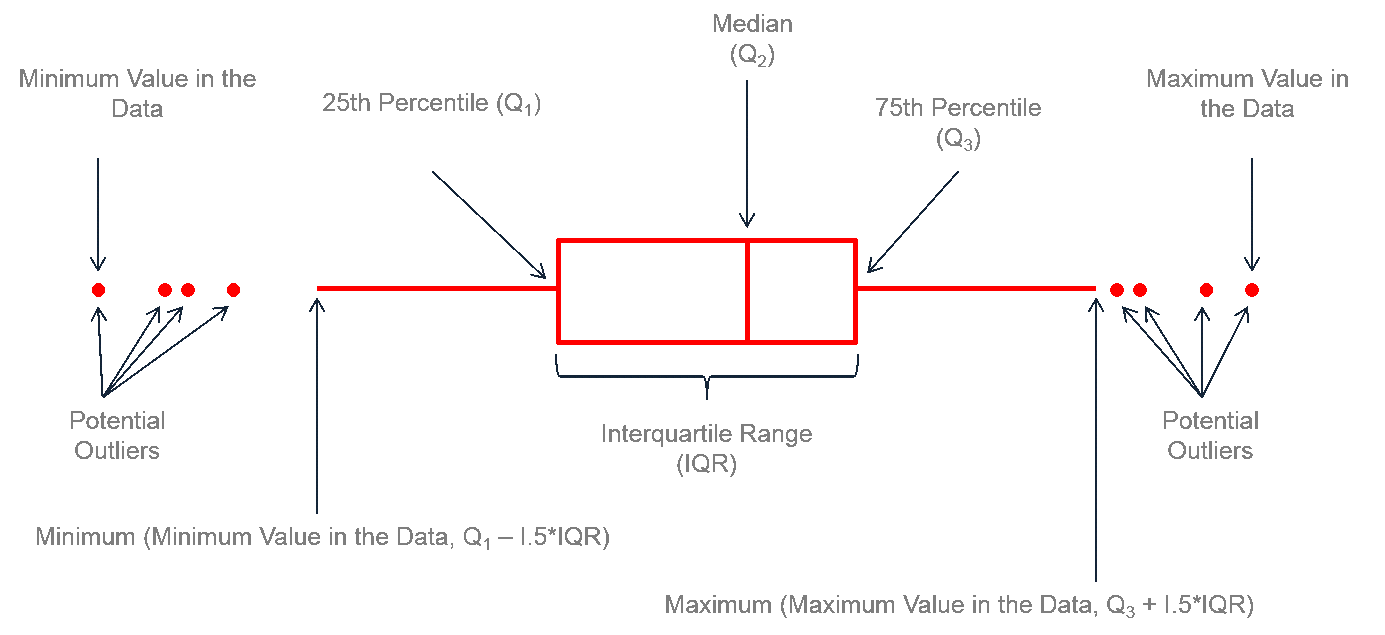
\includegraphics[scale=0.31]{images/ch2BoxPlotAnatomy.png}
\end{center}

\begin{flushright}
\begin{scriptsize}
\textit{Reference: https://www.r-graph-gallery.com/boxplot.html
}\end{scriptsize}
\end{flushright}

\end{frame}

\begin{frame}{One Important Application of the Quartiles - Boxplot(3/4)}

\begin{multicols}{2}

\begin{center}
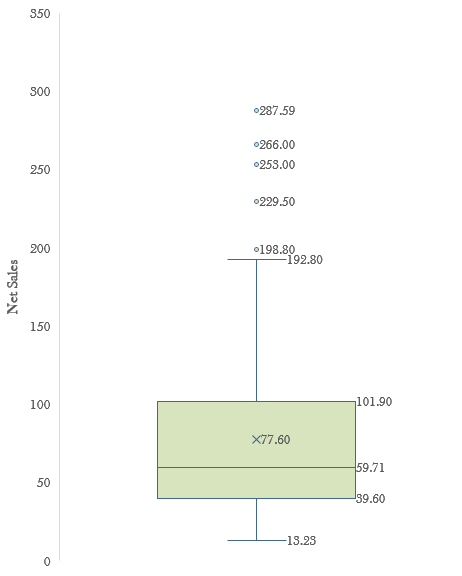
\includegraphics[scale=0.5]{images/ch2BoxPlotSingle.png}
\end{center}


\begin{center}
\vspace{0.3 cm}
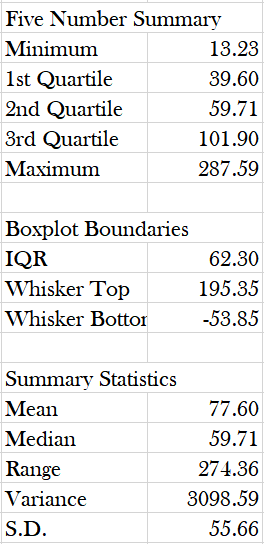
\includegraphics[scale=0.5]{images/ch2BoxPlotSingleNumerics.png}

\end{center}

\end{multicols}
\end{frame}


\begin{frame}{One Important Application of the Quartiles - Boxplot(4/4)}

\begin{center}
Boxplot makes it easier to compare multiple groups
\vspace{0.3cm}

\includegraphics[scale=0.17]{images/ch2BoxPlotGroup.jpg}

\end{center}

\end{frame}


\subsubsection{Z-score and Empirical Rule}
\begin{frame}{The Measures of Location Using Standard Deviation (1/4)}

Standard deviation as the ruler: \textbf{z-score} (standardized of $x_i$)
$$ z_i = \frac{x_i - \mu}{\sigma} \quad\text{or}\quad z_i = \frac{x_i - \bar{x}}{s} $$

\begin{flushright}
\textit{Excel Formula: =Standardize(x, mu, sd)
}
\end{flushright}
For example, in the \textit{net sales} variable, 
\begin{itemize}
\item it has $\bar{x} = 77.60$, $s = 55.66$
\end{itemize}



\begin{center}
\begin{scriptsize}
\begin{tabular}{c|c|c|c}
\hline 
Value of x & Steps to z & z-score & Interpretation \\ 
\hline 
40.78 & (40.78 - 77.60)/55.66 & -.66 & .66 s.d. less than the average. \\ 
\hline 
77.60 & (77.60 - 77.60)/55.66 & .00 & The same with the average \\ 
\hline 
133.26 & (133.26 - 77.60)/55.66 & 1.00 & 1 s.d. larger than the average. \\ 
\hline 
\end{tabular} 
\end{scriptsize}
\end{center}

\end{frame}


\begin{frame}{The Measures of Location Using Standard Deviation (2/4)}

\begin{center}
\includegraphics[scale=0.18]{images/ch2EmpiricalRule.png}
\end{center}

The \textbf{empirical rule} shows the \textit{approximate} fraction of observations concentrated within one, two, and three s.d. from the mean of a normal distribution.

\end{frame}

\begin{frame}{The Measures of Location Using Standard Deviation (3/4)}

Detection of the \textbf{Outliers}

\begin{itemize}
\item Since the empirical rule tells that about 99.7\% of the observations are concentrated within the 3 s.d. distances.
\item Outside of the boundaries, there will be only about 0.3\% observations.
\item Therefore, those fell outside are considered rare occurrences.
\item So they are considered "outliers".
\item Outliers will have $\textsf{z-score} > 3$ or $\textsf{z-score} < -3$. 
\end{itemize}

\end{frame}

\begin{frame}{The Measures of Location Using Standard Deviation (4/4)}

\begin{itemize}
\item This usage of standard deviation, mean, and the distributional characteristics are extremely important.
\item The standardized value of x, or the z-score,  
\begin{itemize}
\item tells whether it is larger than the average
\item tells how common the value is when compared with other observations in the data
\item can be easily related to the percentile. For example,
\begin{itemize}
\item If $\textsf{z-score}=-2$, then the number is likely a 16 percentile. 
\item If $\textsf{z-score}= 2$, then the number is likely a 98 percentile. 
\end{itemize}

\end{itemize}
\end{itemize}

\end{frame}



\begin{frame}{Histogram and the Fit Line (1/2)}


\begin{center}
\includegraphics[scale=0.3]{images/ch2HistogramFitting.png}
\end{center}
The fit line that approximates the histogram is defined as: 
$$ \frac{1}{\sigma\sqrt{2\pi}} e^{-\frac{1}{2} \left(   \frac{x-\mu}{\sigma}\right)^2} $$

\end{frame}

\begin{frame}{Histogram and the Fit Line (2/2)}

The comparisons of Excel solutions on finding the percentile and the fraction

\begin{scriptsize}
\begin{center}
\begin{tabular}{l|c|c}
\hline 
 & Percentile & Fraction before X \\ 
\hline 
Histogram & =Percentile.exc(Range, p) & Many steps... \\ 
\hline 
Fit Line & =Norm.inv(p, mean, sd) & =Norm.dist(x, mean, sd, TRUE) \\ 
\hline 
Fit Line (Z) & =Norm.s.inv(p)  & =Norm.dist(z, TRUE) \\ 
\hline 
\end{tabular} 
\end{center}
\end{scriptsize}


\end{frame}









\section{III. Introduction to Probability}


\begin{frame}{Why We Learn Probability (1/2)}

In many cases, to make a decision, we consider many "variables", or many factors involved in the decision making process.

\begin{itemize}
\item $\textsl{Budget Needed} = \textsl{Planned Spending} - \textsl{Cash at Hand}$
\item $\textsl{Inventory to Prepare} = \textsl{Upcoming Demand} - \textsl{On-hand Inventory}$
\end{itemize}

\vspace{0.3cm}
The quantities such as \textsl{Planned Spending} and \textsl{Upcoming Demand} are considered \textbf{probabilistic}, because we cannot predict those with accuracy. 


\vspace{0.3cm}
The quantities such as \textsl{Cash at Hand} and \textsl{On-hand Inventory} are considered \textbf{deterministic}, because these are quantities we know and/or can exercise control with a great certainties.

\end{frame}



\begin{frame}{Why We Learn Probability (2/2)}

For a probabilistic quantity, if available, we can consider the various possible outcomes with the probabilities associated with each outcome. 


\begin{scriptsize}
\begin{center}

\begin{tabular}{l|c}
\hline
\textbf{Demand} & \textbf{Probability} \\ \hline
25,000          & 10\%                 \\ \hline
26,000          & 15\%                 \\ \hline
27,000          & 25\%                 \\ \hline
28,000          & 25\%                 \\ \hline
29,000          & 15\%                 \\ \hline
30,000          & 10\%                 \\ \hline
\textbf{Total}  & \textbf{100\%}       \\ \hline
\end{tabular}
\end{center}
\end{scriptsize}

A weighted average can help us determine a most likely outcome: 
$$\textsl{Expected Demand} = \sum \textsl{Demand}_i \cdot \textsl{Probability}_i = 27,500$$
In the long run, assuming the probability assigned to each demand scenario does not change, this quantity will be the most likely demand.
\end{frame}


\begin{frame}{Defining Probability}

\begin{block}{Probability Definition}
Probability is the quantitative expression of the chance that an event will occur.
\end{block}

\vspace{0.3cm}
\begin{itemize}
\item The probability of an event A is usually written as $P(A)$ or $Pr(A)$.
\item If $P(A) = 0$, the event has no chance of occurring.
\item If $P(A) = 1$, the event will certainly happen with no doubt.
\item A probability can be obtained through the observation (e.g., past record), logical analysis, and subjective determination.
\end{itemize}

\end{frame}

\begin{frame}{More on Probability}
The probability of an outcome is interpreted as the long-run proportion of the time that the outcome would occur, if the experiment were repeated indefinitely. That is, probability is \textbf{long-term relative frequency}. \footnote{citing from: http://www.math.wsu.edu/faculty/djohnson/}

\begin{center}
\includegraphics[scale=.25]{images/ch3CoinToss.png}

\end{center}


\end{frame}

\subsubsection{Experiment, sample point, sample space, and event}
\begin{frame}{Experiments and Sample Point}

\begin{itemize}
\item An \textbf{experiment} is a process that generates well-defined outcomes. For examples,

\item An experiment outcome is called a \textbf{sample point}.

\end{itemize}

\begin{center}
\begin{tabular}{l|l}
\hline
Experiment        & All Sample Points        \\ \hline
Toss a coin       & Head, tail               \\ \hline
Inspection a part & Defective, non-defective \\ \hline
Roll a die        & 1, 2, 3, 4, 5, 6         \\ \hline
Class Attendance  & 0, 1, 2, 3, ... Max      \\ \hline
\end{tabular}
\end{center}

\end{frame}

\begin{frame}{Sample Space as a Set}

An exhaustive set of sample points of an experiment is called a \textbf{sample space}. Therefore, a sample space is all possible experimental outcomes.

$$ \textsl{Payment method} = \lbrace Amex, Discover, Visa, Master, Others \rbrace$$
$$\textsl{Type of customer} = \lbrace Regular, Promotional \rbrace $$
$$ \textsl{Number of family members} = \lbrace 1, 2, 3, 4, 5, 6, 7, 8, \textsl{above 8} \rbrace$$



\end{frame}







\begin{frame}{Assigning Probabilities}

The probability assigned to each experiment outcome must be between 0 and 1
$$ 0 \leq P(E_i) \leq 1 \text{ for all } i $$

\vspace{0.4 cm}
The sum of the probability for all the sample point must equal to 1
$$ \sum_{i=1}^n P(E_i) = 1 $$

\vspace{0.4 cm}
\textit{This is the same with the relative frequency distribution...
}\end{frame}


\begin{frame}{Assigning Probabilities Using Relative Frequency}

The relative frequency information can be utilized as the basis of the probability. For example,
\vspace{0.3cm}

\begin{center}
\includegraphics[scale=0.4]{images/ch3RelativeFrequency.png}

\vspace{0.3 cm}

\textit{What is the probability of someone who will use a non-proprietary card for shopping? Please use the notation to show the steps.
}
\end{center}

\end{frame}


\begin{frame}{Check Your Understanding}

Consider the experiment of selecting a playing card from a deck of 52 playing cards. Each card corresponds to a sample point with a 1/52 probability.

\begin{itemize}
\item List the sample points in the event an ace is selected.
\item List the sample points in the event a club is selected.
\item List the sample points in the event a face card (jack, queen, or king) is selected.
\item Find the probabilities associated with each of the events in above three questions.
\end{itemize}



\end{frame}




\begin{frame}{Events and Their Probabilities}

An \textbf{event} is a collection of sample points (or experiment outcome).

\vspace{0.3 cm}

The \textbf{probability of an event} is the sum of the probability of the sample points in the event.

\vspace{0.3 cm}

For example, for a six-dimensional dice, the sample space is:
$$\textsl{Roll a dice} = \lbrace 1, 2, 3, 4, 5, 6 \rbrace$$
Each sample outcome has the probability of 1/6. Then, the probabilities for the following events are:

$$ \textsl{P(Results are even)} = P(\lbrace 2, 4, 6 \rbrace) = \frac{1}{6} + \frac{1}{6} + \frac{1}{6} = \frac{1}{2}   $$
$$ \textsl{P(Results are odd)} = P(\lbrace 1, 3, 5 \rbrace) = \frac{1}{6} + \frac{1}{6} + \frac{1}{6} = \frac{1}{2}  $$


\end{frame}

\begin{frame}{Multiphase or Multistage Experiment (1/4)}
Sometimes an experiment is more complicated as it can involve multiple steps, multiple phases, or multiple con-current activities.

$$\textsl{Rolling two dices} = \lbrace (1, 1), (1, 2), (1, 3) ... (6, 6) \rbrace $$
$$\textsl{Completion time of a two-phase project} = \lbrace (2, 7), (2, 8), (3, 7), ... (4, 8) \rbrace $$
$$\textsl{Color combination of two poker cards} = \lbrace (R, B), (R, R), (B, R), (B, B) \rbrace $$

\end{frame}



\begin{frame}{Multiphase or Multistage Experiment (2/4)}

\includegraphics[scale=0.4]{images/ch3MultiPhaseProject.png}

\end{frame}



\begin{frame}{Multiphase or Multistage Experiment (3/4)}

\includegraphics[scale=0.4]{images/ch3MultiPhaseProject2.png}

\end{frame}



\begin{frame}{Multiphase or Multistage Experiment (4/4)}

\includegraphics[scale=0.4]{images/ch3MultiPhaseProject3.png}

Can you find out the followings? 
$$ P(\textsl{Take less than 10 month}) = ?  $$
$$ P(\textsl{Take more than 10 month}) = ?  $$

\end{frame}

\begin{frame}
\begin{center}
\includegraphics[scale=0.26]{images/comfortZone.jpg}

\end{center}
\end{frame}

\subsubsection{Complement Events}

\begin{frame}{Complement of an Event (Or Collectively Exhaustive Events)}

Given an event A, the \textbf{complement} of A is defined to be the event consisting of all sample points that \textit{are not} in A. Therefore, 

$$ P(A) + P(A^c) = 1$$ 
or
$$ P(A) = 1 - P(A^c)$$

\vspace{0.3 cm}

\includegraphics[scale=0.4]{images/ch3VennComplement.png}

\end{frame}

\subsubsection{Addition Law}
\begin{frame}{Addition Law - Union of Multiple Events}

The \textbf{union} of A and B is the event containing all sample points belonging to A or B or both. Therefore, to add both, 

$$ P(A \cup B) = P(A) + P(B) - P(A \cap B)$$ 

\includegraphics[scale=0.4]{images/ch3UnionEvents.png}


\end{frame}


\begin{frame}{Intersection of Multiple Events}

Given two events A and B, the \textbf{intersection} of A and B is the event containing the sample points belonging to both A and B.
\vspace{0.3 cm}
\linebreak It is denoted as $P(A \cap B)$ 

\vspace{0.6 cm}
\includegraphics[scale=0.4]{images/ch3IntersectionEvents.png}

\end{frame}



\begin{frame}{Addition Law for Mutually Exclusive Events}

Two events are said to be \textbf{mutually exclusive} if the events have no sample points in common. or $P(A \cap B) = 0$ 

\vspace{0.4 cm}

\includegraphics[scale=0.4]{images/ch3MutuallyExclusiveEvents.png}

\vspace{0.3 cm}
Therefore, the addition for mutually exclusive events are: 
$$ P(A \cup B) = P(A) + P(B)$$ 

\end{frame}


\begin{frame}{Check Your Understanding (1/2)}

The U.S. Census Bureau provides data on the number of young adults, ages 18–24, who are living in their parents’ home. Let
\vspace{0.3 cm}
\linebreak
M = the event a male young adult is living in his parents’ home
\linebreak
F = the event a female young adult is living in her parents’ home
\vspace{0.3 cm}

If we randomly select a male young adult and a female young adult, the Census Bureau data enable us to conclude P(M)=.56 and P(F)=.42 (The World Almanac, 2006). The
probability that both are living in their parents’ home is .24

\begin{itemize}
\item  What is the probability at least one of the two young adults selected is living in his or her parents’ home?
\item What is the probability both young adults selected are living on their own (neither is living in their parents’ home)?
\end{itemize}

\end{frame}



\begin{frame}{Check Your Understanding (2/2)}

Please see the following exhibit: 

\begin{center}
Promotion Status of Police Officers
\vspace{0.2 cm}

\begin{tabular}{l|c|c|c}
\hline 
 & Men & Women & Total \\ 
\hline 
Promoted & 288 & 36 & 324 \\ 
\hline 
Not Promoted & 672 & 204 & 876 \\ 
\hline 
Total & 960 & 240 & 1,200 \\ 
\hline 
\end{tabular}
\end{center}

Please answer the following questions: 
\begin{itemize}
\item Please identify at least two pairs of collectively exhaustive events.
\item Find the probability of a policeman, regardless of the gender, got the promotion. 
\item Find the intersection event of women and promoted. Also calculate the probability.
\item How to calculate the probability of someone gets promoted given this person is a men? 
\end{itemize}

\end{frame}


\subsubsection{Marginal, Joint, and Conditional Probability}
\begin{frame}{Marginal and Joint Probability}

\begin{center}
Illustration: Promotion Status of Police Officers
\end{center}

\begin{multicols}{2}

\begin{small}
\begin{center}
\begin{tabular}{l|c|c|c}
\hline 
Promoted & M & F & Total \\ 
\hline 
Yes & 288 & 36 & 324 \\ 
\hline 
No & 672 & 204 & 876 \\ 
\hline 
Total & 960 & 240 & 1,200 \\ 
\hline 
\end{tabular}
\end{center}



\begin{center}

\begin{tabular}{l|c|c|c}
\hline 
Promoted & M & F & Total \\ 
\hline 
Yes & .24 & .03 & .27 \\ 
\hline 
No & .56 & .17 & .73 \\ 
\hline 
Total & .80 & .20 & 1.00 \\ 
\hline 
\end{tabular}
\end{center}
\end{small}
\end{multicols}

\textbf{Marginal Probability} is the probability of the event itself. For example, 
$$P(Yes) = .27 \quad\text{or}\quad P(No) = .73$$
$$P(M) = .80 \quad\text{or}\quad P(F) = .20$$


\textbf{Joint Probability} is the probability of the intersection of the two events. For example, 
$$ P(Yes \cap M) = \frac{288}{1200} = .24 \quad\text{or}\quad P(No \cap F) = \frac{204}{1200} = .17 $$
$$ $$


\end{frame}


\begin{frame}{Conditional Probability (1/5)}
\textbf{Conditional Probability} is the probability of an event occurring given that another event has occurred. 

\begin{itemize}
\item Conceptually, the conditional probability is limited or  conditioned by the probability of the precursor event. 
\item For example, the figure below shows the conditional probability as the A within B. The probability of B determines the conditional probability.

\end{itemize}

\begin{center}
\includegraphics[scale=0.3]{images/ch3ConditionalProbability.png}
\end{center}
$$ P(A|B) = \frac{P(A \cap B)}{P(B)} \quad \text{or} \quad P(B|A) = \frac{P(A \cap B)}{P(A)}$$ 

\end{frame}



\begin{frame}{Conditional Probability (2/5)}

\begin{center}
Illustration: Promotion Status of Police Officers
\end{center}

\begin{multicols}{2}

\begin{small}
\begin{center}
\begin{tabular}{l|c|c|c}
\hline 
Promoted & M & F & Total \\ 
\hline 
Yes & 288 & 36 & 324 \\ 
\hline 
No & 672 & 204 & 876 \\ 
\hline 
Total & 960 & 240 & 1,200 \\ 
\hline 
\end{tabular}
\end{center}

\begin{center}
\begin{tabular}{l|c|c|c}
\hline 
Promoted & M & F & Total \\ 
\hline 
Yes & .24 & .03 & .27 \\ 
\hline 
No & .56 & .17 & .73 \\ 
\hline 
Total & .80 & .20 & 1.00 \\ 
\hline 
\end{tabular}
\end{center}
\end{small}
\end{multicols}

The probability of a promotion given the gender is male.

$$P(Yes|M) = \frac{P(Yes \cap M)}{P(M)} = \frac{288}{\textbf{960}} = \frac{.24}{.80} = .30$$

Not to be confused with the probability of a promotion and the male.
$$ P(Yes \cap M) = \frac{288}{\textbf{1200}} = .24 $$

\end{frame}

\begin{frame}{Conditional Probability (3/5)}
\begin{small}

\begin{center}
Illustration: Promotion Status of Police Officers
\end{center}

\begin{multicols}{2}

\begin{small}
\begin{center}
\begin{tabular}{l|c|c|c}
\hline 
Promoted & M & F & Total \\ 
\hline 
Yes & 288 & 36 & 324 \\ 
\hline 
No & 672 & 204 & 876 \\ 
\hline 
Total & 960 & 240 & 1,200 \\ 
\hline 
\end{tabular}
\end{center}

\begin{center}
\begin{tabular}{l|c|c|c}
\hline 
Promoted & M & F & Total \\ 
\hline 
Yes & .24 & .03 & .27 \\ 
\hline 
No & .56 & .17 & .73 \\ 
\hline 
Total & .80 & .20 & 1.00 \\ 
\hline 
\end{tabular}
\end{center}
\end{small}
\end{multicols}

When compare the probability in connection with the gender, we found the followings:

\vspace{0.3 cm} 


The promotion chance for \textbf{male} officers
$$P(Yes|M) = \frac{P(Yes \cap M)}{P(M)} = \frac{288}{960} = \frac{.24}{.80} = .30$$

The promotion chance for \textbf{female} officers
$$P(Yes|F) = \frac{P(Yes \cap F)}{P(F)} = \frac{36}{240} = \frac{.03}{.20} = .15$$


The conclusion: A person's gender limits the promotion probability in this particular example.
\end{small}
\end{frame}


\begin{frame}{Conditional Probability (4/5) - Check Your Understanding}

Please find out all the marginal and joint probabilities. And fill in the results on the table with the blanks.


\begin{center}
Illustration: Promotion Status of Police Officers (Branch K)
\end{center}

\begin{multicols}{2}

\begin{small}
\begin{center}
\begin{tabular}{l|c|c|c}
\hline 
Promoted & M & F & Total \\ 
\hline 
Yes & 125 & 25 & 150 \\ 
\hline 
No & 780 & 156 & 936 \\ 
\hline 
Total & 905 & 181 & 1,086 \\ 
\hline 
\end{tabular}
\end{center}

\begin{center}
\begin{tabular}{l|c|c|c}
\hline 
Promoted & M & F & Total \\ 
\hline 
Yes &  &  &  \\ 
\hline 
No &  & &  \\ 
\hline 
Total &  &  & 1.00 \\ 
\hline 
\end{tabular}
\end{center}
\end{small}
\end{multicols}

\begin{itemize}
\item Please evaluate the conditional probability on the chance of the promotion given someone's gender. What is $P(Yes | M) $ and $ P(Yes | F) $ respectively?
\item What would you comment on the gender equality in the promotion in this particular branch? 
\end{itemize}

\end{frame}


\begin{frame}{Conditional Probability (5/5) - Check Your Understanding}

Let's also review the following case. Please compare the $P(Ace)$ with $P(Ace | Club).$

\begin{center}
Illustration: Poker Cards (Jokers Excluded)
\end{center}

\begin{center}
\begin{tabular}{l|c|c|c}
\hline 
& $ \text{Club} $ & $\text{Club}^C$ & Total \\ 
\hline 
$\text{Ace} $ & 1 & 3 & 4 \\ 
\hline 
$\text{Ace}^C $ & 12 & 36 & 48 \\ 
\hline 
Total & 13 & 39 & 52 \\ 
\hline 
\end{tabular}
\end{center}

\begin{itemize}
\item What can you comment about the probability of picking an ace from a deck of cards and that of picking an ace from the club? 

\item Does the choice of the flower interfere with the chance of picking an ace? 
\end{itemize}

\end{frame}


\subsubsection{Independence}
\begin{frame}{Independent Events}

When the followings are true, then we call A and B are independent events. That is, neither has influence over the chance of the other.

$$P(A|B) = P(A)$$
$$P(B|A) = P(B)$$

Q: If A and B are independent events and $P(A|B) = P(A)$, is this always true? $P(B|A) = P(B)$

\end{frame}

\subsubsection{Multiplication Law}
\begin{frame}{Multiplication Law}

The multiplication law says the following: 

$$P(A \cap B) = P(B)P(A|B)$$
$$P(A \cap B) = P(A)P(B|A)$$

\begin{small}
Remember this? Instead of trying to memorize the law, transform it from the conditional probability.
\end{small}

$$P(A|B) = \frac{P(A\cap B)}{P(B)} $$

For independent events, the multiplication law is simply
$$P(A \cap B) = P(A)P(B) $$ 
(Because $P(A|B) = P(A)$ or $P(B|A) = P(B)$ )

\end{frame}


\begin{frame}{Check Your Understanding}

An experiment A has two mutually exclusive sample points. Let's call these $A_1$ and $A_2$. The conditional probability of $B$ given each of the $A$'s sample points are known as below. Please complete the rest of the table. 


% Please add the following required packages to your document preamble:
% \usepackage{graphicx}
\begin{table}[]
\resizebox{\textwidth}{!}{%
\begin{tabular}{c|c|c|c|c}
\hline
\textbf{Events} & \textbf{Marginal} & \textbf{Conditional} & \textbf{Joint}     & \textbf{Updated} \\ \hline
$A_1$           & $P(A_1) = .65$    & $P(B|A_1) = .02$     & $P(A_1\cap B) = ?$ & $P(A_1|B) = ?$   \\ \hline
$A_2$           & $P(A_2) = ?$      & $P(B|A_2) = .05$     & $P(A_2\cap B) = ?$ & $P(A_2|B) = ?$   \\ \hline
                & 1.00              &                      & $P(B) = ?$         &                  \\ \hline
\end{tabular}%
}
\end{table}
\begin{flushright}
\begin{scriptsize}
(Note: The original marginal probability is updated based on the newly obtained evidences provided through the conditional probability. This is a simple example of the Bayes Theorem.) 
\end{scriptsize}
\end{flushright}



\end{frame}

\subsubsection{Graphical Tools and More}

\begin{frame}{Bonus - Graphical Tools to visualize the Probability (1/2)}

\begin{center}
Addition law visualization - \textbf{Venn's Diagram}

\vspace{0.3 cm}

\includegraphics[scale=0.3]{images/ch3VennComplement.png}

\vspace{0.3 cm}

Joint probability visualization - \textbf{Matrix Table} (or Cross Tabulation)

\vspace{0.3 cm}
\begin{tabular}{l|c|c|c}
\hline 
Promoted & M & F & Total \\ 
\hline 
Yes & .24 & .03 & .27 \\ 
\hline 
No & .56 & .17 & .73 \\ 
\hline 
Total & .80 & .20 & 1.00 \\ 
\hline 
\end{tabular}
\end{center}


\end{frame}

\begin{frame}{Bonus - Graphical Tools to visualize the Probability (2/2)}

\begin{center}

Multiplication law visualization - \textbf{Tree Diagram}

\vspace{0.3 cm}

\includegraphics[scale=0.30]{images/ch3TreeDiagram.png}

\end{center}

\end{frame}

\begin{frame}{Bonus: Saliva Based COVID19 Testing - A Bayesian Framework}


\begin{flushleft}
\includegraphics[scale=0.255]{images/ch3SalivaBayesian.png}

\end{flushleft}
\end{frame}



\section{IV. Probability Distributions}



\subsection{Overview}
\begin{frame}
\subsectionpage
\end{frame}


\begin{frame}{Overview: What We Know about Probability So Far}

What we have learned in the previous section - Probability:
\begin{itemize}
\item An event can be deterministic or probabilistic;
\item When the uncertainties are involved, by assigning probability to a specific outcome, we allow the solutions to be more inclusive;
\item The term fraction, proportion, relative frequency, and probability are interchangeable;
\item When a probability is assigned to all experimental outcomes, it forms a probability distribution. 
\end{itemize}
\end{frame}

\begin{frame}{Experimental Outcomes and Random Variable}

We use the term \textbf{random variable} to numerically describe the sample outcomes.
\begin{itemize}
\item A variable can be understood as a container that can store values;
\item The name \textit{random variable} implies that we can store any values in the variable.
\item The type of the variable can limit the way the experimental outcomes are being described.
\end{itemize}

\begin{center}
\includegraphics[scale=0.4]{images/section4VariableValue.jpg}

\end{center}

\end{frame}


\begin{frame}{Check Your Understanding}

Consider the experiment of tossing a coin twice. 
\begin{itemize}
\item List the experimental outcomes;
\item Define a random variable $x$ that represents the number of heads occurring on the two tosses;
\item Show what value the random variable $x$ would assume for each of the experimental outcomes. 
\end{itemize}

\end{frame}

\begin{frame}{Discrete Random Variable}
A \textbf{discrete random variable} assumes either a finite number of values or an infinite sequence of values. For example, 

\begin{center}
\includegraphics[scale=0.4]{images/section4DiscreteRandomExample.png}
\end{center}

The probability of a specific outcome can be obtained and it is meaningful. 

\end{frame}



\begin{frame}{Continuous Random Variable}
A \textbf{continuous random variable} assumes any numerical value in an interval or collection of intervals. For example, 
\begin{center}
\includegraphics[scale=0.4]{images/section4ContinuousRandomExample.png}
\end{center}

The probability of a specific outcome cannot be obtained and it is meaningless. We are interested in the probability of a section. 

\end{frame}


\begin{frame}{Check Your Understanding}

Here is a list of experiments. Please make up your own random variable and discuss whether the variable is discrete or continuous. 

\begin{itemize}
\item Take a 20-question examination
\item Observe cars arriving at a tollbooth for 1 hour
\item Audit 50 tax returns
\item Observe an employee's phone calls to potential buyers
\item Weight a shipment of goods
\end{itemize}

\end{frame}


\subsection{Discrete Probability Distributions}

\begin{frame}
\subsectionpage
\end{frame}


\begin{frame}{Components of a Discrete Probability Distribution}

See below for a typical discrete probability distribution: 


\begin{center}
Prob. Dist. for Number of Broken Parts on a Five-Part Machine

\vspace{0.2 cm}
\begin{tabular}{l|r} 
\hline
$x$ & $f(x)$  \\ 
\hline
\hline
0     & .5905     \\ 
\hline
1     & .3281     \\ 
\hline
2     & .0729     \\ 
\hline
3     & .0081     \\ 
\hline
4     & .0005     \\ 
\hline
5     & 1.0E-5    \\
\hline
\end{tabular}
\end{center}

\begin{itemize}
\item The \textbf{first column} is all the possible values of $x$. The $x$ also represents the all the possible outcomes of the experiment. 
\item Instead of using $P(x)$, the \textbf{second column} uses $f(x)$, implies the probability is some function of the $x$. 
\end{itemize}


\end{frame}

\begin{frame}{Visualization of a Discrete Probability Distribution}

\begin{center}
\includegraphics[scale=0.3]{images/section4DevelopingDiscreteProbDist.png}
\end{center}

\begin{center}
We have seen similar graphs in the past. Also, 

$$f(x_i) \geq 0$$
$$\sum_{i=0}^{N=5} f(x_i) = 1 $$


\end{center}
\end{frame}


\subsubsection{Empirical Discrete Distribution Definition}
\begin{frame}{Empirical Discrete Distribution}


Please note that $x$ here is NOT a nominal scale measure. It implies the value of $x$ can become the basis of calculations.

\vspace{0.3 cm}
When a relative frequency distribution is used to obtain the values of $f(x)$, we call such probability distribution as \textbf{empirical discrete distribution}.

\vspace{0.3 cm}

The term \textbf{empirical} means "\textit{based on, concerned with, or verifiable by observation or experience rather than theory or pure logic}."


\vspace{0.3 cm}
In this case, we map $x$ with $f(x)$ using the past records. That is, \textbf{$x$ $\rightarrow$ past records $\rightarrow$ $f(x)$}. 


\end{frame}

\subsubsection{Discrete Distribution: Expected Value}
\begin{frame}{Empirical Discrete Distribution: Expected Value}

The \textbf{expected value}, or mean, of a random variable is a measure of the central tendency for the random variable \footnote{It can also be understood as the average level of output in long-run, when the experiment is repeated under the same condition.}. 

\vspace{0.3 cm}
For an empirical discrete distribution, the expected value can be calculated as the following: 

$$ E[x] = \mu = \sum x_i\cdot f(x_i) $$

Because the $f(x_i)$ part functions much like the weight of each $x_i$, it can be seen as the weighted mean. 

\vspace{0.3 cm}
\begin{scriptsize}
Throwback: Remember the \textit{=SUMPRODUCT(valueRange, weightRange)} formula from Excel? 
\end{scriptsize}

\end{frame}


\subsubsection{Discrete Distribution: Variance}

\begin{frame}{Empirical Discrete Distribution: Variance}

The level of the spread or the variability of the random variable \footnote{Essentially, this will be the level of variability for all the outcomes when the experiment is repeated under the same condition over time.} can be measured as the following: 

$$ Var(x) = \sigma^2 = \sum (x_i - \mu)^2 \cdot f(x_i) $$

(Note: The formula is much similar to that of the variance we learned previously. The previous one used $\frac{1}{N}$, while this one is using the weight.


\end{frame}


\begin{frame}{A Worked Example: Variance of an Empirical Discrete Distribution}

(Note: Since it is an empirical discrete distribution, the $x_i$ and $f(x_i)$ columns are provided based on the frequency.)

\begin{table}[]
\resizebox{\textwidth}{!}{%
\begin{tabular}{l|r|r|r|c}
\hline
$x_i$ & $f(x_i)$  & $x_i-f(x_i)$ & $(x_i-f(x_i))^2$ & $(x_i-f(x_i))^2 \cdot f(x_i)$ \\ \hline
0   & 0.5905 & -0.5000     & 0.2500         & 0.1476                \\ \hline
1   & 0.3281 & 0.5000      & 0.2500         & 0.0820                \\ \hline
2   & 0.0729  & 1.5000      & 2.2500        & 0.1640                 \\ \hline
3   & 0.0081  & 2.5000      & 6.2500         & 0.0506                 \\ \hline
4   & 0.0004 & 3.5000      & 12.2500        & 0.0055 \\ \hline
5   & 0.0000 & 4.5000      & 20.2500        & 0.0002                \\ \hline
\end{tabular}%
}
\end{table}

\textbf{Expected Value}:  $E[x] = 0.50$ \hspace{0.5 cm}   \textbf{Variance}: $Var[x] = 0.45$

\end{frame}


\begin{frame}{Check Your Understanding}

\textbf{Interpretation Challenge!}

\vspace{0.3 cm}
Please go back to the previous slide. Please make sense of the expected value and variance by reviewing the distribution. 
\begin{itemize}
\item What is $x_i$? Sample outcome or just unintelligible index number? 
\item The expected value is 0.50. Is it a probability or what? What is the unit of the value? 
\item The variance is 0.45. Is it a probability or what? What is the unit of the value? 
\end{itemize}

\end{frame}




\subsubsection{Discrete Uniform Probability Distribution}

\begin{frame}{Other Ways to Map $x$ with $f(x)$ - Discrete Uniform}

When the logical relationship is clear, we can simply rely on math formula to map $x$ with $f(x)$. 

\vspace{0.3 cm}
For example, consider the example of a single fair dice throwing. The probability of the each side can be expressed as the follows:

$$f(x_i) =  1/6 $$
where 
$$x = \lbrace 1, 2, 3, 4, 5, 6 \rbrace$$

\vspace{0.3 cm}
1. Please find out the expected value and the variance. 
\linebreak
2. Simulate the experiment using excel and validate the results from step 1. (Hint: use \textit{=RANDBETWEEN(min, max)} formula )

\begin{flushright}
\includegraphics[scale=0.1]{images/section4Dice.png}

\end{flushright}
\end{frame}


\subsubsection{Binomial Probability Distribution}
\begin{frame}{Other Ways to Map $x$ with $f(x)$ - Binomial Distribution (1/10)}

When an experiment satisfies a certain condition, we can conveniently exploit the characteristics of a binomial distribution.

\vspace{0.3cm}
Here are the conditions for a \textbf{binomial experiment}: 
\begin{itemize}
\item The experiment consists of a \textbf{sequence} of $n$ identical trials;
\item \textbf{Two outcomes} are possible on each trial. (One \textit{success}, the other \textit{failure}. Thus, bi-nomial.)
\item The probability of success, $P(S) = p$, is \textbf{consistent} in each trial. (Thus, $P(F) = 1 - p$)
\item Each subsequent trial is \textbf{independent} from the previous trial. 
\end{itemize}

\end{frame}



\begin{frame}{Binomial Probability Distribution (2/10)}

Examples of binomial experiments:


\textit{(Note: See if you can identify the 1) multi-steps, 2) two outcomes, 3) constant $p$ in each step, and 4) independence assumptions)
}

\begin{itemize}
\item A sales person makes 10 phone calls to make a sale;
\item Throwing 24 dices at the same time to see how many 1s are facing upward; 
\item 10 identical machines work at the same time to prevent a service disruption; 
\item Answering 10 multiple choice questions each with 4 answer choices; 
\end{itemize}

\end{frame}


\begin{frame}{Binomial Probability Distribution (3/10)}

Let's put the following problem under the microscope to do a thorough study on the binomial distribution. 

\vspace{0.3 cm}
Q: The probability of 2 out of three customers make purchases, when each customer's chance of making purchase is determined at 0.30 and we are assuming the following conditions:
\begin{itemize}
\item $p = 0.30$ is constant from customer to customer; 
\item each customer's purchasing decision is independent.
\end{itemize}

\vspace{0.3 cm}
Then, based on the theory (or the formula) which we are about to discuss in a great length, the answer is: 

$$ f(x=2) =  {3 \choose 2} \cdot 0.3^2 \cdot 0.7^1 = 0.189 $$ 

\begin{center}
\begin{large}
"Wait, what just happened?"
\end{large}
\end{center}


\end{frame}




\begin{frame}{Binomial Probability Distribution (4/10)}

First, why is this even a binomial experiment? 

\begin{center}

\textbf{A Tree Diagram View}

\vspace{0.3 cm}

\includegraphics[scale=0.30]{images/ch3TreeDiagram.png}

\end{center}
\end{frame}



\begin{frame}{Binomial Probability Distribution (5/10)}

Second, what is the probability of 2 out of 3 customers make purchase? 

\vspace{0.3 cm}
Because each customer's purchasing decision is independent, based on the multiplication law: 

$$ P(\text{2 out 3 make purchases}) = 0.3 \cdot 0.3 \cdot 0.7 = 0.063 $$

\vspace{0.3 cm}
Then, why earlier it was 0.189? Which is the three times of 0.063?

\end{frame}




\begin{frame}{Binomial Probability Distribution (6/10)}

Third, how many experimental outcomes satisfy "2 out of 3"? What was the event this problem is looking for? 

\begin{center}

\textbf{A Tree Diagram View}

\vspace{0.3 cm}

\includegraphics[scale=0.30]{images/ch3TreeDiagram.png}

\end{center}


\end{frame}




\begin{frame}{Binomial Probability Distribution (7/10)}

To summarize, here is how we got 0.189. 

\vspace{0.3 cm}
$$P(x=2) = \underbrace{3 \text{ counts}}_{\text{3 occasions}}  \cdot \underbrace{0.3 \cdot 0.3}_{\text{2 successes}} \cdot \underbrace{0.7}_{\text{1 failure}} = 3 \cdot 0.063 = 0.189$$


\end{frame}



\begin{frame}{Binomial Probability Distribution (8/10)}

\vspace{0.3 cm}
Here is the formula for \textbf{the probability of the event $x$ }in a binomial distribution.

$$ P(x) = {n \choose x}  \cdot p^x \cdot (1-p)^{(n-x)} $$

where,
\begin{itemize}
\item $n$ total number of trials; 
\item $x$ number of success we'd like to see; 
\item $p$ the probability of the success event;
\item $n-x$ number of failures;
\item $1-p$ the probability of the failure event;
\end{itemize}



\end{frame}



\begin{frame}{Binomial Probability Distribution (9/10)}

What does each component of the formula mean? 

$$ P(x) = {n \choose x}  \cdot p^x \cdot (1-p)^{(n-x)} $$

The meaning of each component:
\begin{itemize}
\item ${n \choose x}$ the number of experimental outcome that qualifies
\item $p^x$ or multiplying $p$ for $x$ times, the probability of $x$ number of consecutive successes
\item $(1-p)^{(n-x)}$ the probability of $(n-x)$ number of consecutive failures
\end{itemize}

\vspace{0.3 cm}
The Excel solution
\begin{itemize}
\item Non-cumulative (P of x) $=BINOM.DIST(x, n, p, FALSE)$
\item Cumulative (P up until x) $=BINOM.DIST(x, n, p, TRUE)$
\end{itemize}

 \end{frame}




\begin{frame}{Binomial Probability Distribution (10/10) - Distributional Characteristics}

Shape
\begin{itemize}
\item When $n \cdot p \geq 5$, it resembles a normal distribution (aka. a symmetric bell curve shape).
\end{itemize}

\vspace{0.3 cm}

Expected Value
$$E\left[x \right]  = n \cdot p$$

\vspace{0.3 cm}

Variance
$$Var\left[  x \right] = n \cdot p \cdot (1-p)$$

\end{frame}


\begin{frame}{A Worked Example: Mary's Bakery Shop (1/4)}

\textbf{Problem: }
Mary runs a bakery shop business. Each day she calls 6 customers randomly to make a sale. If the probability of make purchase is consistent for each customer at 10 percent, what is the probability of closing a day's business with 4 sales? 

\vspace{0.3 cm}

\textbf{Perspective: }
This is a very classic example of a binomial probability case. "She calls 6 customers" can be seen as an experiment with 6 consecutive steps, "each customer has the same 10 percent chance of purchase" satisfies the constant ,independent, and binary outcome conditions. 

\vspace{0.3 cm}
\textit{Can you identify all the components that goes into the formula: }

$$ P(x) = {n \choose x}  \cdot p^x \cdot (1-p)^{(n-x)} $$



\end{frame}



\begin{frame}{A Worked Example: Mary's Bakery Shop (2/4)}
Known parameters: 
\begin{itemize}
\item $n = 6$
\item $p = 0.10$
\item $x = 4$
\end{itemize}

\vspace{0.3 cm}
Solution: 
$$f(x=4) = BINOM.DIST(x, n, p, FALSE) $$
$$= BINOM.DIST(4, 6, .10, FALSE) = 0.001215$$

\vspace{0.3 cm}
Let's explore further with this problem...

\end{frame}

\begin{frame}{A Worked Example: Mary's Bakery Shop (3/4)}

We can develop a full distribution for Mary's each day sale: 
\vspace{0.3 cm}

\begin{center}
\begin{tabular}{c|c|c}
\hline
$x$ & $f(x)$  & $f(\leq x)$ \\ \hline
0   & 0.53144 & 0.53144    \\ \hline
1   & 0.35429 & 0.88574    \\ \hline
2   & 0.09842 & 0.98415    \\ \hline
3   & 0.01458 & 0.99873    \\ \hline
4   & 0.00122 & 0.99995    \\ \hline
5   & 0.00005 & 1.00000    \\ \hline
6   & 0.00000 & 1.00000    \\ \hline
\end{tabular}
\end{center}

\vspace{0.3 cm}
$$E[x] = np = 6\times 0.10 = .60$$
$$Var[x] = np(1-p) = 6\times 0.10 \times 0.90 = .54$$

\end{frame}




\begin{frame}{A Worked Example: Mary's Bakery Shop (4/4)}

The insights from this exercise: 
\begin{itemize}
\item Since the $p$ and $n$ are both low, Mary's daily sales will be low in general.
\item In long run, we can expect to see 0.6 count of daily sales (based on the expected value).
\item We will also see a very little surprise in every day business (low variance) with mostly 0 or 1 transaction.
\item To improve the sales, she will need to improve the $n$ or $p$ or both.
\end{itemize}

\end{frame}



\begin{frame}{What Happens When $np \geq 5$? }

\includegraphics[scale=0.34]{images/section4BinomNP1.png}
\includegraphics[scale=0.34]{images/section4BinomNP2.png}
\includegraphics[scale=0.34]{images/section4BinomNP3.png}

\vspace{0.3 cm}
It is getting closer to a bell curve. If it is a bell curve, we can conveniently exploit the properties of the bell curve, which we are going to learn in the next section. 

\end{frame}


\subsection{Continuous Probability Distributions}
\begin{frame}
\subsectionpage
\end{frame}

\subsubsection{Overview on Continuous Distribution}

\begin{frame}{Continuous Random Variable and its Probability Distribution}

Remember that we have two type of random variables: 
\begin{itemize}

\item In general, a \textbf{discrete variable} has limited number of values and usually uses integers

\begin{itemize}
\item There was as point-to-point match between any given $x$ and its $f(x)$.
\end{itemize}

\item A \textbf{continuous variable} can take any value within a range.
\begin{itemize}
\item It is best to use a curve (or a function) to represent the relationship between $x$ and $f(x)$.
\end{itemize}

\end{itemize}

\end{frame}


\begin{frame}{What do They Look Like on Graph?}

\begin{multicols}{2}

\includegraphics[scale=0.33]{images/section4DiscreteExample.png}

\begin{scriptsize}
\begin{center}
Number of transaction errors per day

\end{center}\end{scriptsize}

\includegraphics[scale=0.33]{images/section4ContinuousExample.png}

\begin{scriptsize}
\begin{center}
Flying time between Two cities

\end{center}\end{scriptsize}

\end{multicols}

We can use the following function (Probability density function) for the continuous probability distribution above: 
$$f(x) = 1/20 \text{ \hspace{0.05cm} where \hspace{0.05cm} } 120 \leq x \leq 140 \text{; \hspace{0.05cm} 0 in elsewhere}$$

\end{frame}


\begin{frame}{Probability at the Point vs. within a Section}

In a Discrete Probability Distribution 
\begin{itemize}
\item The probability of individual $x$ is possible;
\item the probability of a section is the aggregation of all the $x$s within the section.
\item e.g., $P(1 \leq x \leq 3) = f(x=1) + f(x=2) + f(x=3)$ 

\end{itemize}

In a Continuous Probability Distribution

\begin{itemize}
\item Due to the continuity and the differentiability nature of a curve (or a function), asking the probability of a specific value of $x$ is not meaningful.
\item Practically, it is impossible to measure a time correctly when 1 minute can be divided into $60,000$ milliseconds or $6e+10$ nanoseconds.

\item \textbf{Only the probability of a section is meaningful in continuous probability distributions.} 

\end{itemize}

\end{frame}



\begin{frame}{How the Total Probabilities are Calculated?}

In \textbf{Discrete Probability Distributions}, the total probability will be 

$$\sum f(x_i) = 1$$

\vspace{0.3 cm}

For \textbf{Continuous Probability Distributions}, the total probability will be 

$$\text{Total area under the curve} = 1$$

\end{frame}



\begin{frame}{Total Area Under the Curve (1/2)}

Hint: This is the single most important idea for learning of the forthcoming sections. 
\begin{center}
\includegraphics[scale=0.3]{images/section4ContinuousUniformAreaUnderCurve.png}
\end{center}
In this graph, the following is true: 
$$ \text{Total Probability} = (max - min)\times f(x) = 20 \times f(x) = 1 $$

\end{frame}


\begin{frame}{Total Area Under the Curve (2/2)}

Because the probability on a specific point is meaningless in a continuous probability distribution, 
\begin{itemize}
\item $f(x)$ is not an absolute measure of probability at the point of $x$
\item Rather, it is a relative measure of how densely observations are aggregated on that point. 
\end{itemize}

To obtain a meaningful non-zero probability, one must specify a section or an interval. For example,
\begin{itemize}
\item Up to $a$, or $P(X\leq a)$
\item Beyond $b$, or $P(X\geq a)$
\item Beyond $a$ and up to $b$, or $P(a\leq X \leq b)$
\end{itemize}

\vspace{0.5 cm}
Note: See an interactive example by \href{http://wentoday.com/wp/2020/10/06/the-area-under-the-curve-concept-using-uniform-distribution/}{click here}.

\end{frame}


\begin{frame}{Two Important Things about Continuous Probability Distributions}

The probability at \textbf{the point of $x$ is meaningless} because it is always $0$. 
\begin{itemize}
\item Instead, we should be asking the probability of a section.
\end{itemize}

\vspace{0.3 cm}
Further, the probability is calculated based on "\textbf{the area under the curve}".

\begin{itemize}
\item Mathematically, with a provided probability density function, the probability is the integral of $f(x)$ between two points $a$ and $b$, where $a<b$.
\item In other words, the area under the curve (or function) between the point of $a$ and $b$ will be the $P(a \leq X \leq b)$
\end{itemize} 

\end{frame}


\begin{frame}{Three Things to Look for in a Continuous Probability Distribution}

\begin{itemize}
\item The shape of the distribution defined by the probability density function (or curve)

\begin{center}
\includegraphics[scale=0.3]{images/section4StatisticalDistributions.png}
\end{center}

\item The expected value of the distribution $E[x]$
\begin{itemize}
\item Each type of distribution will have its own way of calculating this quantity. 
\end{itemize}

\item The variance of the distribution $Var[x]$

\begin{itemize}
\item Each type will be calculated differently. 
\end{itemize}


\end{itemize}
\end{frame}

\subsubsection{Uniform, Normal, and Standard Normal Distribution}

\begin{frame}{Showcasing Continuous Distributions}

In this section, we will study two popular continuous probability distributions each assumes a different density pattern. 

\begin{itemize}
\item Uniform Distribution 
\item Normal Distribution (and Standard Normal Distribution)
\end{itemize}

\vspace{0.3cm}

We will review their \textbf{density curves}, \textbf{expected values}, and \textbf{variances}. Further, we will observe how they can be used in making decisions. 


\end{frame}





\begin{frame}{Uniform Distribution (1/1) - Definition}

Probability Density Function (\textbf{PDF})

$$
f(x) = \left\{
        \begin{array}{ll}
            \frac{1}{max - min} & \quad \text{min} \leq x \leq \text{max} \\
            0 & \quad elsewhere
        \end{array}
    \right.
$$


Expected Value
$$E[x] = \frac{min + max}{2}$$

Variance
$$Var[x] = \frac{(max - min)^2}{12}$$

\end{frame}



\begin{frame}{Uniform Distribution (2/2) - Interpretation}

\begin{center}
\includegraphics[scale=0.3]{images/section4ContinuousUniformAreaUnderCurve.png}
\end{center}

\begin{itemize}
\item Judging from the probability density $f(x)$, no one point is higher or lower than any other points. 
\item Uniform distribution captures a scenario where the probability of any two equal length section will be the same. 
\item Chance does not favor any particular section of the outcome.
\item The out of bound outcomes do not exist (or have 0 probability). 
\end{itemize}


\end{frame}


\begin{frame}{Check Your Understanding}

The random variable $x$ is known to be uniformly distributed between 1.0 and 1.5. 

\begin{itemize}
\item a. Show the graph of the probability density function.
\item b. Find out $P(x = 1.25)$
\item c. Find out $P(1.0 \leq x \leq 1.25)$
\item d. Find out $P(1.20 < x < 1.5)$
\item e. Find out $P(x \geq 2.25)$
\end{itemize}


\end{frame}





\begin{frame}{Normal Distribution (1/2) - Definition}
Probability Density Function
$$ f(x) = \frac{1}{\sigma\sqrt{2\pi}} \cdot e^{-\frac{1}{2} \left(   \frac{x-\mu}{\sigma}\right)^2} $$

\vspace{0.3 cm}
Expected Value
$$ E[x] = \mu = median $$

Variance
$$ Var[x] = \sigma^2 $$

\begin{flushright}
\href{http://wentoday.com/wp/2020/10/06/normal-distribution-visualized-interactive/}{(Click to see how parameters define the look of the distribution.)}
\end{flushright}


\end{frame}


\begin{frame}{Normal Distribution (2/2) - Interpretation}

\begin{center}
\includegraphics[scale=0.4]{images/section4NormalDistIOWA.png}
\end{center}

\begin{scriptsize}

\begin{itemize}
\item Two key parameters $\mu$ and $\sigma$ differentiate one normal distribution from another; 
\item $\mu$ has the highest value of $f(x)$ (change favors the $\mu$);
\item Normal distributions are symmetric with the area before the $\mu$ is always .50;
\item Both ends extend to the negative and positive infinity;
\item Standard deviation determines how flat or skinny the normal distribution will look.
\end{itemize}

\end{scriptsize}


\end{frame}

\begin{frame}{Check Your Understanding}

In a piece of paper, please sketch a normal distribution with $\mu = 45$ $\sigma = 10$.

\begin{itemize}
\item Please highlight the area under the curve where $x \leq 30$; 
\item Please highlight the area under the curve where $x \geq 65$; 
\item Please overlay with another normal distribution with $\mu = 45$ and $\sigma = 5$ 
\end{itemize}

\end{frame}


\begin{frame}{Illustration (1/3) - Histogram, Normal Distribution Fit, Density }

\begin{center}
\includegraphics[scale=.55]{images/mean45sd10.png}

\end{center}

\end{frame}

\begin{frame}{Illustration (2/3) - Area Under the Curve}

\begin{center}
\includegraphics[scale=.55]{images/mean45sd10Area.png}

\end{center}

\end{frame}

\begin{frame}{Illustration (3/3) - Different Standard Deviations }

\begin{center}
\includegraphics[scale=.55]{images/mean45sd10sd5.png}

\end{center}

\end{frame}




\begin{frame}{Review on the Standardization of $x$ given $\mu$ and $\sigma$}

Remember previously, we learned how to calculate the $z$ value, which is the standardized value of $x$:

$$z = \frac{x-\mu}{\sigma}$$

It is standardized because any value of $x$ can be converted to the \textbf{number of standard deviations} between $x$ and the $\mu$. Therefore, 
\begin{itemize}
\item $z = 0.5$ means, the $x$ is half a s.d. away from $\mu$ (It is fairly close to the mean and is larger than the mean)
\item $z = -2.7$ means, the $x$ is 1.7 s.d. away from $x$ to $\mu$ (It is very far away from the mean and is larger than the mean).
\end{itemize}
\end{frame}



\begin{frame}{Why is $z$ Value Useful?}

In a normally distributed data, a $z$ value can be seen as a meta-information of $x$ that tells us about how common or rare the $x$ is judging from its distance to the mean.

\begin{itemize}
\item A $x$ with a very small absolute value of $z$ will be a very common observations. 
\item A $x$ with a very large absolute value of $z$ will be a relatively rare observations. 
\end{itemize}

Question to You: What is the unit for any given $z$? 

\end{frame}



\begin{frame}{A Normal Distribution of Z Values}

\begin{center}
\includegraphics[scale=0.5]{images/standardNormal.png}
\end{center}

\textit{Can you explain why a larger $z$ means less common and vice versa? 
}
\end{frame}



\begin{frame}{Standard Normal Probability Distribution - Definition}

Probability Density Function 

$$f(z) = \frac{1}{\sqrt{2\pi}} \cdot e^{-\frac{z^2}{2}} $$

\begin{scriptsize}
Note: Remember the PDF for a normal distribution is 
$$ f(x) = \frac{1}{\sigma\sqrt{2\pi}} \cdot e^{-\frac{1}{2} \left(   \frac{x-\mu}{\sigma}\right)^2} \quad \text{and} \quad z = \frac{x-\mu}{\sigma}$$

\end{scriptsize}


Expected Value 

$$\mu = 0$$

Standard Deviation

$$\sigma = 1$$

\end{frame}


\begin{frame}{Review on the Empirical Rule: Highlighting $z$ Value}

\begin{multicols}{2}

\begin{scriptsize}
\begin{center}
\begin{table}[]
\caption{Commonly Used Value of $z$ and the Probability}
\begin{tabular}{r|r|r|r}
\hline
$z$ Value     & Up to $z$ & Beyond $z$ & Inside |$z$| \\ \hline
-6.00 & 0.0000  & 1.0000   & 1.0000     \\ \hline
-3.00 & 0.0013  & 0.9987   & 0.9973     \\ \hline
-2.00 & 0.0228  & 0.9772   & 0.9545     \\ \hline
-1.96 & 0.0250  & 0.9750   & 0.9500     \\ \hline
-1.64 & 0.0505  & 0.9495   & 0.8990     \\ \hline
-1.00 & 0.1587  & 0.8413   & 0.6827     \\ \hline
0.00  & 0.5000  & 0.5000   & 0.0000     \\ \hline
1.00  & 0.8413  & 0.1587   & 0.6827     \\ \hline
1.64  & 0.9495  & 0.0505   & 0.8990     \\ \hline
1.96  & 0.9750  & 0.0250   & 0.9500     \\ \hline
2.00  & 0.9772  & 0.0228   & 0.9545     \\ \hline
3.00  & 0.9987  & 0.0013   & 0.9973     \\ \hline
6.00  & 1.0000  & 0.0000   & 1.0000     \\ \hline
\end{tabular}
\end{table}

\end{center}
\end{scriptsize}

\includegraphics[scale=0.15]{images/ch2EmpiricalRule.png}

\end{multicols}

\begin{center}
\textit{Question: What would be the unit of a $z$ value? 
}
\end{center}
\end{frame}


\begin{frame}{Two Essential Problem Types in Normal Distributions }

While it is difficult to introduce all possible forms of problems that seek solution based on normal distributions, these two are essential problem types:

\vspace{0.3 cm}

\begin{itemize}
\item Seeking probability (calculating the area under the curve)
\begin{itemize}
\item $z$ to $p$
\item $x$ to $p$
\item \textbf{$x$ to $z$ to $p$}
\end{itemize}
\item Seeking percentile (finding the value that gives probability)

\begin{itemize}
\item $p$ to $z$
\item \textbf{$p$ to $z$ to $x$}
\item $p$ to $x$
\end{itemize}

\end{itemize}

\end{frame}







\subsubsection{x or z to p}

\begin{frame}{How to Get Probability Based on $z$? - Z-table Approach}

\includegraphics[scale=0.4]{images/section4zTableLookup.png}

\begin{center}
\textit{Question: Can you find out the probability $P(z \leq 2.68)$?}
\end{center}
\end{frame}


\begin{frame}{How to Get Probability Based on $z$? - Excel Approach}

Excel Formula:
$$ = \text{NORM.S.DIST}(\text{z-value}, \text{TRUE})$$
This Excel formula will return the probability up to the point of $z$ value provided. Therefore, 

\begin{small}
\begin{center}
\begin{table}[]


\begin{tabular}{l|l}

\hline
Scenario                & Excel Formula \\ \hline
Up to $z$               & $ = \text{NORM.S.DIST} (z, \text{TRUE}) $ \\ \hline
Beyond $z$              & $ = 1- \text{NORM.S.DIST} (z, \text{TRUE}) $ \\ \hline
Between $z_1$ and $z_2$ & $ = \text{NORM.S.DIST} (z_2, \text{TRUE}) - \text{NORM.S.DIST} (z_1, \text{TRUE})  $ \\ \hline

\end{tabular}
\end{table}
\end{center}

\end{small}

\end{frame}



\begin{frame}{Check Your Understanding}

Which of the following two probabilities is larger? 

\begin{itemize}
\item $P(z \geq 0.8)$
\item $P(-0.6 \leq z \leq 0.2) $
\end{itemize}

Hint: Visualize before the calculation. 

\end{frame}


\begin{frame}{Check Your Understanding Illustration}

\begin{center}
\includegraphics[scale=0.55]{images/standardNormalApplications.png}
\end{center}

\end{frame}




\begin{frame}{How to Get Probability Based on $x$? - Excel Approach}

\textbf{Do we need to convert every value of $x$ to $z$ in order to look up the probability?} The answer is no!

\vspace{0.3 cm}

Excel Formula:
$$ = \text{NORM.DIST}(x, \mu, \sigma, \text{TRUE})$$
\vspace{0.3 cm}
\textit{What is the difference with the $z$ based approach}? 
\vspace{0.3 cm}
This Excel formula will return the probability up to the point of $x$. Therefore, 

\begin{scriptsize}
\begin{center}
\begin{table}[]


\begin{tabular}{l|l}

\hline
Scenario                & Excel Formula \\ \hline
Up to $z$               & $ = \text{NORM.DIST} (x, \mu, \sigma, \text{TRUE}) $ \\ \hline
Beyond $z$              & $ = 1- \text{NORM.DIST} (x, \mu, \sigma, \text{TRUE}) $ \\ \hline
Between $z_1$ and $z_2$ & $ = \text{NORM.DIST} (x_2, \mu, \sigma, \text{TRUE}) - \text{NORM.DIST} (z_1, \mu, \sigma, \text{TRUE})  $ \\ \hline

\end{tabular}
\end{table}
\end{center}

\end{scriptsize}

\end{frame}


\begin{frame}{(Optional) Before Move on to the Next Type}

Finding "the area under the curve" (using z-table or Excel) is essentially the process of taking integral between two points $x_1$ and $x_2$.

$$ P(x_1 \leq x \leq x_2) =  \int_{x_1}^{x_2} f(x)dx$$

Where $f(x)$ is the probability density function of any distribution, for example, for a normal distribution, 

$$ f(x) = \frac{1}{\sigma\sqrt{2\pi}} \cdot e^{-\frac{1}{2} \left(   \frac{x-\mu}{\sigma}\right)^2} $$

For a visualized version of the integral version of seeking "the area under the curve", \href{https://www.desmos.com/calculator/1ijzmmngxb}{click here}.

\end{frame}


\subsubsection{p to z or x}


\begin{frame}{How to Find out a Percentile?}

So far, we have discussed the case of \textbf{looking for $p$ based on $x$}. Such as, 
\begin{itemize}
\item What fraction will be smaller than $x$?
\item What fraction will be larger than $x$? 
\item What fraction will be in between $x_1$ and $x_2$?
\end{itemize}

Sometimes we wish know the $p$th percentile, the value $x$ that is larger than $p$ percent of the observations. (the case of \textbf{looking for $x$ based on $p$})


\end{frame}


\begin{frame}{Application of $p$ to $x$}

A government seeks to implement a policy that will dispense a monthly basic income of \$1,000 to the families from \textbf{the lowest 15\% income level}. What should be the cutoff line in this case? Assuming the average household income level of the country is \$60,000 with a standard deviation of \$4,000 

\vspace{0.3 cm}

\textit{Can you visualize this question and approximate the cutoff line $x$ in your drawing? 
}
\vspace{0.3 cm}

I will show you two approaches to solve the problem: 
\begin{itemize}
\item $p$ to $z$, then, $z$ to $x$
\item $p$ to $x$ (Without going through $z$) 
\end{itemize}

\end{frame}

\begin{frame}
\begin{center}
\includegraphics[scale=0.55]{images/standardNormalBlank.png}

\end{center}

\end{frame}



\begin{frame}{Solution Logic: 1) $p$ to $z$, then 2) $z$ to $x$}

In this case, based on z-table, it appears that approximately, $P(z\leq 1.035) = .15$ 

\vspace{0.3 cm}
Therefore, 

$$ z = -1.035 = \frac{x-\mu}{\sigma} = \frac{x - 60,000}{4,000} $$
\textit{Then,} 
$$ x = 60,000 - 1.035 \times 4,000 = 55,860$$

\vspace{0.3 cm}
\textit{Additional Question: Can you confirm whether this answer of $x$ indeed give a probability of 15\% below? 
}
\end{frame}


\begin{frame}{Using Z-Table to Solve $p$ to $z$ Problem}

\begin{center}
\includegraphics[width = 260 pt]{images/section4zTableLookup.png}
\includegraphics[width = 250 pt]{images/section4zTableLookup15.png}
\end{center}

\end{frame}






\begin{frame}{Excel Approach for $p$ to $z$ to $x$}

$p$ to $z$ Part Excel Formula: 
$$ =\text{NORM.S.INV}(p)$$

\vspace{0.3 cm}

Additional Questions: 
\begin{itemize}
\item Can you update your previous solution based on the Excel solution? (Improve $x$ based on this $z$, which is more precise.)
\item Can you interpret the meaning of this $z$? (What is the unit? Remember $x = \mu + z \times \sigma$)
\end{itemize}

\end{frame}

\begin{frame}{Check Your Understanding}

Please find out $z$ for each situation below: 
\begin{itemize}
\item The area to the right of $z$ is 0.01
\item The area to the left of $z$ is 0.025
\item The area to the right of $z$ is 0.05
\item The area to the left of $z$ is .10
\item The area between $z_1 = 1$ and $z_2$ is .50. What is $z_2$?
\end{itemize}

\end{frame}



\begin{frame}{Excel Approach for $p$ to $x$}

(This approach eliminates the need of finding out the $z$ value first.)

\vspace{0.3 cm}

$p$ to $x$ Part Excel Formula: 
$$ =\text{NORM.INV}(p, \mu, \sigma)$$

Try it yourself: when $\mu$ is 60,000 and $\sigma$ is 4,000:
\begin{itemize}
\item What is the 15th percentile?
\item What value of $x$ will be smaller than 62\% of the observations? 
\end{itemize}



\end{frame}




\section{V. Inferential Statistics}

\begin{frame}{Overview on Inferential Statistics}

Congratulations! 

\vspace{0.3 cm}
You have been going through a long preparation process just so that you can understand what I am about to introduce from next slide.

\vspace{0.3 cm}
Inferential statistics is a host of techniques that rely on the samples to make useful guess or inferences on the populations.

\vspace{0.3 cm}
You will be exposed to the following topics: sampling techniques, sampling distribution, confidence interval, and hypothesis testing. 

\end{frame}


\begin{frame}
\begin{shadequote}[r]{Unbeknownst}
It's something you don't know that costs you. 

\end{shadequote}
\end{frame}



\subsection{1. Sampling}


\begin{frame}
\subsectionpage
\end{frame}

\begin{frame}{Sampling}

\begin{center}
\includegraphics[scale=0.1]{images/section5PopulationSample.png}
\end{center}

Sampling is the process of drawing samples from a population.
\begin{itemize}
\item A \textbf{population} is a collection of all the elements of interest.
\item A \textbf{sample} is a representative subset of the population.
\end{itemize}
Sampling statistics only provide estimated values of the population parameters. Therefore, sampling statistics are typical examples of random variables. 

\end{frame}



\begin{frame}{How Many Different Samples from a Population?}

When the size of sample is $n$ and the size of the population is $N$, there exist $k$ number of different samples, where: 
$$k = {N \choose n}$$


\begin{center}
\begin{tabular}{l|l|l|r}
\hline
$N$     & $n$ & Excel          & $k$         \\ \hline \hline
3       & 2   & =COMBIN(3,2) & 3           \\ \hline
100     & 5   & =COMBIN(100,5) & 75287520    \\ \hline
1000    & 5   & =COMBIN(1000,5) & 8.25029E+12 \\ \hline
1000000 & 30  & =COMBIN(1000000,30) & 3.7683E+147 \\ \hline
\end{tabular}

\end{center}

\end{frame}


\begin{frame}{Concerns with Using Samples}

When it comes to the sampling, the \textbf{representativity} of the samples becomes critical. 

\vspace{0.3 cm}
If a proper techniques are not used, the result of the sampling can suffer from many types of \textbf{bias}, such as self-reported bias, response bias, and non-response bias etc.

\vspace{0.3 cm}
When sampling from a homogeneous population, where everyone is believed to belong to the same population, a \textbf{random sampling} can be an effective sampling technique. (Other techniques: systematic or convenience sampling)

\vspace{0.3 cm}
If the overall population has several different underlying populations, more sophisticated sampling techniques (e.g., stratified or cluster sampling),  should be used.

\end{frame}


\subsubsection{Random Sampling}

\begin{frame}{Random Sampling}

Essentially, the random sampling intends to guarantee each element in the population has the \textbf{same probability} of being selected as an sample element and each subsequent \textbf{selection is independent}.

\vspace{0.3 cm}
We can think of two types of different populations: 
\begin{itemize}
\item \textbf{Finite Population} (e.g., all enrolled UToledo Students, remaining inventory in the storage)
\item \textbf{Infinite Population} (e.g., Burger King french fries, products from a production line)
\end{itemize}


\end{frame}


\begin{frame}{Random Sampling from Finite Populations (1/3)}

When the population is small, the chance to be selected will be different as fewer items remain and are waiting to be chosen for the next sample element.

\vspace{0.3cm}
Consider the following example with $N=6$
\begin{table}[]

\begin{tabular}{c|c}
\hline
Remaining from $N$ & Probability of Selected \\ \hline
6                & 0.167                   \\ \hline
5                & 0.200                   \\ \hline
4                & 0.250                   \\ \hline
3                & 0.333                   \\ \hline
2                & 0.500                   \\ \hline
\end{tabular}
\end{table}

We can consider sampling with replacement, so that all elements will have the same probability of selected. ($N$ will always be 6 because we are putting the sample back or replace the chosen sample with another element.)

\end{frame}

\begin{frame}{Random Sampling from Finite Populations (2/3)}

When the population is sufficiently large, the changes in the probability for the remaining items to be chosen will be negligible. 

Please consider the following example with $N = 200$
\begin{table}[]
\begin{tabular}{c|c}
\hline
Remaining from N & Probability of Selected \\ \hline
200              & 0.00500                 \\ \hline
199              & 0.00503                 \\ \hline
198              & 0.00505                 \\ \hline
197              & 0.00508                 \\ \hline
196              & 0.00510                 \\ \hline
\end{tabular}
\end{table}

\end{frame}


\begin{frame}{Random Sampling from Finite Population (3/3)}
For a finite population, we sometimes utilize random number to select samples. 

\vspace{0.3 cm}
Below is an example of choosing 7 out of 10. The elements with smallest random values (i.e., an arbitrary rule) will be chosen. 

\begin{center}
\includegraphics[scale=0.4]{images/section5RandomNumber.png}
\end{center}


\end{frame}




\begin{frame}{Random Sampling from Infinite Populations}

Some populations can be considered as "infinite population", because:
\begin{itemize}
\item It is impossible to gather information about every elements
\item The data generation process is ongoing. 
\end{itemize}
Thus, the application of random number is not feasible.

\vspace{0.3 cm}
Random sampling from an infinite population needs to guarantee the following two conditions: 
\begin{itemize}
\item Each element selected comes from the population of interest
\item Each element is selected independently. 
\end{itemize}

\end{frame}


\subsubsection{Point Estimators}

\begin{frame}{Point Estimators}

\textbf{Point estimators} is a general term that describes various sample statistics that are being used to offer estimation of the properties of the population. 

\begin{center}
\includegraphics[scale=0.3]{images/section5PointEstimators.png}
\end{center}

Mathematical Notations: 
\begin{itemize}
\item Population Parameters: $\theta$ or theta
\item Point Estimators: $\hat{\theta}$ or theta hat
\end{itemize}

\end{frame}


\begin{frame}{Point Estimators as Random Variables}

From the previous chapters, we have learned that a distribution can be used to capture the "behavioral patterns" of a random variable.

\vspace{0.3 cm}

Since the point estimators or sample statistics are contingent to the chosen samples, they are also random. 

\vspace{0.3 cm}
Therefore, the same method will be applied to understand the "behavioral patterns" of point estimators. 

\vspace{0.3 cm}
Also, the following relationship holds true: 
$$ \theta = \hat{\theta} + \text{Margin of Error} $$

\end{frame}



\begin{frame}{Expectations for a "Good" Point Estimator}

We expect $\hat{\theta}$ to possess the following characteristics: 
\begin{itemize}
\item \textbf{Unbiased}: The expected value of the estimator should be the population parameter.
$$E\left[ \hat{\theta}\right]  = \theta $$
\item \textbf{Consistent}: A greater sample size should reduce the variability of the point estimator. That is, as $n \rightarrow \infty $
$$V\left[ \hat{\theta}\right] \rightarrow 0 $$ 
\item \textbf{Efficient}: Achieving the same size of variance $V\left[ \hat{\theta}\right]$ with a smaller sample size. 
\end{itemize}
\end{frame}




\begin{frame}{You Can Reflect on the Following Questions}

Why do we use sample average to estimate the population average, instead of sample median? 

\vspace{0.3 cm}
Why the formulas for the sample standard deviation and the population standard deviation are different? 

\vspace{0.3 cm}
Why sample averages and the sample proportion use the same calculation?

\end{frame}


\subsection{2. Sampling Distributions of the Means}
\begin{frame}
\subsectionpage
\end{frame}

\begin{frame}{Overview}

Thus far, we have used distributions to capture the behavioral patterns of the population elements. 

\vspace{0.3 cm}
From this point, we will study how to capture the behavioral patterns of point estimators. 

\vspace{0.3 cm}
Specifically, we will review the following two point estimators: 
\begin{itemize}
\item The distribution for the sample averages $\bar{x}$
\item The distribution for the sample proportions $\bar{p}$

\end{itemize}

\end{frame}


\begin{frame}{Sampling Distributions of the Mean $\bar{x}$}

First, we attempt to understand how sample means behave as a random variable. We call the distribution as the "\textbf{Sampling Distribution of the Mean}". 

\vspace{0.3 cm}
In a nutshell, it is the distribution of a possible values of $\bar{x}$ GIVEN the sample size $n$. 

\vspace{0.3 cm}
It implies that the sampling distribution of the mean will have different properties when different sample sizes are used. 


\end{frame}


\begin{frame}{Sampling Distributions of the Mean - The Shape}

\begin{multicols}{2}

\includegraphics[scale=0.23]{images/section4SamplingDistfromPop.png}

When the sample size is sufficiently large, the distribution will resemble a normal distribution. It is supported by the \textbf{central limit theorem}: 

\vspace{0.1 cm}
\textit{In many situations, when independent random variables are added, their properly normalized sum tends toward a normal distribution even if the original variables themselves are not normally distributed.}


\end{multicols}

\end{frame}




\begin{frame}{Sampling Distributions of $\bar{x}$ - Expected Value \& S.D.}


Expected Value: 
$$E \left[ \bar{x} \right] = \mu $$  

Standard Deviation or \textbf{Standard Error}: 
$$ \sigma_{\bar{x}} = \frac{\sigma}{\sqrt{n}}$$

\vspace{0.3 cm}

Note:
\begin{itemize}
\item We will call the s.d. of the distribution as \textbf{standard error} from this point forward because essentially it is a measure of how reliable the sample averages will be with the given sample size. 
\item When $ n/N > 0.05 $, a \textbf{finite population correction factor} $\sqrt{(N-n)/(N-1)}$ should be applied to adjust the standard error.

\end{itemize}


\end{frame}




\begin{frame}{Sampling Distribution of $\bar{x}$ - Visualized}


\begin{center}
\includegraphics[scale=0.5]{images/samplingDistMean.png}
\end{center}

\begin{center}
\textit{Let's discuss the red and the purple distributions we see here.}
\end{center}
\end{frame}



\begin{frame}{Check Your Understanding - Further Questions}

Please answer the following questions based on the previous slide: 
\begin{itemize}
\item What would be the S.E. if the sample size is 4? 
\item Does one population only has one sampling distribution of $\bar{x}?$
\item Can you explain why we call the S.D. for the sampling distribution as S.E.? 
\end{itemize}


\end{frame}


\begin{frame}{Check Your Understanding}

Utube Co., LTD. in Toledo, OH manufactures a special glass panel with the thickness of the following parameters: $\mu = 4.5 mm$ and $\sigma = 0.3 mm$. 
\begin{itemize}
\item Please identify the sampling distribution with $n=4$. In this case, what assumption about the population distribution is needed to safely use a normal distribution? 
\item Please identify the sampling distribution with $n = 36$. 
\item With the last distribution, what is the probability of obtaining a group of sample with an average thickness of 4.4 mm or less? 
\item What is the probability of obtaining a sample average between 4.499 mm and 4.502 mm? 
\end{itemize}

\end{frame}


\subsection{3. Sampling Distributions of the Proportion}
\begin{frame}
\subsectionpage
\end{frame}


\begin{frame}{Sampling Distribution of the Proportion $\bar{p}$}

The proportion is the percentage of the event of interest in the overall population. We define it as $$p = \frac{x}{N}$$

\vspace{0.3cm}
The sample proportion $\bar{p}$ is the point estimator of the population proportion $p$. The formula for computing the sample proportion is 

$$\bar{p} = \frac{x}{n}$$

\vspace{0.3 cm}
In this section, we will learn the properties of the sampling distribution of $\bar{p}$.

\end{frame}



\begin{frame}{How to Calculate a Proportion Quickly? }

It is a special case of calculating an average when values of $x$ is limited between $0$ or $1$. Therefore,

$$\bar{p} = \frac{x}{n} = \frac{1}{n} \cdot \sum x_i, \quad x\in(0, 1)$$

\vspace{0.3 cm}
Therefore in Excel, it is simply, 
$$ =\text{Average(Range)} $$

\end{frame}






\begin{frame}{Sampling Distribution of $\bar{p}$ - Shape, Expected Value, \& S.E.}

The Shape of the Distribution \\
\begin{center}
Approximately normal whenever $np\geq 5$ and $np(1-p) \geq 5$

\end{center}
Expected Value 
$$ E\left[ \bar{p} \right] = p$$

Standard Error
$$ \sigma_{\bar{p}} = \sqrt{\frac{Var \left[ p \right]}{n}} = \sqrt{\frac{p(1-p)}{n}}$$

Note: when $ n/N > 0.05 $, a \textbf{finite population correction factor} $\sqrt{(N-n)/(N-1)}$ should be applied to adjust the standard error.

\end{frame}



\begin{frame}{(Optional) Variance for a Population Proportion (1/2) }

Recall that for an empirical distribution, we used the following method to find out the expected value and the variance of the distribution: 
$$ E \left[x \right] = \sum x_i \cdot f(x_i) $$
$$ Var \left[x \right] = \sum (x_i - E \left[x \right])^2 \cdot f(x_i) $$

\vspace{0.3 cm}
A distribution for a population proportion is a special case of the empirical distribution where 
$$ x_i \in \left\lbrace 0, 1  \right\rbrace \quad \text{and} \quad f(x_i) \in \left\lbrace 1 - p, p  \right\rbrace$$

\end{frame}




\begin{frame}{(Optional) Variance for a Population Proportion (2/2) }

Therefore,
$$ E \left[x \right] = \sum x_i \cdot f(x_i) = 0 \cdot (1-p) + 1 \cdot p = p $$
$$ Var \left[x \right] = \sum (x_i - E \left[x \right])^2 \cdot f(x_i) = p \cdot (1-p)$$


Detailed derivation: 
$$ Var \left[x \right] = \sum (x_i - E \left[x \right])^2 \cdot f(x_i) = (0 - p)^2\cdot (1-p) + (1 - p)^2 \cdot p $$
$$ = p^2 \cdot (1-p) + (1-p)^2 \cdot p = p\cdot (1-p) \cdot (p + 1- p) = p \cdot (1-p)$$

\textit{Essentially, this is a special case of binomial distribution with only one trial ($n = 1$).}

\end{frame}



\begin{frame}{Check Your Understanding}

The Food Marketing Institute shows that 17 \% of households spend more than \$100 per week on groceries. Assume the population proportion is $p = .17$ and a sample of 800 households will be selected from the population. 

\begin{itemize}
\item Show the sampling distribution of $\bar{p}$, the sample proportion of households spending more than \$100- per week on groceries. 
\item What is the probability that the sample proportion will be within $\pm 0.02$ of the population proportion?
\item Answer the question above for a sample of 1,600 households. 
\end{itemize}


\end{frame}




\subsection{4. Interval Estimation}
\begin{frame}
\subsectionpage
\end{frame}

\subsubsection{Overview}
\begin{frame}{Previously We Learned...}

\begin{itemize}
\item We use the samples to estimate the characteristics of the population.
\item We studied two important point estimators
\begin{itemize}
\item $\bar{x}$ for $\mu$
\item $\bar{p}$ for $p$
\end{itemize}
\item We also emphasized that for any type of point estimators, there is a \textit{margin of error}, such that
\begin{itemize}
\item $\theta = \hat{\theta} + M.E.$
\end{itemize}

\item In most cases, we work with $\hat{\theta}$ because $\theta$ is usually unknown. 


\end{itemize}

\end{frame}


\begin{frame}{Overview}

In this chapter, we will find a way to understand more about the \textit{margin of errors}.

\vspace{0.3 cm}
Since the actual margin of errors cannot be calculated, we use an \textbf{interval that is a function of a decision maker's confidence level}.

\vspace{0.3 cm}
For example, when the $\bar{p} = .35$ and $n = 36$ you can say,
\begin{itemize}

\item I am 90\% confident that $p$ will be within [.2192, .4808]
\item I am 95\% confident that $p$ will be within [.1942, .5058]
\item I am 99\% confident that $p$ will be within [.1452, .5548]
\item I am 100\% confident that $p$ will be within [.0000, 1.0000]

(Note: the more conservative estimate leaves more rooms for errors.)

\end{itemize}

\end{frame}



\begin{frame}{Level of Confidence and Error Tolerance}
The error tolerance $\alpha$ is the amount of error one can tolerate in order to \textbf{be able to} make a decision.

\vspace{0.3 cm}
Facing the uncertainty, if one does not tolerate the possibility of making mistakes, one can never make a decision.

\vspace{0.3 cm}
The \textbf{level of confidence} and the \textbf{level of error tolerance} complement each other. That is, 
$$ 1 = \text{Confidence Level} + \alpha $$
or 
$$ \text{Confidence Level} = 1 - \alpha $$

\end{frame}


\subsubsection{Interval Estimation for Population Mean}
\begin{frame}{Let's First Consider This }


\begin{center}
\includegraphics[scale=0.5]{images/normalDistAreaSamplingDistMean45SE2.png}
\end{center}

\textit{Question: If the point A and B is the interval where 95\% of the sample means will be concentrated, what are the values of A \& B? }

\end{frame}

\begin{frame}{Calculating the Point A and B}

\begin{center}
\includegraphics[scale=0.4]{images/normalDistAreaSamplingDistMean45SE2.png}
\end{center}
$$ A = \mu - z_{\alpha/2} \cdot \sigma_{\bar{x}} \quad \text{and} \quad B = \mu + z_{\alpha/2} \cdot \sigma_{\bar{x}} $$
or
$$ AB = \mu \pm z_{\alpha/2} \cdot \sigma_{\bar{x}} = 40 \pm 1.96 \cdot 2 = 40 \pm 3.92 = [36.08, 43.92] $$

\end{frame}


\begin{frame}{Margin of Error under $\alpha$}
When we choose $1 - \alpha$ level of confidence, the following quantity is considered as the \textbf{margin of error} 

$$M.E. = z_{\alpha/2} \cdot \sigma_{\bar{x}}$$

Thus, the following range will contain the actual population average in 95\% of the times.

$$\bar{x} \pm M.E. $$

\end{frame}


\begin{frame}{Implications of Margin of Error}


We don't always have $\mu$, but we can always find out $\bar{x}$.

\vspace{0.3 cm}
Instead of reporting a single value of $\bar{x}$, it is more useful to report a range with  a confidence level. We call the range as the \textbf{confidence interval}. It is defined as: 
$$ \bar{x} \pm M.E. $$

\vspace{0.3 cm}
That range may not be always accurate, but we can reasonably control the accuracy by choosing different levels of $\alpha$ and sample size $n$, because

$$\bar{x} \pm M.E. = \bar{x} \pm z_{\alpha/2} \cdot \sigma_{\bar{x}} = \bar{x} \pm z_{\alpha/2}\cdot \frac{\sigma}{\sqrt{n}}$$


\end{frame}


\begin{frame}{Illustration of Margin of Error (1/2) - Confidence Interval}

\includegraphics[scale=0.5]{images/SamplingDistIntervals.png}

When the M.E. is constructed based on $\alpha = 0.05$, the true mean $\mu$ is within the interval $\bar{x} \pm M.E.$ in 95\% of the times. 

\end{frame}



\begin{frame}{Illustration of Margin of Error (2/2) - Confidence Interval}

\begin{center}
\includegraphics[width = 230 px]{images/section5ConfidenceIntervalMu.png}
\end{center}

Assuming that you don't know the true mean $\mu$, your reported $\bar{x} \pm M.E.$ will correctly include the actual mean in 95\% of the times. 

\end{frame}


\begin{frame}{Check Your Understanding}


A population has the mean of 39 with the standard deviation of 4.  Someone uses a sample size of 25 with the confidence level of 90\%. 
\begin{itemize}
\item When he/she reported a confidence interval, how credible will that be? 
\end{itemize}

Run a simulation \href{https://istats.shinyapps.io/ExploreCoverage/}{here}.

\end{frame}





\begin{frame}{More Discussions on Margin of Error (1/3)}

Remember 
$$ M.E. = z_{\alpha/2} \cdot \frac{\sigma}{\sqrt{n}} $$
Therefore, when the $\sigma$ is constant, the length of the $M.E.$ is determined by the following two components 
\begin{itemize}
\item Error Tolerance - $\alpha$
\item Sample Size - $n$
\end{itemize}

\vspace{0.3 cm}
Excel Solution: 
$$ =\text{CONFIDENCE.NORM}(\alpha, \sigma, n)$$

\end{frame}



\begin{frame}{Error Tolerance $\alpha$ and $M.E.$ (2/3)}

Remember 
$$ M.E. = z_{\alpha/2} \cdot \frac{\sigma}{\sqrt{n}} $$

Given the same $\sigma$ and $n$, here is how $z_{\alpha/2}$ changes when $\alpha$ changes.

\begin{center}
\begin{tabular}{l|l|l}
\hline
$\alpha$ & $\alpha/2$ & $z_{\alpha/2}$ \\ \hline
0.1000   & 0.0500     & 1.6449         \\ \hline
0.0500   & 0.0250     & 1.9600         \\ \hline
0.0100   & 0.0050     & 2.5758         \\ \hline
0.0050   & 0.0025     & 2.8070         \\ \hline
\end{tabular}
\end{center}

Insight: Less the level of the error tolerance, the longer the $M.E.$.
(Note: You want to leave more rooms for mistakes when you aggressively argue for a point!)

\end{frame}



\begin{frame}{Sample Size $n$ and $M.E.$ (3/3)}

Remember 
$$ M.E. = z_{\alpha/2} \cdot \frac{\sigma}{\sqrt{n}} $$

Given the same $\sigma = 10$ and $\alpha = 0.05$, here is how $M.E.$ changes when $n$ changes.

\begin{center}
\begin{tabular}{l|l|l}
\hline
$n$ & $\sigma/n$ & $M.E.$ \\ \hline
4   & 5.0000     & 9.8000 \\ \hline
9   & 3.3333     & 6.5333 \\ \hline
16  & 2.5000     & 4.9000 \\ \hline
25  & 2.0000     & 3.9200 \\ \hline
36  & 1.6667     & 3.2667 \\ \hline
49  & 1.4286     & 2.8000 \\ \hline
\end{tabular}
\end{center}

Insight: The bigger the sample size, the more useful your $M.E.$ is. Because the same 95\% interval is shorter and the shorter estimation range is a better range. 


\end{frame}


\begin{frame}{Check Your Understanding}

A simple random sample of 40 items resulted in a sample mean of 25. The population standard deviation is $\sigma = 5$. 
\begin{itemize}
\item What is the population mean? 
\item What is the standard error of the mean $\sigma_{\bar{x}}$? 
\item At 95\% confidence, what is the margin of error? 
\end{itemize}

\vspace{0.3 cm}
Hint: For the last question, the Excel solution is $ =\text{CONFIDENCE.NORM}(\alpha, \sigma, n)$

\end{frame}





\begin{frame}{Sample Size Determination (1/2)}

Sometimes one needs to determine the sample size in order to obtain a reasonable level of $M.E.$.

Because 
$$ M.E. = z_{\alpha/2} \cdot \frac{\sigma}{\sqrt{n}} $$

When $\alpha$ and $\sigma$ are not changing, then, 

$$ \sqrt{n} = \frac{z_{\alpha/2}\cdot \sigma}{M.E.} $$
Finally, 
$$ n = \frac{(z_{\alpha/2})^2\cdot \sigma^2}{M.E.^2} = \left[ \frac{z_{\alpha/2}\cdot \sigma}{M.E.}   \right]^2  $$

\end{frame}

\begin{frame}{Check Your Understanding}

How large a sample should be selected to provide a 95\% confidence interval with a margin of error of 10? Assume the population variance is 1,600. 


\end{frame}



\begin{frame}{Sample Size Determination (2/2) - When $\sigma$ is Not Known} 

You can utilize one of the following three methods to estimate the $\sigma$ to used in the equation. 

\begin{itemize}
\item Use $\sigma$ from the previous studies.
\item Use sample standard deviation instead.
\item Use $\frac{max-min}{4}$ from the sample data as the rough approximation of the standard deviation.
\end{itemize}

Notice that the last two methods require to have at one group of sample already. 


\end{frame}


\subsubsection{Interval Estimation for Population Proportion}

\begin{frame}{Overview}
For the population proportion, the interval estimation functions in a very similar way. 

$$M.E. = z_{\alpha/2} \cdot \sqrt{\frac{p\cdot(1-p)}{n}}$$ 

Since we do not know the $p$, we use $\bar{p}$ to approximate the $p$. Thus, 
$$M.E. = z_{\alpha/2} \cdot \sqrt{\frac{\bar{p}\cdot(1-\bar{p})}{n}}$$ 

The confidence interval for any given sample $\bar{p}$ is
$$\bar{p} \pm z_{\alpha/2} \cdot \sqrt{\frac{\bar{p}\cdot(1-\bar{p})}{n}} $$

\end{frame}


\begin{frame}{Illustration of Confidence Interval for $\bar{p}$ based on Simulation}

\begin{center}
\includegraphics[width = 250 px]{images/section5ConfidenceIntervalP.png}
\end{center}

\end{frame}



\begin{frame}{Sample Size Determination for $p$}

Based on the same approach for $\mu$, the sample size for a target level of $M.E.$ is 
$$n = \frac{(z_{\alpha/2})^2\cdot p \cdot (1-p)}{M.E.^2}$$

But again, since the $p$ is not know, we can choose to do one of the followings.
\begin{itemize}
\item Use the sample proportion from a previous sample of the same or similar units.
\item Use the sample proportion from a pilot study.
\item Use judgment or a "best guess" for the proportion value. 
\item If none works, use $p^* = 0.5$ to obtain the most conservative estimate. 
\end{itemize}

\end{frame}

\begin{frame}{Check Your Understanding (1/2)}
A simple random sample of 400 individuals provides 100 yes responses. 
\begin{itemize}
\item What is the point estimate of the proportion of the population that would provide Yes response?
\item What is your estimate of the standard error of the proportion $\sigma_{\bar{p}}$
\item Compute the 95\% confidence interval for the population proportion. 

\end{itemize}
\end{frame}


\begin{frame}{Check Your Understanding (2/2)}
In a survey, the planning value for the population proportion is $p^* = 0.35$. How large a sample should be taken to provide a 95\% confidence interval with a margin of error of .05?


\end{frame}



\subsubsection{When the $\sigma$ is Unknown - T-Distribution}
\begin{frame}
\subsectionpage
\end{frame}


\begin{frame}{A Practical Concern in Our Inference So Far}

So far, we assumed $\sigma$ is known when find out the confidence interval for the population mean. In the real world situation, this convenience is rarely accommodated.

\vspace{0.3 cm}
The essential part in finding out the confidence interval was the size of $z$. That is, the number of standard deviations to a specific point in the distribution. 

\vspace{0.3 cm}
Recall that, we called the distribution of $z$ as a standard normal distribution where $\mu=0$ and $\sigma=1$. 

\vspace{0.3 cm}
When the population $\sigma$ is not a known information, we rely on a t-distribution to find out the probability. 

\end{frame}



\begin{frame}{Confidence Interval when $\sigma$ is Unknown}

Margin of Error: $\sigma$ Unknown 

$$ t_{\alpha/2}\cdot \frac{s}{\sqrt{n}} $$

Confidence Interval of a Population Mean

$$ \bar{x} \pm t_{\alpha/2}\cdot \frac{s}{\sqrt{n}} $$

Insight: Since the standard deviation is an estimated quantity in this case, we use a different factor $t$ to come up with a more conservative estimate.


\end{frame}






\begin{frame}{T-Distribution (1/3) - Definition}

Probability Density Function 
$$f(t, df) \text{ where } df = n-1$$

Mean 
$$E\left[ t \right]= 0 \text{  for  } df > 1 \text{, \quad otherwise undefined}$$

Variance 
$$ Var\left[ t \right] = \frac{df}{df - 2} \text{,  \quad} \infty \text{  for  } 1<df\leq 2$$

Note: It is a symmetric distribution resembles the shape of a standard normal distribution. It is more so when the $df$ is getting bigger.

\end{frame}



\begin{frame}{T-Distribution (2/3) Vs. Standard Normal Distribution}


\begin{center}
\includegraphics[scale=0.52]{images/normalandTdf-1.png}

\end{center}

The bigger the degree of freedom, the more t-distribution looks like a z-distribution. 

\end{frame}


\begin{frame}{T-Distribution (3/3) Vs. Standard Normal Distribution}


\begin{center}
\includegraphics[scale=0.52]{images/normalandTdf-2.png}

\end{center}
When the degree of freedom is larger than 120, we can just use the z-distribution. 

\end{frame}




\begin{frame}{T-Distribution and T-Table}

\includegraphics[scale=0.5]{images/section5ttable.png}

\end{frame}



\begin{frame}{T-Distribution and Excel Solutions}


% Please add the following required packages to your document preamble:
% \usepackage{graphicx}
\begin{table}[]
\resizebox{\textwidth}{!}{%
\begin{tabular}{l|l|l|r}
\hline
Formula                & Description                                 & Example                 & Answer \\ \hline
$=T.DIST(T, df, TRUE)$ & Prob. up to $T$ given $df$                  & $=T.DIST(1.376,1,TRUE)$ & .8000  \\ \hline
$=T.DIST.RT(T, df)$    & Prob. beyond $T$ given $df$                 & $=T.DIST.RT(1.376,1)$   & .2000  \\ \hline
$=T.DIST.2T(T.df)$     & Prob. outside $|T|$ given $df$              & $=T.DIST.2T(1.376,1)$   & .4001  \\ \hline
$=T.INV(P, df)$        & $P$th percentile $T$ given $df$             & $=T.INV(0.8,1)$         & 1.3764 \\ \hline
$=T.INV.2T(P, df)$     & $\frac{P}{2}$th percentile $|T|$ given $df$ & $=T.INV.2T(0.4, 1)$     & 1.3764 \\ \hline
\end{tabular}%
}
\end{table}

\end{frame}




\begin{frame}{Check Your Understanding}

Let's compare z-distribution and t-distribution by answering the following questions: 

\begin{itemize}
\item In a z-distribution, what is the 30th percentile?
\item In a t-distribution with $n = 7$, what is the 30th percentile? 
\item Using Excel to find out under what sample size both values above will be the same? 
\end{itemize}




\end{frame}







\subsection{5. Hypothesis Testing}

\begin{frame}
\subsectionpage
\end{frame}


\begin{frame}{Overview}

This is the chapter where we put together all things we have learned so far. 

\vspace{0.3 cm}
In a higher level, we will learn how to reject (or accept) a theory(e.g., story, claim, belief, etc.) by evaluating its plausibility based on the empirical evidence (i.e., sample data). 

\vspace{0.3 cm}
The compatibility between the theory and the sampling statistics will be the key area of assessment. 

\end{frame}



\begin{frame}{General Approach - Everyday Example (1/2)}

How do you know whether a statement is true or not? 

\begin{itemize}
\item Your friend who borrowed your money refuses to pay back saying he/she "doesn't have any money."
\item But you saw he/she is buying newest Macbook Pro (\$1,300) in cash, after recently bought a newest iPhone (\$800). 
\item Would you believe his/her claim? 
\end{itemize}


\end{frame}


\begin{frame}{General Approach - Everyday Example (2/2)}

In the language of Statistics, we have,
\begin{itemize}
\item Hypothesized spending potential of your friend $\mu_0 = 0$
\item Observed spending of your friend $ \bar{x} = 2,100 $
\item To evaluate your friend's claim, we basically need to see whether $\mu_0$ is within the confidence interval of $\bar{x}$
\end{itemize}

Let's formalize this process.


\end{frame}


\begin{frame}{Steps for a Hypothesis Testing}

In general, a hypothesis testing follows these steps. 

\begin{enumerate}
\item Formulate a formal hypothesis about $\mu$ or $p$
\item Decide the error tolerance $\alpha$
\item Obtain the sample statistics $\bar{x}$ or $\bar{p}$
\item Evaluate the likelihood of the sample $p$-value
\item If $p$-value < $\alpha$, Reject the claim
\end{enumerate}
\vspace{0.3 cm}
Let's look at an example first. Then, I will explain the exact meaning of each step. 

\end{frame}


\begin{frame}{Hypothesis Testing Example (1/4)}

Problem Description: 
\begin{itemize}
\item A local coffee distributor claims their flagship product Verilee House-blend coffee bean will not be weigh less than 12 oz. per pack. 
\item A local consumer protection agency conducted a random sampling has find out the sample average is 11.69 and the sample size is 36 packs. 
\item Historically, the type of packing technology yielded a standard deviation of 0.6 oz.  
\end{itemize}

\end{frame}

\begin{frame}{Hypothesis Testing Example (2/4)}

Step 1. Formulating Hypothesis 
$$ H_0:  \mu_0 \geq 12 $$
$$ H_\alpha: \mu_0 < 12 $$

Step 2. Decide the error tolerance (or the level of significance)
$$ \alpha = .05 $$ 

Step 3. Obtain the sample statistics 
$$ \bar{x} = 11.69 \quad n = 36 \quad \sigma_{\bar{x}} = 0.6/\sqrt{36} = 0.1 $$

\end{frame}




\begin{frame}{Hypothesis Testing Example (3/4)}


Step 4. Evaluate the likelihood of the sample
$$p\text{-value} = p(\bar{x} \leq 11.3) = \text{NORM.DIST(11.69, 12.0, 0.1, TRUE)} = 0.0010 $$ 

Step 5. Compare $p$-value with $\alpha$

\vspace{0.2 cm}
\begin{itemize}
\item Since $p$-value < $\alpha$, the null hypothesis is rejected. The alternative hypothesis is accepted. 
\end{itemize}

\end{frame}



\begin{frame}{Hypothesis Testing Example (4/4) - A Visual Illustration}

\includegraphics[scale=0.5]{images/HypothesisTesting12.png}


\end{frame}




\begin{frame}{Formulation of a Hypothesis (1/2)}

A formalized hypothesis usually have two components: 

\vspace{0.3 cm}

\textbf{Null hypothesis or default hypothesis}
\begin{itemize}
\item This is the claim that is to be challenged.
\item It is a default belief that unless challenged, most people will accept as the truth. 
\end{itemize}

\textbf{Alternative hypothesis or research hypothesis}

\begin{itemize}
\item This is everything but the original claim.
\item This is the alternative state or the conclusion researchers intend to reach.
\end{itemize}

\vspace{0.3 cm}
Both hypotheses should be formulated in mathematical equations.


\end{frame}




\begin{frame}{Formulation of a Hypothesis (2/2) - Examples of Hypothesis}

Can you find out what is to be challenged and what is to be established? 

$$ H_0: \mu_0 = 34 \quad \quad H_0: \mu_0 \leq 5.6 \quad \quad H_0: p_0 \geq 0.4 $$
$$ H_\alpha: \mu_0 \neq 34 \quad \quad H_\alpha: \mu_0 > 5.6 \quad \quad H_\alpha: p_0 < 0.4 $$


Notice that regardless of the direction of the sign, the equation symbol always goes to the null hypothesis. 


\end{frame}


\begin{frame}{Check Your Understanding}

Please develop formalized hypothesis for each of the following descriptions: 

\begin{itemize}
\item The manager of an automobile dealership is considering a new bonus plan designed to increase sales volume. Currently, the mean sales volume is 14 automobiles per month. The manager wants to conduct a research study to see whether the new bonus plan increases sales volume.
\item The manager of the Danvers-Hilton Resort Hotel stated that the mean guest bill for a weekend is \$600 or less. A member of the Hotel’s accounting staff noticed that the total charges for guest bills have been increasing in recent months.
\end{itemize}


\end{frame}



\begin{frame}{Type I and Type II Errors (1/3)} 

Whenever we make a decision, we are exposed to a certain level of mistakes. Here are two types of mistakes that we face when conducting a hypothesis test. 


\begin{center}
\includegraphics[scale=0.4]{images/TypeITypeIIErrors.png}
\end{center}

Note: You only make one type of error at each time. 

\end{frame}


\begin{frame}{Type I and Type II Errors (2/3)} 

\begin{itemize}
\item Practically, the Type I error is directly associated with the confidence level of your choice. $1 - \alpha$

\item Then the level of alpha (the error tolerance) will be $\alpha$, and it is provided externally. (e.g., has nothing to do with your problem parameters.)

\end{itemize}

\end{frame}


\begin{frame}{Type I and Type II Errors (3/3)} 

\begin{itemize}
\item Recall that within $\mu \pm z_{0.025} \cdot \sigma_{\bar{x}}$ range, there will be about 95\% of all possible sample means (or proportions).

\item Outside of the range, there will be about 5\% of the rare chance samples. Even though they are coming from the distribution with $\mu$, when a confidence interval is constructed, it will not cover the $\mu$.

\item When we try to make a rejection/acceptance decision based on the sample, the rare chance sample will help us reject the null hypothesis even though there is still some chance that the center is $\mu$.
\item Otherwise, we will never be able to reject a hypothesis, because "everything can be possible."
\end{itemize}

\end{frame}


\begin{frame}{Check Your Understanding}

Q: When the $\alpha$ is increased from 0.05 to 0.10, we will reject 

\begin{itemize}
\item a. More often
\item b. Less often 
\item c. Not enough information 

\end{itemize}

Q. When you accept the null hypothesis more often because of the changed size of $\alpha$, which type of the errors will become more common? 
\begin{itemize}
\item a. Type I
\item b. Type II
\item c. Not enough information
\end{itemize}
\end{frame}



\begin{frame}{Side of a Test}

When the original claim says something is not less than certain value of $k$, such that 
$$H_0: \mu_0 \geq k$$
Then, we will test to see if the sample mean is too small to support the claim. 
$$H_\alpha: \mu_0 < k$$
In this case, \textit{the rare chance samples} that will lead to the rejection of the null hypothesis will be coming from the lower $\alpha$ percent of the hypothesized distribution.


\end{frame}


\begin{frame}{Side of a Test - One-Tailed Test: \textit{Lower Tail Test}}

\begin{center}
\includegraphics[scale=0.4]{images/HypothesisTestingK.png}
\end{center}

If the sample has fell to the left side of the purple line, that means 
\begin{itemize}
\item The chance of obtaining such sample mean or smaller will be less than the chance of $\alpha$
\item While it is still possible in a small chance, we \textbf{decide} to reject the null hypothesis. 
\end{itemize}

\end{frame}


\begin{frame}{Side of a Test - One-Tailed Test: \textit{Upper Tail Test}}

\begin{center}
\includegraphics[scale=0.5]{images/HypothesisTestingUpperK.png}
\end{center}

A case of $H_0: \mu_0 \leq k$. Reject when a sample mean is too large.

\end{frame}


\begin{frame}{Side of a Test - \textit{Two-Tailed} Test}

\begin{center}
\includegraphics[scale=0.5]{images/HypothesisTestingBothK.png}
\end{center}

A case of $H_0: \mu_0 = k$. Reject when a sample mean is either too small or too large.

\end{frame}


\begin{frame}{Testing Hypothesis using $p$-value}

Provided: $n = 49$, $\sigma = 7$, $\alpha = .05$, $\bar{x} = 120$ and 
$$ H_0: \mu_0 = 123.4 $$

Q: answer the following questions
\begin{itemize}
\item Complete the hypothesis.
\item What is the hypothesized mean? 
\item Is it a two-tailed or one-tailed test? 
\item Should we be rejecting or accepting the null hypothesis? 
\end{itemize}
\end{frame}

\begin{frame}{Testing Hypothesis using $p$-value Approach}

Step 1. Hypothesis
$$ H_0: \mu_0 = 123.4 $$
$$ H_\alpha: \mu_0 \neq 123.4 $$
Step 2. Alpha 
$$\alpha = 0.05$$
Step 3. Sample Mean
$$ \bar{x} = 120$$
Step 4. $p$-value
$$p\text{-value} = NORM.DIST(120, 123.4, 1, TRUE) = 0.000336929 $$ 
Step 5. Compare $p$-value with $\alpha$
\begin{center}
Since $p$-value is smaller than $\alpha$, reject the null hypothesis. 
\end{center}

\end{frame}


\begin{frame}{Alternative Solutions: Critical Value Approach}

This approach is the same except that 
\begin{itemize}
\item We turn the sample statistics $\bar{x}$ into a test statistics $z$. Then compare with the critical $z$ value(s).
\item If the testing statistics $z_{\bar{x}}$ is outside of the boundary $z$ value(s), then reject the null hypothesis.
\item If $z_{\bar{x}}$ is inside of the boundary $z$ value(s), then we say "we fail to reject the null hypothesis."
\end{itemize}

\vspace{0.3 cm}
Step 4. Test Statistics
$$ z_{\bar{x}} = \frac{120 - 123.4}{7/\sqrt{49}} = -3.4$$

Step 5. Compare the Test Statistics with Critical Value $z$
$$ z_{\bar{x}} < z_{0.025} = -1.96$$

\end{frame}


\begin{frame}{Critical Value Approach: Two-sided Test}

\begin{center}
\includegraphics[scale=0.5]{images/HypothesisTestingTwoSided.png}
\end{center}

Can you tell which line is (1) the critical value(s), (2) the rejected test statistics, and (3) the accepted test statistics.

\end{frame}


\begin{frame}{Critical Value Approach: One-sided Test}

\begin{center}
\includegraphics[scale=0.5]{images/HypothesisTestingOneSided.png}
\end{center}

Can you tell 1) which tail test (upper or lower) is it and 2) whether it should be rejected or not? 

\end{frame}



\begin{frame}{Other Testing Scenarios: Unknown $\sigma$}

It will follow all the same steps, except we use the sample standard deviation in place of the $\sigma$. Then, rely on the t-distribution. 

\vspace{0.3 cm}
Test Statistics
\vspace{0.2 cm}
$$ t = \frac{\bar{x}-\mu_0}{s/\sqrt{n}} \quad \text{with } df = n-1  $$

\vspace{0.3 cm}
All other steps will be the same. Note that, in this case, the critical value with a $t_{\alpha} $ or a  $t_{\alpha/2} $ with a $df =  n - 1$

\end{frame}


\begin{frame}{Other Testing Scenarios: Proportion Test}

The formulation of the hypothesis is, 

$$ H_0: p_0 = k $$
$$ H_0: p_0 \neq k $$

Then, the test statistics is 

$$ z = \frac{\bar{p}-p_0}{\sqrt{\frac{p_0(1-p_0)}{n}}} $$

All other steps will be the same. 

\end{frame}







\begin{comment}

\section{Conclusion}
\begin{frame}

\end{frame}












\section{X. Special Section for OSCM 3340}

\begin{frame}{What to Look for in a Statistical Distribution?}
1. Their shapes... (There is more than a bell curve)
\vspace{0.3 cm}
\begin{center}
\includegraphics[scale=0.3]{images/section4StatisticalDistributions.png}
\end{center}
\begin{itemize}
\item: Tools: Histogram and Bar Chart
\end{itemize}

\vspace{0.3 cm}

2. Their centers measured through \textbf{means} (or averages). 
\begin{itemize}
\item: Tools: Excel formula = AVERAGE(RANGE)
\end{itemize}

\vspace{0.3 cm}

3. Their variability measured through \textbf{standard deviations}.
\begin{itemize}
\item: Tools: Excel formula = STDEV.S(RANGE) or = STDEV.P(RANGE)
\end{itemize}

\end{frame}



\begin{frame}{What does a Statistical Distribution tell You?}

Because the area under the curve represents the probability, a distribution can tell us the probability "up until" or "up to" a specific value. 

\begin{center}
\includegraphics[scale=0.3]{images/section4UpuntilinNormal.png}
\end{center}

In a normal distribution, the probability "up until" a point of X
$$ \text{=NORM.DIST(X, average, sd, TRUE)}$$
The probability of "beyond" the point of X: 
$$ \text{= 1 - NORM.DIST(X, average, sd, TRUE)}$$
\end{frame}


\begin{frame}{When a Statistical Distribution Summarizes the Population}
A \textbf{population} includes every unit in the group. (E.g., every frys Burger King has ever made and will be making, every people in the United States, every parts supplied by the supplier A).

\vspace{0.3 cm}
In this case, a statistical distribution tells the percentile \footnote{A \textit{K}th percentile number is bigger than the \textit{K} percent of the group.} of a specific unit. (Below, you see 41.5 as the 93.22th percentile.)

\begin{center}
\includegraphics[scale=0.3]{images/section4UpuntilinNormal.png}
\end{center}

\end{frame}



\begin{frame}{When a Statistical Distribution Summarizes the Samples Statistics}


\begin{multicols}{2}

\includegraphics[scale=0.2]{images/section4SamplingDistfromPop.png}


\begin{scriptsize}
When you draw samples with the same size of \textit{n} repeatedly from the same population, their sample statistics, such as the mean and the proportion can also form a distribution.

\begin{itemize}
\item Sampling Distribution of Population Mean
\item Sampling Distribution of Population Proportion
\end{itemize}

\vspace{0.28 cm}
When the sample size is large enough, the resulting distribution will be a normal distribution. 

\end{scriptsize}
\end{multicols}

\end{frame}



\begin{frame}{The Relationship Between the Population and Sampling Distribution}

In case you are \textbf{making decisions based on the average} (e.g., average length, average weight, average time, average number, etc.)

\vspace{0.3 cm}
Population Distribution 

$$\text{Average is} \quad \mu \quad \text{Standard Deviation is} \quad \sigma$$

Sampling Distribution 
$$\text{Average is} \quad \mu \quad \text{Standard Error is} \quad \frac{\sigma}{\sqrt{n}}$$
\begin{scriptsize}
(Note that we call the standard deviation of the sampling distribution as standard error. But it serves much like a standard deviation. Just remember the name difference.)
\end{scriptsize}

\end{frame}


\begin{frame}{Why the Sampling Distribution can be Useful in the Quality Management Context (1/3)}


While we don't always have access to the population information, but we do the information about the samples.

\vspace{0.3 cm}
\begin{center}
\includegraphics[scale=1.5]{images/section4AcceptanceSampling.jpg}

\end{center}
\end{frame}


\begin{frame}{Why the Sampling Distribution can be Useful in the Quality Management Context (2/3)}

Since the sample follows a predictable form of a normal distribution, we can find out the probability of obtaining a certain sample outcome.

 
\vspace{0.3 cm}
When the population has $\mu = 40$ and $\sigma = 1$, when using the sample size of $n = 25$, we will have the sampling distribution that is approximately normal with $\mu = \bar{\bar{x}} = 40$ and $\sigma_{\bar{x}} = \frac{1}{\sqrt{25}} = 0.04$

\begin{center}
\includegraphics[scale=0.3]{images/section4SamplingDistExample.png}
\end{center}
\end{frame}


\begin{frame}{Why the Sampling Distribution can be Useful in the Quality Management Context (3/3)}

Let's find out the answers for the following questions: 
\begin{itemize}
\item $\mu = 30$, $\sigma = 3$, $n = 9$, $P(\bar{x} < 32) = ?$
\item $\mu = 12$, $\sigma = 6$, $n = 25$, $P(\bar{x} > 14) = ?$
\item $\mu = 120$, $\sigma = 9$, $n = 36$, $P(124 < \bar{x} < 128) = ?$
\end{itemize}

\vspace{0.3 cm}
When a sample result has less than 5\% of chance of occurring, we consider it as a \textbf{rare chance} sample. 

\end{frame}



\begin{frame}{Theory( or Belief) vs. Facts( or Evidence)}


\begin{shadequote}[r]{Arthur Conan Doyle}
It is a capital mistake to theorize before one has data. Insensibly one begins to twist facts to suit theories, instead of theories to suit facts.
\end{shadequote}


\begin{center}
\includegraphics[scale=0.2]{images/sherlockHomes.jpg}

\end{center}

\end{frame}




\begin{frame}{The Nature of the Hypothesis Testing}

In many situations, the quality specialists will be placed in a situation to examine the falsehood of a claim about the quality standard from the suppliers or the providers. 

\begin{itemize}
\item When testing the claim, usually a sample data is used. Therefore, a sampling distribution will be used in the process. 
\item It is a process of evaluating the likelihood of obtaining a certain sample outcome (sample mean or sample proportion) assuming the claim is true. 
\item When an unlikely sample outcome (judging from the probability) is obtained, it becomes the basis for a "beyond a reasonable doubt" condition. 
\end{itemize}

\end{frame}


\begin{frame}{Example of a Hypothesis Testing: Testing the $\mu$}

\begin{small}
\textbf{Scenario}: A bearing supplier claims that its manufacturing process generates bearings with the diameter of 11.70 mm. Please test his claim  using a sample of 25. (Note: $\sigma = 1.00$)

\vspace{0.3 cm}
Step 1: Formulate a pair of hypothesis.
$$H_0: \mu = 11.70$$
$$H_\alpha: \mu \neq 11.70$$

Step 2: Determine the error tolerance $\alpha$
$$ \alpha = 0.05 $$

Step 3: Draw a sample and determine the likelihood using $p-value$
$$ \bar{x} = 11.90  $$
$$ \sigma_{\bar{x}} = 1/\sqrt(25) = 1/5 = 0.2 $$
$$ p-value = 1 - norm.dist(11.90, 11.70, 0.2, TRUE) = .158655 $$

Step 4: $p-value$ is larger than $\alpha/2$. The claim cannot be rejected. 
\end{small}



\end{frame}


\begin{frame}{Why Compared $p-value$ with $alpha/2$ not $\alpha$?}

\begin{center}
\includegraphics[scale=0.18]{images/singleTailedTwoTailed.png}

\end{center}

\end{frame}




\begin{frame}{Example of a Hypothesis Testing: Testing the $p$}

The sampling distribution of the population proportion has the following properties.

\vspace{0.3cm}

The center of the sampling distribution: 
$$ p = \bar{\bar{p}}$$


The standard error of the sampling distribution: 
$$ S.E. = \sqrt{\frac{p\cdot (1-p)}{n}} $$

\textbf{Check your understanding}: Test a claim that says $p_0 = 0.15$. A sample of 36 returned a $\bar{p} = 0.18$. The alpha level is $\alpha = 0.08$.

\end{frame}


\begin{frame}{Example of a Hypothesis Testing: Testing the $\mu_1 - \mu_2$}

In some cases, we wish to know whether there exist an enough difference between two groups of data. We still rely on a distribution. It is the sampling distribution of the population mean difference. 

\vspace{0.3 cm}
The distribution has its center: 
$$ \mu_1 - \mu_2 = 0 \footnote{or any other assumed difference}$$

\vspace{0.3 cm}
The distribution has a variability measure S.E.: 
$$ S.E. = \sqrt{\frac{\sigma_1^2}{n_1} + \frac{\sigma_2^2}{n_2}} $$

Since it is a bit calculation intensive, we will utilize the Excel Data Analysis ToolPak for this test. 

\end{frame}




\begin{frame}{Testing the Mean Difference: A Different Perspective}

The population mean comparison problem can also been as the following equation: 
$$y = \mu_1 + b \cdot x $$
where

$$b = \mu_2 - \mu_1$$
$$x \in \{0, 1\}$$

\vspace{0.3 cm}
When $x = 0$, the equation can give you the mean of the group 1, and when $x = 1$, that of group 2. 

\vspace{0.3 cm}
We are doing the hypothesis testing, because we are not sure about the size of $b$. If $b$ is surely non-zero, we will see two distinct values of $y$. 


\end{frame}


\begin{frame}{The Difference Between Algebra and Statistics}

Both work through equation, such as $y = a + bx$. This equation is considered the logic that delineates the relationship between $x$ and $y$. 

\vspace{0.3 cm}
The \textbf{algebraic approach} tells you the values of $a$, $b$, and $x$. Then, it asks about $y$. 

\vspace{0.3 cm}
\textbf{Statistical approach} only tells you the $x$ and $y$. Then it will ask you to \textbf{estimate} the value of $a$ and $b$ based on the data (or facts). 

\vspace{0.3 cm}


\end{frame}

\begin{frame}{All Estimations Come with a Distributional Characteristics}

In the previous example, the coefficient $b$ represents the actual difference between $\mu_1$ and $\mu_2$. 

\vspace{0.3 cm}
But we can only estimate the size and the direction of the $b$ based on $\bar{x_1}$ and $\bar{x_2}$. $b$ can be different if we are using a pair of new samples. 

\vspace{0.3 cm}
Therefore, it is more useful to know the distribution of $b$, rather than a single instance of $b$. The sampling distribution of the population mean difference is the distribution of $b$.)


\end{frame}


\begin{frame}{Information about the Distribution of $b$ or $\mu_1 - \mu_2$}

\begin{center}
\includegraphics[scale=0.5]{images/oscm3340HospitalComparison.png}

\end{center}

\textit{This result says the distribution for $b$ has a standard error of 3.3278. The current sample says $b = 21$. And it has a near zero chance of being 0.}


\end{frame}


\begin{frame}{Confidence Interval and Margin of Error}

\vspace{0.3 cm}
Providing a range about $b$ is more useful than giving a single calculation result of $b$.

\vspace{0.3 cm}
We can determine the range of $b$ (or any coefficient)  based on the level of confidence and the standard error.

\vspace{0.3 cm}
By definition, 
$$\text{Confidence Level} = 1 - \alpha$$

Confidence interval
$$ \text{Estimated Value } \pm \text{Margin of Error}$$

Margin of Error 
$$ M.E. = z_{\alpha/2} * \frac{\sigma}{\sqrt{(n)}} $$

\end{frame}



\begin{frame}{Confidence Interval: A Visualization}

\begin{center}
\includegraphics[scale=0.4]{images/oscm3340ConfidenceIntervalNormal.jpg}
\end{center}

\end{frame}

\begin{frame}{Various Confidence Intervals}

CI of mean when the $\sigma$ is known
$$ CI = \bar{x} \pm z_{\alpha/2} * \frac{\sigma}{\sqrt{n}}$$

CI of mean when the $\sigma$ is unknown
$$ CI = \bar{x} \pm t_{\alpha/2} * \frac{s}{\sqrt{n}}$$

CI of proportion
$$ CI = \bar{p} \pm z_{\alpha/2} * \sqrt{\frac{\bar{p} \cdot (1-\bar{p})}{n}}$$

Note:
\begin{itemize}
\item A big $\alpha$, a narrower CI.
\item A big confidence, a wider CI.
\end{itemize}

\end{frame}




\begin{frame}{Confidence Interval: A Real Usage (Proportion Estimation)}



\begin{center}
\includegraphics[scale=0.35]{images/oscm3340ConfidenceInterval.png}
\end{center}


\vspace{0.2 cm}
\begin{scriptsize}
Source: https://projects.fivethirtyeight.com/trump-approval-ratings/?cid=rrpromo
\end{scriptsize}


\end{frame}



\end{comment}


\end{document}
